\documentclass[
	11pt,
	english,
	oneside,
	singlespacing,
	parskip,
	headsepline,
	consistentlayout,
	% draft
]{DoctoralThesis}

\usepackage[utf8]{inputenc}
\usepackage[T1]{fontenc}
\usepackage{mathpazo}
\usepackage[style=numeric-comp, sorting=custom, date=year, backend=biber, giveninits=true, maxnames=3, minnames=1, backref=true]{biblatex}
\usepackage{csquotes}
\usepackage[subrefformat=parens, labelfont=up]{subcaption}\usepackage{amsmath}
\usepackage{hyperref}
\usepackage{cleveref}
\usepackage{booktabs}
\usepackage{multirow}
\usepackage{xfrac}
\usepackage{siunitx}
\usepackage{tabularx}
\usepackage{cancel}
\usepackage{minted}
\usepackage{adjustbox}
\usepackage{algorithm}
\usepackage{algpseudocode}
\usepackage{mathtools}

\newcommand{\todo}[1]{\\\textcolor{red}{TODO:\@ {#1}}\\}
\newcommand{\citetemp}[1]{\textcolor{red}{#1}}

% Make subfigure labels lowercase
% \captionsetup[subfigure]{labelformat=simple, labelsep=colon}
% \renewcommand{\thesubfigure}{(\alph{subfigure})}

% Some commands for units
\newcommand{\eV}{\unit{\electronvolt}}
\newcommand{\MeV}{\unit{\mega\electronvolt}}
\newcommand{\GeV}{\unit{\giga\electronvolt}}
\newcommand{\TeV}{\unit{\tera\electronvolt}}
\newcommand{\pt}{p_{\text{T}}}
\newcommand{\ttbar}{t\bar{t}}
\newcommand{\x}{\mathbf{x}}
\newcommand{\y}{\mathbf{y}}
\newcommand{\z}{\mathbf{z}}
\newcommand{\e}{\boldsymbol{\epsilon}}
\newcommand{\bias}{\mathbf{b}}
\newcommand{\con}{\mathbf{c}}
\newcommand{\X}{\mathbf{X}}
\newcommand{\W}{\mathbf{W}}
\newcommand{\Y}{\mathbf{Y}}
\newcommand{\Z}{\mathbf{Z}}
\newcommand{\Con}{\mathbf{C}}
\newcommand{\diff}{\mathrm{d}}
\newcommand{\normal}{\mathcal{N}(\mathbf{0}, \mathbb{I})}
\newcommand{\frach}{\vphantom{\frac{1}{2}}}

\DeclareRobustCommand{\bigO}{%
  \text{\usefont{OMS}{cmsy}{m}{n}O}%
}

% Maths
\DeclareMathOperator*{\argmax}{argmax}
\DeclareMathOperator*{\argmin}{argmin}

%%%%%%%%%%%%%%%%%%%%%%%%%%%%%%%%%%%%%%
% Put the DOI/eprint/url on a new line
\newbibmacro*{bbx:parunit}{%
    \ifbibliography
    {\setunit{\bibpagerefpunct}\newblock
        \usebibmacro{pageref}%
        \clearlist{pageref}%
        \setunit{\adddot\par\nobreak}}
    {}}

\renewbibmacro*{doi+eprint+url}{%
    \usebibmacro{bbx:parunit}% Added
    \iftoggle{bbx:doi}
    {\printfield{doi}}
    {}%
    \iftoggle{bbx:eprint}
    {\usebibmacro{eprint}}
    {}%
    \iftoggle{bbx:url}
    {\usebibmacro{url+urldate}}
    {}}

\renewbibmacro*{eprint}{%
    \usebibmacro{bbx:parunit}% Added
    \iffieldundef{eprinttype}
    {\printfield{eprint}}
    {\printfield[eprint:\strfield{eprinttype}]{eprint}}}

\renewbibmacro*{url+urldate}{%
    \usebibmacro{bbx:parunit}% Added
    \printfield{url}%
    \iffieldundef{urlyear}
    {}
    {\setunit*{\addspace}%
        \printtext[urldate]{\printurldate}}}
%%%%%%%%%%%%%%%%%%%%%%%%%%%%%%%%%%%%%%

%%%%%%%%%%%%%%%%%%%%%%%%%%%%%%%%%%%%%%
% If the entries are introduced the same citation then order by year
\DeclareSortingScheme{custom}{
    \sort{
        \citeorder
    }
    \sort{
        \field{year}
    }
}
%%%%%%%%%%%%%%%%%%%%%%%%%%%%%%%%%%%%%%

\addbibresource{bibliography.bib}

\geometry{
	paper=a4paper,
	inner=2.5cm,
	outer=3.8cm,
	bindingoffset=.5cm,
	top=1.5cm,
	bottom=1.5cm,
	%showframe,
}

\thesistitle{Transformers, Generative Modelling, and High Energy Physics}
\supervisorA{Prof. Tobias \textsc{Golling}}
\supervisorB{Prof. Svyatoslav \textsc{Voloshynovskiy}}
\degree{Doctor of Philosophy}
\author{Matthew \textsc{Leigh}}

\subject{Physics and Computer Science}
\university{University of Geneva}
\department{Department of Physics}
\faculty{Faculty of Science}

\AtBeginDocument{
	\hypersetup{pdftitle=\ttitle}
	\hypersetup{pdfauthor=\authorname}
}

\begin{document}

% Format for preface pages
\frontmatter
\pagestyle{plain}

% \begin{titlepage}
    \begin{center}

        \vspace*{.06\textheight}
        {\scshape\LARGE \univname\par}\vspace{1.5cm} % University name
        \textsc{\Large Doctoral Thesis}\\[0.5cm] % Thesis type

        \HRule \\[0.4cm] % Horizontal line
        {\huge \bfseries \ttitle\par}\vspace{0.4cm} % Thesis title
        \HRule \\[1.5cm] % Horizontal line

        \begin{minipage}[t]{0.4\textwidth}
            \begin{flushleft} \large
                \emph{Author:}\\
                {\authorname}
            \end{flushleft}
        \end{minipage}
        \begin{minipage}[t]{0.4\textwidth}
            \begin{flushright} \large
                \emph{Supervisors:} \\
                \supnameA\\
                \bigskip
                \supnameB\\
            \end{flushright}
        \end{minipage}\\[3cm]

        \vfill

        \large \textit{A thesis submitted in fulfillment of the requirements\\ for the degree of \degreename}\\[0.3cm]
        \textit{in the}\\[0.4cm]
        \deptname\\[2cm]

        \vfill

        {\large \today}\\[4cm] % Date
        %\includegraphics{Logo} % University/department logo - uncomment to place it

        \vfill
    \end{center}
\end{titlepage}

% \begin{declaration}
    \addchaptertocentry{\authorshipname} % Add the declaration to the table of contents
    \noindent I, \authorname, declare that this thesis titled, \enquote{\ttitle} and the work presented in it are my own. I confirm that:

    \begin{itemize}
        \item This work was done wholly or mainly while in candidature for a research degree at this University.
        \item Where I have consulted the published work of others, this is always clearly attributed.
        \item Where I have quoted from the work of others, the source is always given. With the exception of such citations, this thesis is entirely my own work.
        \item I have acknowledged all main sources of help.
        \item Where the thesis is based on work done by myself jointly with others, I have made clear exactly what was done by others and what I have contributed myself.\\
    \end{itemize}

    \noindent Signed: \\
    \rule[0.5em]{25em}{0.5pt} % This prints a line for the signature

    \noindent Date: \\
    \rule[0.5em]{25em}{0.5pt} % This prints a line to write the date
\end{declaration}

% \begin{abstract}
	This thesis forms part of the intersection of high-energy physics and machine learning, particularly for Large Hadron Collider (LHC) experiments. It underscores the synergy between collider physics and cutting-edge deep learning methods undertaken through several projects over four years. The work is thematically unified around three core concepts: graph neural networks (including transformers), deep generative models, and jets. Key contributions include developing and optimizing state-of-the-art flavour taggers for the ATLAS experiment, which notably increased nominal $b$-tagging performance by over 80\%, novel methods for reconstructing neutrino momenta using normalizing flows, and new approaches for forward simulation of jets employing transformer neural networks and diffusion frameworks. Furthermore, the thesis introduces a foundation model for physics data that utilizes self-supervised learning to create generalizable and meaningful representations of particle physics jets without relying on labelled data. This body of work represents a significant advancement in leveraging deep learning techniques to address the challenges posed by high-energy physics, setting the stage for future research and applications in the field.
\end{abstract}

% \begin{acknowledgements}
	I would like to thank myself. I did all the work.
\end{acknowledgements}


% \tableofcontents

% Reset page numbering and headers
\mainmatter
\pagestyle{thesis}

% \chapter{Preface}
\label{ch:intro}

High-energy physics experiments, particularly those at the Large Hadron Collider (LHC)~\cite{LHCMachine}, are at the forefront of exploring the fundamental interactions of the universe.
In recent years, the field has increasingly integrated deep learning methods to address diverse challenges such as event reconstruction, anomaly detection, and data simulation~\cite{Albertsson:2018maf}
As a result, the field is rapidly evolving, with new methods continuously being developed and applied.

This thesis contributes to the growing synergy between collider physics and machine learning.
It encapsulates many projects undertaken over the past four years, ranging from jet tagging to forward simulation.
Three main themes consistently emerge throughout this thesis: Graph neural networks (particularly transformers), deep generative models, and high-energy physics jets.

The thesis is structured as follows.

\Cref{ch:sm} provides the necessary foundation in the theoretical principles and the Standard Model required to understand the subsequent chapters.

\Cref{ch:lhc_atlas_detector} offers an overview of the LHC and the ATLAS detector, with specific details on jet reconstruction and flavour tagging.

\Cref{ch:deep_learning} introduces the basics of deep learning and neural networks, which underpin the methods used in this thesis.

\Cref{ch:gnns} explores the theory and motivation behind graph neural networks, the role of inductive biases, and highlights how the popular transformer architecture is a special case of a message-passing neural network.

\Cref{ch:generative_models} discusses the theory and background of deep generative models, with extra details on normalizing flow and diffusion models, which are used in this thesis.

The subsequent chapters present the main contributions of this thesis, with specific contributions from the author highlighted.

\Cref{ch:spice} presents a comprehensive study on various graph neural networks for flavour tagging in the ATLAS detector.
This chapter underscores the contributions made towards developing a new state-of-the-art flavour tagger employed by the ATLAS collaboration.
The author developed and optimized all GN++ and Spice models discussed, and produced all plots and comparative studies, including those against GN1.
For the \texttt{Salt} repository, which handles the training and deployment of the new flavour tagging tools such as GN2, the author contributed backend code for the neural networks, inference functions, and model exporting.
Additional contributions from the author involved optimizing the training pipeline to support sparse data representation, enhancing training speed, and enabling switchable backends for attention operations.

\Cref{ch:neutrino_unfolding} presents a study using of normalizing flows for reconstructing neutrino momenta.
It introduces a novel method for estimating the true neutrino momentum distribution from observed data, with comparisons to traditional techniques.
This chapter is based on the author's publications~\cite{Nu2Flows,NuFlows1}, with the author being the primary contributor to all aspects, except for data generation.
The author developed all code, the training pipeline, evaluation metrics, and all associated plots and tables.

\Cref{ch:jet_generation} describes several novel methods for the forward simulation of high-energy physics jets.
These jets are represented as point clouds, and generated using transformer neural networks and the diffusion framework.
These methods are applied to tasks such as anomaly detection and full-event generation.
This chapter draws from various of the author's publications~\cite{PCJedi,PCDroid,EpicJedi,Drapes,PIPPIN}, with the author being the primary developer of the \pcjedi and \pcdroid models.
The author's contributions included model and training pipeline development, various evaluation metrics, and the creation of all plots.
For the anomaly detection tasks, the author developed and trained all template generation models and performed evaluations for the low-level study.
For the full-event simulation model, the author contributed code and assisted in writing the publication.

\Cref{ch:foundation_models} explores the development of a foundation model for physics data.
It focuses on creating and optimizing a self-supervised learning regime capable of producing generalizable and meaningful representations of particle physics jets without the need for labelled data.
This chapter is based on the author's publications~\cite{MPM,MPM2}.
The author contributed code, project infrastructure, and assisted in writing the publication for the initial MPM study.
For the follow-up study discussed in the latter half of this chapter, the author was the primary contributor, developing all models, pre-training pipelines, fine-tuning pipelines, evaluation metrics, and all plots.

Finally, \Cref{ch:conclusion} provides concluding remarks and discusses potential future work.

% \part{Physics Background}
% \chapter{The Standard Model}
\label{ch:sm}

Particle physics endeavours to identify all fundamental units of matter and describe their interactions.
To this end, the Standard Model (SM) of particle physics stands as the most successful theoretical framework in the history of the field.
The SM is a quantum field theory (QFT) that encompasses three of the four fundamental forces of nature: electromagnetic, weak, and strong.
The fourth and final force, gravity, is not included in the SM\footnote{Gravity is $10^{37}$ times weaker than the weak nuclear force, and thus is negligible at the energy scales probed by particle accelerators, but can be incorporated to the theory through a coupling to a curved space-time.}.
The development of the SM was an iterative and collaborative effort that took much of the 20th century, during a time which saw great strides in the available technology, experimental techniques, and theory.
No experimental evidence has been found to contradict the SM predictions, much to the chagrin of many physicists who are eager to find the next breakthrough.

\section{Particle Content}

The SM describes all matter and forces in the universe using only 17 fundamental particles.
These particles are categorized by their spin.
Fermions have spin-$\sfrac{1}{2}$ (in units of $\hbar$), and obey Fermi-Dirac statistics.
Bosons have integer spin and obey Bose-Einstein statistics.
Fermions make up all physical matter in the universe, while spin-1 bosons mediate the forces between them.

There are 12 fermions in the SM, divided into two categories: leptons and quarks.
There are three generations of fermions, each containing a charged lepton, a neutral lepton (neutrino), an up-type quark, and a down-type quark.
Each subsequent generation contains particles with increased mass but identical quantum numbers to the preceding one.
Heavier generations are therefore unstable and decay into the lighter generations.
The exceptions to this rule are the neutrinos, which do not decay, but oscillate between the three generations~\cite{NeutrinoOsc}.
% The first generation contains the lightest particles; the electron, electron neutrino, up quark, and down quark.
% The second generation contains the muon, muon neutrino, charm quark, and strange quark.
% Finally, the third generation contains the tau, tau neutrino, top quark, and bottom quark.
Each fermion has an associated antiparticle with the same mass and spin but an opposite charge and baryon number.
Fermions also have distinct left- and right-handed chiral states which are treated differently in the SM\@.
A list of the fermions and their properties can be found in Table~\ref{tab:fermions}.

\begin{table}[h]
    \centering
    \caption{Fermions (spin-$\sfrac{1}{2}$ particles) of the Standard Model and their properties~\cite{ParticleDataGroup}. Not shown are the antiparticles, which have opposite charge and baryon number, but are otherwise identical.}
    \begin{adjustbox}{max width=\textwidth}
        \label{tab:fermions}
        \renewcommand{\arraystretch}{1.5}
        \begin{tabular}{c|cccc|cccc}
            \toprule
            \hline
                                    & \multicolumn{4}{c}{Leptons} & \multicolumn{4}{|c}{Quarks}                                                                                                   \\
            \hline
            Generation              & Flavour                     & Symbol                      & Mass $[\MeV]$          & Charge $[e]$ & Flavour & Symbol & Mass $[\MeV]$      & Charge $[e]$    \\
            \hline
            \multirow{2}{*}{First}  & electron                    & $e$                         & 0.5110                 & -1           & up      & $u$    & 2.16               & $+\sfrac{2}{3}$ \\
                                    & $e$-neutrino                & $\nu_e$                     & $< 0.8 \times 10^{-6}$ & 0            & down    & $d$    & 4.70               & $-\sfrac{1}{3}$ \\
            \hline
            \multirow{2}{*}{Second} & muon                        & $\mu$                       & 105.7                  & -1           & charm   & $c$    & $1.27 \times 10^3$ & $+\sfrac{2}{3}$ \\
                                    & $\mu$-neutrino              & $\nu_\mu$                   & $< 0.19$               & 0            & strange & $s$    & 93.5               & $-\sfrac{1}{3}$ \\
            \hline
            \multirow{2}{*}{Third}  & tau                         & $\tau$                      & 1777                   & -1           & top     & $t$    & $173 \times 10^3$  & $+\sfrac{2}{3}$ \\
                                    & $\tau$-neutrino             & $\nu_\tau$                  & $< 18.2$               & 0            & bottom  & $b$    & $4.18 \times 10^3$ & $-\sfrac{1}{3}$ \\
            \hline
        \end{tabular}
    \end{adjustbox}
\end{table}

Forces between fermions in a QFT manifest via the exchange of spin-1 particles called vector- or gauge-bosons.
The electromagnetic force arises via the exchange of the massless photon.
For a particle to interact with a given vector-boson, it must carry the corresponding charge.
The charge to couple the photon is the familiar electric charge $Q$.
All fermions other than the neutrinos carry electromagnetic charge.
Interactions via the weak force come in two forms, charged and neutral, and they are mediated by the $W^\pm$ and $Z$ bosons respectively.
The charges of the weak force are weak isospin $I$ and hypercharge $Y$.
All fermions carry hypercharge but only left-handed fermions and right-handed antifermions carry weak isospin.
Interactions via the charged weak bosons are the only interaction which allows a change in the flavour of a fermion, e.g.\ a down-type quark can change into an up-type quark by emitting a $W^-$ boson.
Unlike the other forces in the SM, the bosons of the weak force have non-zero mass, resulting in a short range of interaction.
The strong force is mediated by the massless gluon and is carried by the colour charge.
Out of the fermions, only the quarks carry colour charge, which has three possible values labelled red, green, and blue.
Anti-quarks carry an anti-colour charge, which are anti-red, anti-green, and anti-blue.
Gluons also carry the colour charge; an eightfold combination of one colour and one anti-colour.

The last particle in the SM is the Higgs boson, a scalar particle with spin-0 which couples to all massive particles.
A summary of the bosons and their properties can be found in~\Cref{tab:bosons}.

\begin{table}[h]
    \centering
    \caption{Bosons (integer spin particles) of the Standard Model and their properties~\cite{ParticleDataGroup}.
        The spin $J$ and parity $P$ of each particle are denoted by $J^P$. The strengths of the forces associated with each boson are given relative to the strong force at a distance of 1 \unit{\femto\metre}.}
    \begin{adjustbox}{max width=\textwidth}
        \label{tab:bosons}
        \renewcommand{\arraystretch}{1.5}
        \begin{tabular}{lclccccc}
            \toprule
            \hline
            Force                   & Strength                   & Boson                & Symbol   & Spin & Charge $[e]$ & Mass $[\GeV]$ & $J^P$ \\
            \hline
            Strong                  & $1$                        & Gluon                & $g$      & 1    & 0            & 0             & $1^-$ \\
            Electromagnetic         & $1^{-3}$                   & Photon               & $\gamma$ & 1    & 0            & 0             & $1^-$ \\
            \multirow{2}{*}{Weak}   & \multirow{2}{*}{$10^{-8}$} & Weak boson (charged) & $W^\pm$  & 1    & $\pm 1$      & $80.37$       & $1^-$ \\
                                    &                            & Weak boson (neutral) & $Z$      & 1    & 0            & $91.19$       & $1^-$ \\
            \hline
            \multicolumn{2}{c}{N/A} & Higgs boson                & $H$                  & 0        & 0    & $125.2$      & $0^+$                 \\
            \hline
        \end{tabular}
    \end{adjustbox}
\end{table}

\section{The Gauge Principle}
\label{sec:gauge_principle}

In mathematics and physics the term symmetry is somewhat synonymous with invariance.
That is, it is the lack of change of a system under some transformation.
Most of the breakthroughs in theoretical physics have been driven by the search for symmetries in nature.
Noether's theorem famously established that continuous symmetries imply conserved currents~\cite{Noether1918}.
The principle of least action states that the dynamics of a system are determined by the path through spacetime that minimizes the action specified by a Lagrangian density $\mathcal{L}$.
The Lagrangian of the SM is symmetrical under the global Poincaré group, $\text{SL}(2, \mathbb{C})$, which encompasses the symmetries of special relativity.
Under Noether's theorem, this directly leads to the conservation of energy and momentum.
Herman Weyl, a colleague of Noether, extended this to the principle of gauge theory; a field theory where not only conserved quantities but also the dynamics of a system could be determined by requiring invariance under local (non-global), smooth transformations~\cite{GaugeSym}.
Chen Yang and Robert Mills generalized this theory to non-Abelian groups~\cite{YangMills}.

\subsection{Lagrangians of Free Fields}

The starting point of a gauge theory is the Lagrangian density of free fields.
In a QFT, all fundamental objects are described by quantum fields which are themselves functions of spacetime $x = (t, \vec{x})$.
Observed particles are localized excitations of these fields.
The free field Lagrangian densities describe the propagation of non-interacting objects through spacetime and their forms depend on the spin of the particle.

Spin-0 particles are excitations of a scalar field $\phi(x)$ such that they obey the Klein-Gordon equation~\cite{Klein1926} and the corresponding Lagrangian density,
\begin{equation}
    \label{eq:scalar_lagrangian}
    \mathcal{L}_\text{S} = \frac{1}{2} \partial_\mu \phi \partial^\mu \phi - \frac{1}{2} m_S^2 \phi^2,
\end{equation}
where $m_S$ is the mass of the particle, $\mu$ runs over the four dimensions of spacetime, and the Einstein summation convention is used.
Spin-$\sfrac{1}{2}$ particles are described by the 4-component Dirac spinor $\psi(x)$ and the equations of motion are described by the Dirac Lagrangian density~\cite{Dirac1928},
\begin{equation}
    \label{eq:dirac_lagrangian}
    \mathcal{L}_\text{Dirac} = \bar{\psi} (i \gamma^\mu \partial_\mu - m) \psi.
\end{equation}
Here, $\gamma^\mu(\mu=0,1,2,3)$ are the contravariant Dirac matrices\footnote{The Dirac matrices are defined by the anti-commutation relations$\{ \gamma^\mu, \gamma^\nu \} = 2 g^{\mu\nu}$, where $g^{\mu\nu}$ is the Minkowski metric.}, $\bar{\psi} = \psi^\dagger \gamma^0$ is the Dirac adjoint, and $m$ is the mass of the fermion.
Finally, free spin-1 vector fields $A_\mu$ with mass $m_A$ are described by the Proca Lagrangian,
\begin{equation}
    \label{eq:proca_lagrangian}
    \mathcal{L}_\text{Proca} = -\frac{1}{4} F_{\mu\nu} F^{\mu\nu} + \frac{1}{2} m_A^2 A_\mu^a A^{\mu},
\end{equation}
where $F_{\mu\nu}^a$ is the field strength tensor.

\subsection{Interaction Via Local Gauge Invariance}
\label{sec:local_gauge_invariance}

Weyl's \textit{gauge principle} showed that if a free field Lagrangian was required to be invariant under local transformations belonging to an Abelian group, then extra interaction terms would arise naturally.
In a gauge theory, $\mathcal{L}$ is assumed to be invariant under a set of transformations which form a Lie group $G$.
Any element of a Lie group $g \in G$ can be written as a product of exponentials of generators $g = \exp(i \theta_a T^a)$, where $\theta_a$ are the phase parameters and $T^a$ are the group generators (members of the corresponding Lie algebra).
Local gauge invariance is expressed as phase parameters which depend on spacetime $\theta_a(x)$ and $\mathcal{L}$ is therefore required to be invariant under the transformation,
\begin{equation}
    \label{eq:local_gauge_invariance}
    \psi \rightarrow \exp\left(i \theta_a(x) T^a\right) \psi.
\end{equation}
Using fermions as an example, it is clear that $L_\text{Dirac}$ is not invariant under local phase transformations.
To remedy this, the covariant derivative $D_\mu$ is introduced,
\begin{equation}
    \label{eq:covariant_derivative}
    D_\mu = \partial_\mu - i g T^a A_\mu^a,
\end{equation}
where $A_\mu^a$ represents a spin-1 vector field for each generator and $g$ is a scalar called the coupling constant.
The field itself is required to transform as,
\begin{equation}
    \label{eq:gauge_transformation}
    A_\mu^a \rightarrow A_\mu^a - g^{-1} \partial_\mu \theta^a - f^{abc} \theta^b A_\mu^c,
\end{equation}
where $f^{abc}$ are the structure constants of $G$ given by the relation,
\begin{equation}
    \label{eq:structure_constants}
    [T^a, T^b] = i f^{abc} T^c.
\end{equation}
The term on the left denotes the commutator Lie bracket $[A, B] = AB - BA$.
In an Abelian group, the structure constants are all trivially zero.
Inserting the covariant derivative into the Dirac Lagrangian density yields,
\begin{align}
    \label{eq:dirac_lagrangian_gauge}
    \mathcal{L_D} & = \bar \psi (i \gamma^\mu D_\mu - m) \psi                                                                                                                                       \\
                  & = \underbrace{\bar \psi (i \gamma^\mu \partial_\mu - m) \psi}_\text{free spinor} \quad + \quad \underbrace{g \bar \psi \gamma^\mu A_\mu^a \psi}_\text{\shortstack{spinor-vector \\interaction}}.
\end{align}
$\mathcal{L}_D$ is the modified Dirac Lagrangian which no longer describes a free fermion field $\psi$, but one that interacts with a vector field $A_\mu^a$ and the strength of the interaction is proportional to the coupling constant $g$.

The existence of $A_\mu^a$ also means that it should contribute to the Lagrangian density of the system via \Cref{eq:proca_lagrangian}.
The field strength tensor (generalized to non-Abelian groups) is described by,
\begin{equation}
    \label{eq:field_strength_tensor}
    F_{\mu\nu}^a = \partial_\mu A_\nu^a - \partial_\nu A_\mu^a - g f^{abc} A_\mu^b A_\nu^c
\end{equation}
allowing the construction of the full Lagrangian density for the vector boson field,
\begin{align}
    \label{eq:boson}
    \mathcal{L}_\text{Proca} =
     & \vphantom{\cancelto{0}{m_A^2}} -\frac{1}{4}(\partial_\mu A_\nu^a - \partial_\nu A_\mu^a) (\partial^\mu A^{a,\nu} - \partial^\nu A^{a,\mu}) &  & \leftarrow \text{dynamics}            \\
     & \vphantom{\cancelto{0}{m_A^2}} + \frac{1}{2} g f^{abc} (\partial_\mu A_\nu^a - \partial_\nu A_\mu^a) A^{b\mu} A^{c\nu}                     &  & \leftarrow \text{triple interaction}  \\
     & \vphantom{\cancelto{0}{m_A^2}} - \frac{1}{2} g^2 f^{abc} f^{ade} A_\mu^b A_\nu^c A^{d\mu} A^{e\nu}                                         &  & \leftarrow \text{quartic interaction} \\
     & + \frac{1}{2} \cancelto{0}{m_A^2} A_\mu^a A^{a,\mu}                                                                                        &  & \leftarrow \text{mass term}.
\end{align}
Note that the mass term for the vector boson has been crossed out.
This is because the quadratic $A_\mu^a A^{a,\mu}$ is not invariant under the transformation of \Cref{eq:gauge_transformation}, leading to the conclusion that either the vector boson is massless or that the symmetry is broken.
On the other hand, the terms derived from the field strength tensor $F_{\mu\nu}^a F^{a,\mu\nu}$ are invariant under the local gauge transformation.
In the non-Abelian case (non-zero structure constants), the Lagrangian includes additional interaction terms between the $A_\mu^a$ field and itself --- called triple and quartic self-couplings.

Therefore, the necessity for local gauge invariance of a theory of fermions suggests the presence of new massless gauge fields characterized by specific gauge transformation properties.
Furthermore, each of the group generators correspond to a hermitian operator, related to the charge of the interaction.
The full Lagrangian for the system $\mathcal{L} = \mathcal{L}_D + \mathcal{L}_\text{Proca}$ contains terms for the free fermion field, interactions between fermion field and the gauge fields, and self-interactions terms of the gauge fields if the group is non-Abelian.

\section{Symmetries of the Standard Model}
\label{sec:symmetries_of_sm}

The Lie group of local gauge transformations observed by the SM Lagrangian can be expressed as the product of three simple groups,
\begin{equation}
    \label{eq:sm_group}
    \text{SU}(3)_C \times \text{SU}(2)_L \times \text{U}(1)_Y.
\end{equation}
Here the subscript $C$ denotes the colour charge and $L$ refers to left-handed fermions only, and $Y$ is the hypercharge.
Adherence to $\text{SU}(3)_C$ gives rise to interactions via the strong force, which is outlined in \Cref{sec:qcd}.
The $\text{SU}(2)_L \times \text{U}(1)_Y$ group corresponds to the unified forces of electromagnetism and the weak force, which is described in \Cref{sec:electroweak}.

The full Lagrangian of the SM is given by,
\begin{equation}
    \label{eq:sm_lagrangian}
    \mathcal{L}_\text{SM} =
    \overbrace{
        \vphantom{\frac{1}{4}}
        i \bar \psi \gamma^\mu D_\mu \psi
    }^{\mathcal{L}_{D}^{m=0}
    }
    \overbrace{
        -\frac{1}{4} F_{\mu\nu} F^{\mu\nu}
    }^{\mathcal{L}_{Proca}^{m=0}
    }
    \overbrace{
        +
        \underbrace{
            \vphantom{\frac{1}{4}}
            (y_{ij} \bar \psi_i \phi \psi_j
            + \text{h.c.})
        }_{\text{Yukawa couplings}}
        + |D_\mu \phi|^2
        - V(\phi)
    }^{\text{Higgs sector}},
\end{equation}
The first term $\mathcal{L}_D^{m=0}$ refers to fermions and their interactions with the gauge-bosons.
The second term $\mathcal{L}_{Proca}^{m=0}$ refers to gauge-boson dynamics and their self couplings.
Note that for both of these terms the mass of the fields is set to zero.
This is because mass in the SM are generated through interaction with the Higgs field $\phi$.
Fermion mass is described by the Yukawa interaction, where $y_{ij}$ are the Yukawa coupling constants and h.c.\ denotes the Hermitian conjugate.
The last two terms describe the Higgs interaction with the massive vector bosons and the Higgs potential, respectively.
The Higgs mechanism is described in \Cref{sec:higgs}.

In the SM there are also three important discrete symmetries.
Namely, charge conjugation $\mathcal{C}$, parity inversion $\mathcal{P}$, and time reversal $\mathcal{T}$.
Each of these symmetries were once believed to be obeyed by all physical processes.
However, $\mathcal{P}$ violation was first observed in 1956~\cite{Wu1957} and the combined symmetry $\mathcal{CP}$ was shown to be violated in 1964~\cite{CPViolation}.
In the SM it is now known that the weak force can violate any combination of $\mathcal{C}$, $\mathcal{P}$, and $\mathcal{T}$, but not all simultaneously.
In fact, the combined symmetry $\mathcal{CPT}$ holds for all Lorentz invariant QFTs and is therefore believed to be obeyed by all physical processes.

\subsection{U(1) \texorpdfstring{$\rightarrow$}{-} Quantum Electrodynamics}

The discovery of the electron in 1897 marked the first major breakthrough in particle physics~\cite{ThomsonElectron}.
In 1926, Oskar Klein and Walter Gordon attempted to merge quantum mechanics and special relativity to describe a relativistic electron~\cite{Klein1926,Gordon1926}.
Two years later, Paul Dirac incorporated electron spin into the theory introducing the concept of antiparticles~\cite{Dirac1928}.
Soon after, Dirac's predicted positron was observed~\cite{PositiveElectron}, marking the first time a particle was discovered after being predicted theoretically.
Fermi's theory of $\beta$-decay~\cite{Fermi1934} showed that it was possible to describe annihilation and creation of particles using QFT\@, solidifying it as the correct framework for particle physics.
In all QFTs the scattering amplitudes are calculated via perturbative expansion of interaction terms in the Lagrangian using a Dyson series~\cite{AlexQED4}.
This expansion lead to divergent and non-physical results for basic quantities such as the self-energy of the electron.
More than a decade later, this crisis was resolved by the method of renormalization~\cite{Renorm1,Renorm2,Renorm3,Renorm4,Renorm5,Renorm6,Renorm7,Renorm8,Renorm9,Renorm10,Renorm11,Renorm12}, which absorbs these infinities at the cost of introducing a dependence on the energy scale of the interaction for the effective coupling constants.
With this new technique, quantum electrodynamics (QED)~\cite{AlexQED1,AlexQED2,AlexQED3} was fully established as a complete description of the electromagnetic force.

All gauge theories start with the assumption of a local symmetry and the simplest of these is $\text{U}(1)$.
For fermion fields this is expressed as $\psi \rightarrow \exp{\left(i Q \chi(x)\right)} \psi$, for some arbitrary scalar $\chi(x)$ and coupling strength (electric charge) $Q$.
Following the procedure outlined in \Cref{sec:local_gauge_invariance}, the assumption that this symmetry is respected by the Dirac Lagrangian requires new vector field $A_\mu$ transforming as,
\begin{equation}
    \label{eq:photon_transformation}
    A_\mu \rightarrow A_\mu - \partial_\mu \chi.
\end{equation}
As $\text{U}(1)$ is Abelian, the structure constants disappear and the vector field does not self-interact.
This results in the QED Lagrangian density,
\begin{align}
    \mathcal{L}_\text{QED} & = \overbrace{-\frac{1}{4} F_{\mu\nu} F^{\mu\nu}}^{\text{free photon}}
    + \overbrace{\vphantom{\frac{1}{1}}\bar \psi (i \gamma^\mu \partial_\mu - m) \psi}^{\text{free fermion}}
    + \overbrace{\vphantom{\frac{1}{1}}Q \bar \psi \gamma^\mu A_\mu \psi}^{\text{interaction}}               \\
                           & = -\frac{1}{4} F_{\mu\nu} F^{\mu\nu} + \bar \psi (i \gamma^\mu D_\mu - m) \psi.
    \label{eq:qed_lagrangian}
\end{align}
Note that the interaction term is absorbed into the covariant derivative in \Cref{eq:qed_lagrangian}.

By the simple requirement that physics is invariant under a local $\text{U}(1)$ transformation, an interaction arises between the fermion field and a massless spin-1 field, where the strength of these interactions is proportional to $Q$.
These two features are now known to be the photon field and the electric charge.
In the SM, $\mathcal{L}_\text{QED}$ is absorbed into the electroweak Lagrangian density, described in \Cref{sec:electroweak}.

\subsection{\texorpdfstring{$\text{SU(3)}_C\rightarrow$}{SU(3)-} Quantum Chromodynamics}
\label{sec:qcd}

Starting with the discovery of the pion in 1947~\cite{DiscoveryPimeson} a veritable explosion of new hadrons were detected.
This was largely due to the development of the first particle accelerators~\cite{ProductionHighSpeed} which allowed for the study of controlled high-energy collisions outside cosmic rays.
This period of discovery lasted until the mid 1960s and a description of the expanding list of particles was needed.
Initial attempts involved the introduction of new quantum numbers such as strangeness~\cite{Strange2, Strange3} and isospin~\cite{StrongIso1, StrongIso2, StrongIso3,StrongIso4}.
This \textit{particle zoo} was eventually tamed by the theory of quarks in 1964 by Gell-Mann and Zweig~\cite{GellMan1964,Zweig1964}.
Each of these new particles could be understood as a bound state of multiple quarks called hadrons.
Two- and three-quark states correspond to mesons and baryons, respectively.
Quarks were experimentally confirmed by deep inelastic collision experiments in 1969~\cite{Quark1, Quark2}.
The theory of quarks and their interactions via the strong force was formulated as a renormalizable QFT called quantum chromodynamics (QCD) in the early 1970s~\cite{QCD1,QCD2,QCD3}.

The $\text{SU}(3)_C$ symmetry group is an eight-dimensional group often expressed by all $3 \times 3$ unitary matrices with determinant 1.
The eight generators of the group are typically expressed as using the Gell-Mann matrices $\lambda^a$~\cite{GellManMatrix},
\begin{equation}
    \label{eq:su3_generators}
    T^a = \frac{\lambda^a}{2}, \quad a = 1, \ldots, 8.
\end{equation}
The phase parameters $\theta^a(x)$ are therefore also eight separate functions of spacetime.
The group is non-Abelian, making it a Yang-Mills theory, and the non-zero structure constants are given by,
\begin{equation}
    \label{eq:qcd_sc}
    \begin{array}{ccc}
        f_{123} = 1 ,                                                            & \hspace{\stretch{1}}
        f_{147} = f_{516} = f_{246} = f_{257} = f_{345} = f_{637} = \frac{1}{2}, & \hspace{\stretch{1}}
        f_{458} = f_{678} = -\frac{1}{2}.
    \end{array}
\end{equation}
The eight dimensional group corresponds to eight massless vector fields $G_\mu^a$ which are the gluons and, together with the strong coupling constant $g_s$, they yield the QCD covariant derivative,
\begin{equation}
    \label{eq:qcd_covariant_derivative}
    D_\mu = \partial_\mu - i g_s T^a G_\mu^a.
\end{equation}
The transformation properties of the gluon fields are given by \Cref{eq:gauge_transformation} and the field strength tensor is given by \Cref{eq:field_strength_tensor}.
To express this new colour charge the fermion spinor $\psi$ acquires three new degrees of freedom represented by the quark field $q_i\:(i = 1, 2, 3)$.
The QCD Lagrangian density is then given by,
\begin{equation}
    \label{eq:qcd_lagrangian}
    \mathcal{L}_\text{QCD} = -\frac{1}{4} G_{\mu\nu}^a G^{a,\mu\nu} + \bar q_i (i \gamma^\mu D_\mu - m) q_i.
\end{equation}

For the electromagnetic and weak forces the coupling strength increases with the momentum transfer of the interaction, but this dependence is minor.
For the strong force the coupling constant becomes significantly weaker as the energy scale increases and the length scale decreases.
This is a phenomenon known as asymptotic freedom~\cite{PriceAsymptoticFreedom} and is shown in \Cref{fig:asymptotic_freedom}.
At the high energies of collider experiments ($ > 100~\GeV$) the quarks, even though bound in hadrons, behave as free particles.
Conversely, at low energies the coupling constant becomes close to unity.
At these scales divergences are induced, and the theory can't be treated perturbatively.

\begin{figure}[h]
    \centering
    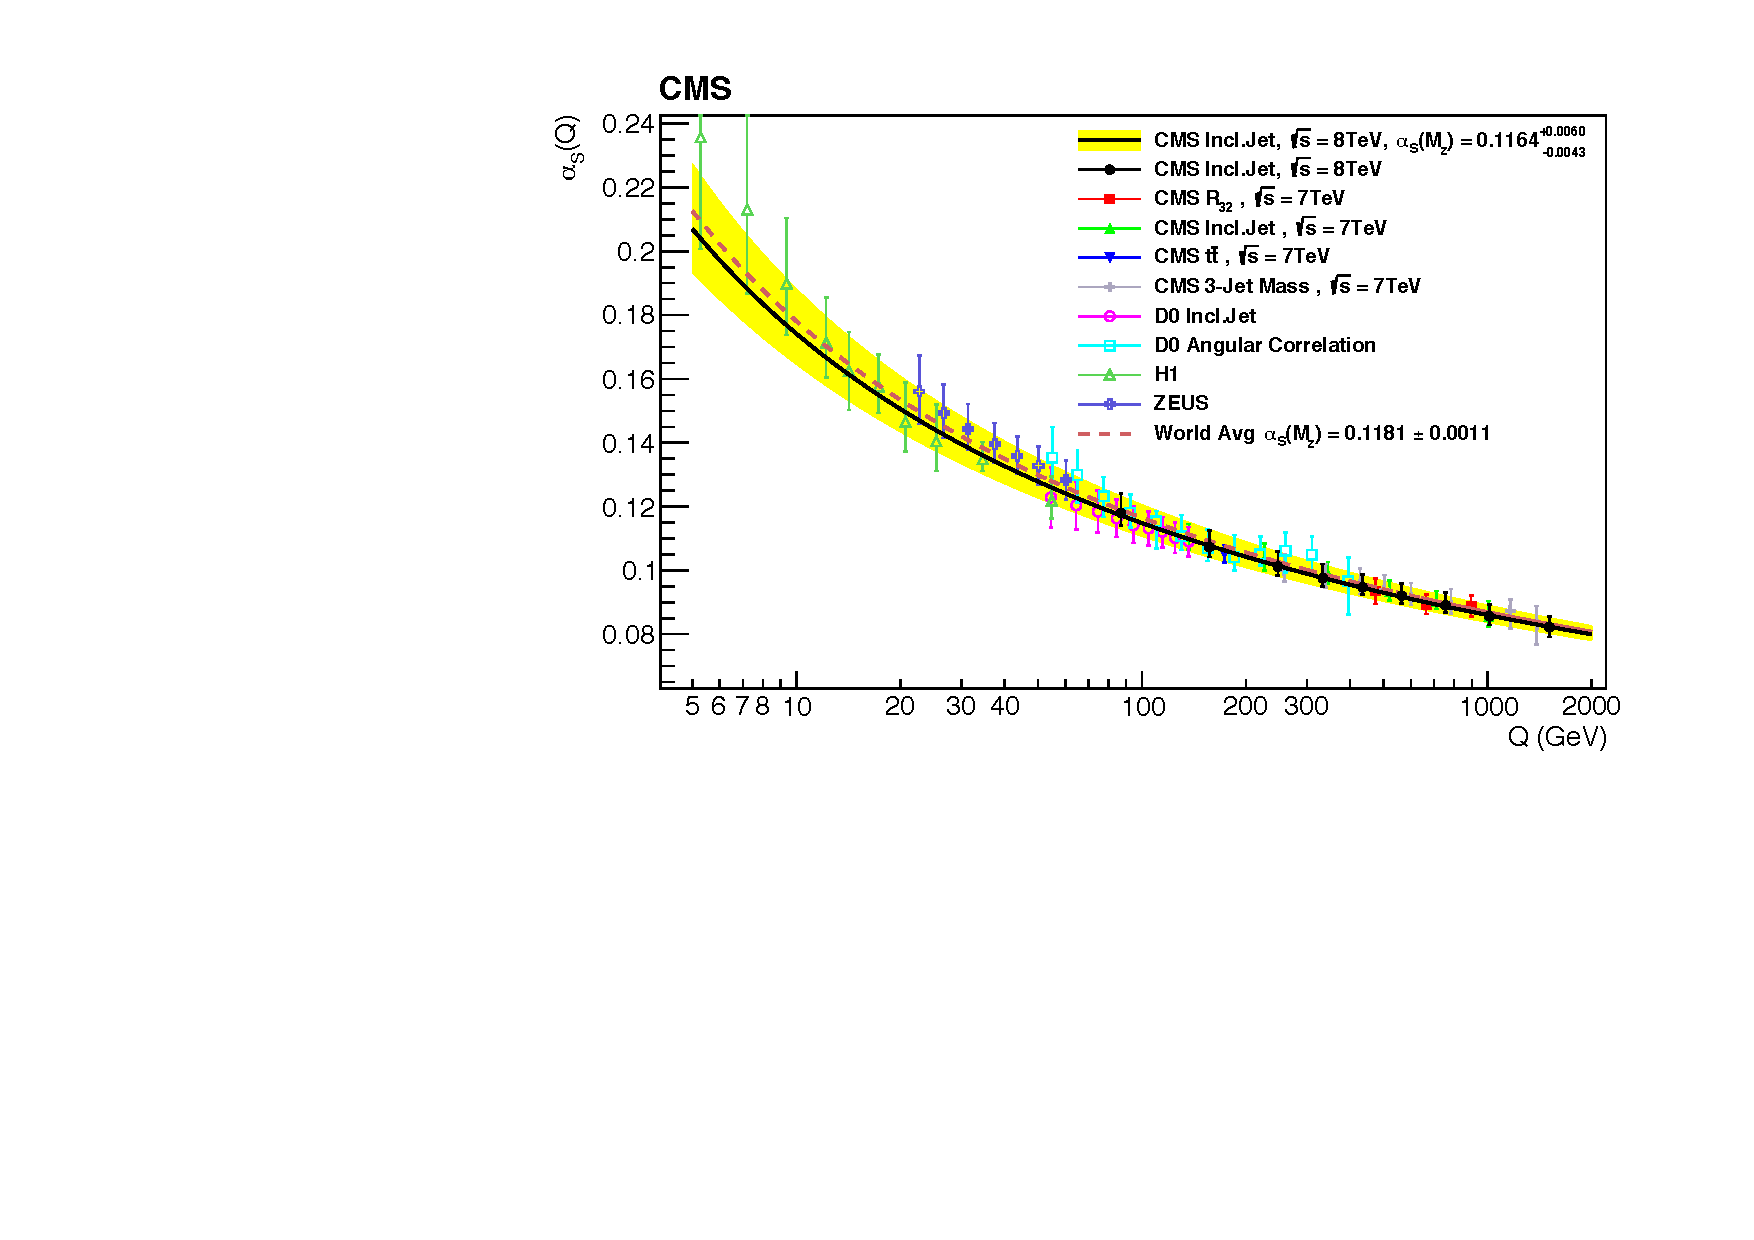
\includegraphics[width=0.7\textwidth]{Figures/standard_model/running}
    \caption{The running of the strong coupling constant $\alpha_s = \sfrac{g_s^2}{4\pi}$ as a function of the energy scale $Q$ as measured by experiments at the LHC, Tevatron, and HERA~\cite{CMSRunning}.}
    \label{fig:asymptotic_freedom}
\end{figure}

An observed effect of QCD is \textit{colour confinement} where quarks and gluons are never observed in isolation, but are always bound together in colour-neutral ($\text{SU}(3)$ invariant) states called hadrons.
This is illustrated by the qualitative picture in \Cref{fig:confinement}.
For an electromagnetic interaction, \Cref{fig:confinement_b}, the field is diluted over space.
However, for a strong interaction, \Cref{fig:confinement_c}, the exchanged gluons themselves interact, \Cref{fig:confinement_a}, effectively squeezing the colour field between the quarks into a \textit{colour flux tube} or a \textit{colour string}.
These strings have a constant energy density so two free quarks on opposite sides of the universe would theoretically result in a string of near-infinite energy.
As the theory is non-perturbative, there is no analytical description for confinement.
A consequence of confinement is hadronisation, the process by which high energy coloured particles form particle jets, which is described in \Cref{sec:jets}.

\begin{figure}[h]
    \centering
    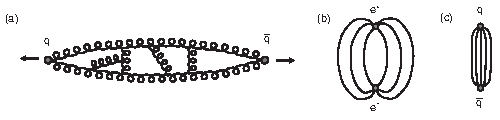
\includegraphics[width=0.8\textwidth]{Figures/standard_model/confinement.pdf}
    \begin{subfigure}{0pt}\phantomcaption{}\label{fig:confinement_a}\end{subfigure}
    \begin{subfigure}{0pt}\phantomcaption{}\label{fig:confinement_b}\end{subfigure}
    \begin{subfigure}{0pt}\phantomcaption{}\label{fig:confinement_c}\end{subfigure}
    \caption{Qualitative picture of the formation of colour strings due to interaction between the exchanged gluons from two quarks \cite{ModernParticlePhysics}.}.
    \label{fig:confinement}
\end{figure}

\subsection{\texorpdfstring{$\text{SU}(2)_L \times \text{U}(1)_Y \rightarrow$}{SU(2)xSU(1)-} Electroweak Theory}
\label{sec:electroweak}

In 1934 Fermi's description of $\beta$ decay~\cite{Fermi1934} hypothesized the existence of the weak nuclear force and allowed for the creation and annihilation of particles.
Around three decades later the Glashow-Weinberg-Salam model (GSW)~\cite{Glashow1961, Weinberg1967,Salam1964} was developed to unify the electromagnetic and weak forces using the combined $\text{SU}(2)_L \times \text{U}(1)_Y$.
As with all gauge theories, this introduces four gauge fields corresponding to each generator of the group.
\begin{align}
    \text{SU}(2)_L & \rightarrow W_\mu^a(a = 1, 2, 3) \\
    \text{U}(1)_Y  & \rightarrow B_\mu
\end{align}
The $\text{SU}(2)_L$ group is non-Abelian making this a Yang-Mills theory, and the structure constants are given by $f^{abc} = \epsilon^{abc}$, where $\epsilon^{abc}$ is the Levi-Civita symbol.
The generators of the group are the based on the three Pauli spin matrices $\sigma^i$.
\begin{equation}
    \label{eq:su2_generators}
    T^a \equiv I^a = \frac{\sigma^a}{2} \\
\end{equation}
\begin{equation}
    \sigma^1 = \begin{pmatrix} 0 & 1 \\ 1 & 0 \end{pmatrix},
    \quad \sigma^2 = \begin{pmatrix} 0 & -i \\ i & 0 \end{pmatrix},
    \quad \sigma^3 = \begin{pmatrix} 1 & 0 \\ 0 & -1 \end{pmatrix}.
    \label{eq:pauli_matrices}
\end{equation}
The strength tensors are given by
\begin{align}
    \label{eq:ew_field_strength_tensors}
    W_{\mu\nu}^a & = \partial_\mu W_\nu^a - \partial_\nu W_\mu^a - g \epsilon^{abc} W_\mu^b W_\nu^c, \\
    B_{\mu\nu}   & = \partial_\mu B_\nu - \partial_\nu B_\mu.
\end{align}
It is useful to split the fermion fields into left- and right-handed components using the chiral projection operators $P_{L/R} = \sfrac{1}{2} (1 \mp \gamma^5)$, where $\gamma^5 = i \gamma^0 \gamma^1 \gamma^2 \gamma^3$.
Experimentally the charged weak current has proved to maximally violate $\mathcal{P}$ symmetry.
This means that the interaction term must follow a V-A (vector-axial) coupling type which can be shown to be equivalent to a standard coupling to left-handed fermions only:
\begin{equation}
    \label{eq:v-a_coupling}
    \mathcal{L}_\text{V-A}
    = \frac{1}{2} \bar \psi \gamma^\mu (1 - \gamma^5) \psi W_\mu
    = \bar \psi \gamma^\mu P_L \psi W_\mu
    = \bar \psi P_R \gamma^\mu P_L \psi W_\mu
    = \bar \psi_L \gamma^\mu \psi_L W_\mu.
\end{equation}
Therefore, only left-handed fermions (and right-handed antifermions) carry non-zero weak isospin.
The covariant derivative is given by,
\begin{equation}
    \label{eq:ew_covariant_derivative}
    D_\mu = \partial_\mu - i g_W \frac{\sigma_a}{2} W_\mu^a - i g_Y \frac{Y}{2} B_\mu,
\end{equation}
where $g_W$ and $g_Y$ are the weak and hypercharge coupling constants respectively.
The Lagrangian for electroweak theory is,
\begin{align}
    \begin{split}
        \label{eq:ew_lagrangian}
        \mathcal{L}_\text{EW} = & - \bar{\psi}_L \left( \gamma^\mu g_W \frac{1}{2} \sigma^a W^a_\mu + \gamma^\mu g_Y \frac{Y}{2} B_\mu \right) \psi_L - \bar{\psi}_R \left( \gamma^\mu g_Y \frac{Y}{2} B_\mu \right) \psi_R \\
                                & - \frac{1}{4} W_{\mu\nu}^a W^{a,\mu\nu} - \frac{1}{4} B_{\mu\nu} B^{\mu\nu}.
    \end{split}
\end{align}
As a Yang-Mills theory, the gauge fields $W_\mu^a$ interact in quadratic and triple self-couplings.

The $2 \times 2$ Pauli matrices require two new components to the fermion wave function which are described as weak isospin doubles.
The left-handed fermions (and right-handed antifermions)
are placed in doublets which differ by a unit of charge.
Up-type quarks and neutrinos have a weak isospin of $\sfrac{1}{2}$, while down-type quarks and charged leptons have a weak isospin of $-\sfrac{1}{2}$.
The corresponding weak eigenstate doublets are given by,
\begin{equation}
    \label{eq:weak_isospin}
    \begin{pmatrix} \nu_e \\ e \end{pmatrix}_L,
    \begin{pmatrix} \nu_\mu \\ \mu \end{pmatrix}_L,
    \begin{pmatrix} \nu_\tau \\ \tau \end{pmatrix}_L,
    \begin{pmatrix} u \\ d' \end{pmatrix}_L,
    \begin{pmatrix} c \\ s' \end{pmatrix}_L,
    \begin{pmatrix} t \\ b' \end{pmatrix}_L.
\end{equation}
The right-handed fermions (and left-handed antifermions) do not carry isospin and are placed in singlets.
The effect of the charged weak interaction is therefore to rotate these doublets, effectively changing the flavour of the fermion\footnote{Since there is no other force through which the neutrinos can interact, there are no right-handed neutrinos in the SM.}.

The isospin doublets are described with respect to the weak eigenstates, which do not correspond to the observable mass eigenstates.
The down-type quarks by convention mix between the weak eigenstates ($d', s', b'$) and the mass eigenstates ($d, s, b$) through the CKM matrix~\cite{cabibbo1963},
\begin{equation}
    \label{eq:ckm_matrix}
    \begin{pmatrix} d' \\ s' \\ b' \end{pmatrix} =
    \begin{pmatrix} V_{ud} & V_{us} & V_{ub} \\ V_{cd} & V_{cs} & V_{cb} \\ V_{td} & V_{ts} & V_{tb} \end{pmatrix} \begin{pmatrix} d \\ s \\ b \end{pmatrix} =
    \begin{pmatrix} 0.974 & 0.224 & 0.004 \\ 0.221 & 0.975 & 0.041 \\ 0.009 & 0.042 & 1.014 \end{pmatrix} \begin{pmatrix} d \\ s \\ b \end{pmatrix},
\end{equation}
where the numerical values of the elements are determined experimentally~\cite{ParticleDataGroup}\footnote{The non-unitary nature of experimental values of the CKM matrix is in tension with the SM by 2.2$\sigma$}.
For the leptons, mixing is described with respect to the neutrinos and the PMNS matrix~\cite{PMNSMatrix}.
These matrices provide explanations for the observed neutrino oscillations and the CP violation of the weak sector.

\section{Electroweak Symmetry Breaking}
\label{sec:higgs}

GSW theory predicts 4 gauge fields $W^a_\mu$ and $B_\mu$ which do not correspond to the physical $W^\pm$, $Z$, and $\gamma$ bosons.
As a requirement of gauge invariance these fields are deemed to be massless, which is in contradiction to the observed massive $W^\pm$ and $Z$ bosons.
These discrepancies are resolved by the Brout-Englert-Higgs mechanism~\cite{Higgs1, Higgs2, Higgs3} (referred to hereafter as the Higgs mechanism), and the spontaneous symmetry breaking of the electroweak symmetry group (EWSB).
Spontaneous symmetry breaking is a phenomenon where the ground state of a system does not exhibit the same symmetries of the Lagrangian.
Experimental evidence for the electroweak theory first came in 1983 with the discovery of the W and Z bosons at CERN\@~\cite{WZ}.
Arguably the last major breakthrough in the field of particle physics was the discovery of the Higgs boson in 2012 by the ATLAS and CMS collaborations~\cite{ATLASHiggs, CMSHiggs}.

Consider a new scalar field given by a complex doublet,
\begin{equation}
    \phi = \begin{pmatrix} \phi^+ \\ \phi^0 \end{pmatrix} = \frac{1}{\sqrt{2}} \begin{pmatrix} \phi_1 + i \phi_2 \\ \phi_3 + i \phi_4 \end{pmatrix},
\end{equation}
embedded in a theory which observes the local $\text{SU}(2)_L \times \text{U}(1)_Y$ symmetry of the GSW model.
The Lagrangian density for the free scalar field, defined with the same covariant derivatives of \Cref{eq:ew_covariant_derivative}, is given by,
\begin{equation}
    \label{eq:higgs_lagrangian}
    \mathcal{L} = (D_\mu \phi)^\dagger (D^\mu \phi) - V(\phi).
\end{equation}
Here, $V(\phi)$ is a potential term describing the field self-interactions.
The specific potential encountered in the Higgs mechanism is defined as,
\begin{equation}
    \label{eq:higgs_potential}
    V(\phi) = \mu^2 \phi^\dagger \phi + \lambda (\phi^\dagger \phi)^2,
\end{equation}
where $\mu^2$ and $\lambda$ are free parameters of the theory with some restrictions.
The value of $\lambda$ is required to be positive to ensure the potential is bounded from below, allowing a stable vacuum state (the state of lowest energy).
The value of $\mu^2$ is constrained to be negative to allow for spontaneous symmetry breaking.
The vacuum state is found by minimizing the Hamiltonian of a system which corresponds to,
\begin{equation}
    \frac{\partial V}{\partial \phi} = 0 \Longrightarrow  \phi^\dagger \phi = -\frac{\mu^2}{2\lambda} \equiv \frac{v^2}{2},
\end{equation}
where $v$ is the vacuum expectation value of the field.

\begin{figure}[h]
    \centering
    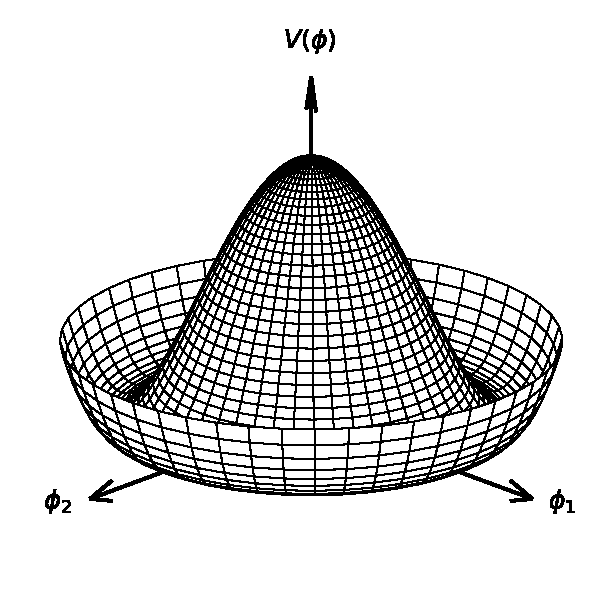
\includegraphics[width=0.5\textwidth]{Figures/standard_model/mexican_hat_potential}
    \caption{The form of the Higgs potential $V(\phi)$ if $\mu^2 < 0$ and $\lambda > 0$ respect to the first component of the complex doublet}
    \label{fig:mexican_hat}
\end{figure}

As shown in \Cref{fig:mexican_hat}, the potential has an infinite number of vacuum states satisfying this condition.
Physically the vacuum will fall into one of these states, spontaneously breaking the symmetry of the Lagrangian.
With no loss of generality, the physical vacuum state is chosen to be,
\begin{equation}
    \label{eq:higgs_vacuum}
    | 0 \rangle	= \frac{1}{\sqrt{2}} \begin{pmatrix} 0 \\ v \end{pmatrix}.
\end{equation}
In order to use perturbation theory the field $\phi$ is expanded about the vacuum state $|0\rangle$,
\begin{equation}
    \phi(x) = \frac{1}{\sqrt{2}} \begin{pmatrix} \phi_1(x) + i \phi_2(x) \\ v + \phi_3 + i \phi_4(x) \end{pmatrix}.
\end{equation}

The expected form of the symmetry breaking should result in the group of QED,
\begin{equation}
    \text{SU}(2)_L \times \text{U}(1)_Y \rightarrow_\text{EWSB} \text{U}(1)_\text{Q},
\end{equation}
where $Q$ refers to the electric charge.
The Goldstone theorem states that for every spontaneously broken continuous symmetry there exists a massless scalar boson; one for each generator of the group.
In EWSB, the broken symmetry should result in three massless Goldstone bosons, however there is no experimental evidence for such massless scalar particles.
The Higgs mechanism resolves this by absorbing the Goldstone bosons through an appropriate selection of gauge.
It's crucial to note that physical predictions remain unchanged regardless of the gauge, but by selecting the \textit{unitary gauge}, the Goldstone bosons vanish, and the fields in the Lagrangian represent the actual physical particles.
In the unitary gauge the scalar field is given by,
\begin{equation}
    \label{eq:higgs_unitary_gauge}
    \phi(x) = \frac{1}{\sqrt{2}} \begin{pmatrix} 0 \\ v + h(x) \end{pmatrix},
\end{equation}
where $h(x)$ is the physical massive Higgs field, the excitation of which is the Higgs boson $H$.

The relationship between weak isospin, hypercharge, and electric charge is given by,
\begin{equation}
    \label{eq:hypercharge}
    Q = I^3 + \frac{Y}{2}.
\end{equation}
Because the only surviving massless boson is the photon, $\text{U}(1)_\text{Q}$ must remain a symmetry of the vacuum state.
This is achieved by setting the electric charge of the vacuum state to zero, or equivalently $Y=1$.
Using the definitions from \Cref{eq:pauli_matrices} and \Cref{eq:ew_covariant_derivative} the covariant derivative is given by,
\begin{equation}
    \label{eq:higgs_covariant_derivative}
    D_\mu = \frac{1}{2}
    \begin{pmatrix}
        2 \partial_\mu + i g_W W_\mu^3 + i g_Y B_\mu &
        i g_W (W_\mu^1 - i W_\mu^2)                    \\
        i g_W (W_\mu^1 + i W_\mu^2)                  &
        2 \partial_\mu - i g_W W_\mu^3 + i g_Y B_\mu.
    \end{pmatrix}
\end{equation}
Combining this with the unitary gauge scalar field yields the first term of the Higgs Lagrangian,
\begin{align}
    \label{eq:higgs_lagrangian_1}
    \begin{split}
        (D_\mu \phi)^\dagger (D^\mu \phi) =
        \frac{1}{2} \partial_\mu h \partial^\mu h
        + \frac{1}{8} g_W^2 (W_\mu^1 + i W_\mu^2)(W^{1\mu} - i W^{2\mu})(v + h)^2
        \\
        + \frac{1}{8} (g_W W_\mu^3 - g_Y B_\mu)(g_W W^{3\mu} - g_Y B^\mu)(v + h)^2.
    \end{split}
\end{align}
One can identify the massive physical fields by the terms in \Cref{eq:higgs_lagrangian_1} that are quadratic in the gauge boson fields and do not contain the Higgs field.
\begin{equation}
    W^\pm_\mu = \frac{W^1_\mu \mp i W^2_\mu}{\sqrt{2}}
    \qquad
    Z_\mu = \frac{g_W W^3_\mu - g_Y B_\mu}{\sqrt{g_W^2 + g_Y^2}}
    \qquad
    A_\mu = \frac{g_W B_\mu + g_Y W^3_\mu}{\sqrt{g_W^2 + g_Y^2}}.
\end{equation}
Rewriting out \Cref{eq:higgs_lagrangian} in terms of the physical fields and in the unitary gauge gives,
\begin{equation}
    \label{eq:higgs_lagrangian_full}
    \resizebox{.99\hsize}{!}{$
            \begin{aligned}
                \mathcal{L}_{EW+H}
                 & = \underbrace{\vphantom{\frac{}{}} - \lambda v^2 h^2}_{H \text{ mass}}
                \underbrace{+\frac{1}{4} g_W^2 v^2 W^-_\mu W^{+\mu}}_{W \text{ mass}}
                \underbrace{+\frac{1}{8} g_Y^2 v^2 Z_\mu Z^\mu}_{Z \text{ mass}}                                                                                 \\
                 & \underbrace{+\frac{1}{2} g_W^2 v h W^-_\mu W^{+\mu}}_{HWW}
                \underbrace{+\frac{1}{4} g_W^2 h^2 W^-_\mu W^{+\mu}}_{HHWW}
                \underbrace{+\frac{1}{4} g_Y^2 v h Z_\mu Z^\mu}_{HZZ}
                \underbrace{+\frac{1}{8} g_Y^2 h^2 Z_\mu Z^\mu}_{HHZZ}                                                                                           \\
                 & \underbrace{+\frac{1}{2}(\partial_{\mu} h)(\partial^{\mu} h) - \lambda v h^3 + \frac{1}{4}\lambda h^4}_{h\text{ dynamics and self-couplings}}
                \underbrace{+\frac{1}{4} W^a_{\mu\nu} W^{a,\mu\nu} + \frac{1}{4} B_{\mu\nu} B^{\mu\nu}}_{\text{EW dynamics and self-couplings}}.
            \end{aligned}
        $}
\end{equation}
From the top row of \Cref{eq:higgs_lagrangian_full} the masses of each of the bosons can be identified,
\begin{equation}
    \label{eq:ew_masses}
    m_W = \frac{1}{2} g_W v
    \qquad
    m_Z = \frac{1}{2} v \sqrt{g_W^2 + g_Y^2}
    \qquad
    m_A = 0
    \quad
    m_H = \sqrt{2 \lambda} v.
\end{equation}
For convenience, the bottom row of \Cref{eq:higgs_lagrangian_full} includes the dynamics and self-couplings of the electroweak fields in their original form before EWSB.
Expanding this term with respect to the physical fields results in trilinear interactions between the photon and the $W^\pm$ bosons.
The free parameters of the GSW + Higgs mechanism are the electroweak coupling constants $g_W$ and $g_Y$, the Higgs self-coupling $\lambda$, and the vacuum expectation value $v$, all of which are determined experimentally.

The final piece of the SM is the generation of fermion masses through the Higgs mechanism.
Due to the different transformation properties of the left- and right-handed fermions, the standard mass term $m \bar \psi \psi$ mixes the left- and right-handed components and thus is not invariant under the electroweak symmetry group.
The Yukawa interaction term is introduced to couple each of the fermions doublets to the Higgs field.
For example the electron mass term is given by,
\begin{equation}
    \label{eq:yukawa}
    \begin{split}
        \mathcal{L}_\text{Yukawa} & = -g_e( \bar \psi_L \phi \psi_R + \bar \psi_R \phi^\dagger \psi_L)    \\
                                  & = -g_e \left[
            \begin{pmatrix} \bar \nu_e & \bar e \end{pmatrix}_L \begin{pmatrix} 0 \\ \frac{v + h}{\sqrt{2}} \end{pmatrix} e_R
            + \bar e_R \begin{pmatrix} 0 & \frac{v + h}{\sqrt{2}} \end{pmatrix} \begin{pmatrix} \nu_e \\ e \end{pmatrix}_L
        \right]                                                                                           \\
                                  & = -\frac{g_e v}{\sqrt{2}} \bar e e - \frac{g_e}{\sqrt{2}} \bar e e h,
    \end{split}
\end{equation}
where $g_e$ is the electron Yukawa coupling constant.
A similar prescription can be applied to other leptons, the up-type, and down-type quarks to yield the relationship of the fermion masses $m_f$ to the Yukawa coupling constants $g_f$ and the Higgs vacuum expectation value,
\begin{equation}
    \label{eq:fermion_mass}
    m_f = \frac{g_f v}{\sqrt{2}}.
\end{equation}

\section{Particle Jets}
\label{sec:jets}

In particle physics, jets are collimated streams of particles moving together in a cone-like structure that were initiated by a high-energy quark or gluon.
A common feature in high-energy collisions, jets are emergent phenomena that arise due to the nature of QCD.
Simply put, if a high-energy quark or gluon is emitted from a collision, it quickly radiates gluons.
Each of these emissions can themselves radiate gluons or split into quark-antiquark pairs, starting the process anew.
This continues until the energy of the particles is low enough that they form stable colour-neutral bound states.
Jets are therefore formed during the transition from the perturbative to the non-perturbative regimes of QCD.

Jet formation can be highlighted by the Feynman diagram in \Cref{fig:quark_gluon}.
Here a quark propagator, produced in some inelastic collision, radiates a gluon.
This matrix element becomes dominant when the virtual propagator is close to being on-shell.
This condition is satisfied by two limits which are essential in jet physics.
One is referred to as the \textit{collinear limit} where the angle between the quark and the gluon approaches zero.
This indicates preference for collinear radiation and explains why jets are collimated in the direction of the initiating particle\footnote{Jets are also collimated when measured in the lab frame due to the large boost of the initiating particle.}.
The other is the \textit{soft limit} where the energy of the gluon approaches zero.
Practically, this means that each time a parton is emitted, it is accompanied by a soft haze of radiation.
These conditions exist for all gauge theories, but are particularly important for QCD due the strength of $\alpha_s$ even at high energies.

\begin{figure}[h]
    \centering
    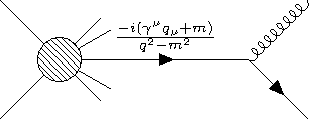
\includegraphics[width=0.5\textwidth]{Feynman/quark_gluon.pdf}
    \caption{Simple diagram of a quark emitted from a collision radiating a gluon. The matrix element of this process has a singularity when the virtual propagator is close to being on-shell ($q^2\approx m^2$) which is satisfied in the collinear and soft limits.}
    \label{fig:quark_gluon}
\end{figure}

Another view of jet formation is through the process of breaking colour strings between quarks.
From confinement, if two quarks were produced back-to-back in a collision, the colour field between them would be squeezed into a colour string with constant energy density.
As they move apart it becomes energetically favourable to create a quark-antiquark pair from the vacuum, leading to two new strings.
If the quarks are produced with enough energy, this process repeats until the energy is low enough that the stable colour-neutral bound states emerge as shown by \Cref{fig:hadronisation}.
Where exactly the strings break is ambiguous, resulting in the highly stochastic nature of jets.
The lightest hadrons are the most accessible to this process, which is why typically jets are composed primarily of pions ($\approx80\%$) and kaons ($\approx15\%$).

\begin{figure}[h]
    \centering
    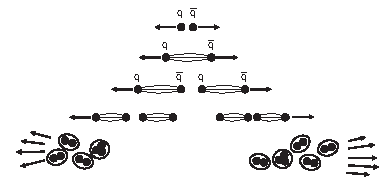
\includegraphics[width=0.8\textwidth]{Figures/standard_model/hadronisation.pdf}
    \caption{Qualitative picture of the formation of two jets via the splitting of colour flux-tubes causing hadronisation \cite{ModernParticlePhysics}.}
    \label{fig:hadronisation}
\end{figure}

While jets are essentially sets or clusters of many particles, they can also be defined by their own kinematics, calculated by summing up the four-momenta of all of their constituents.
Furthermore, even if the original parton was massless, the jet as a whole may have non-zero invariant mass due to noncollinear radiation.
The nature and shape of this radiation is characteristic of the properties of the initiating parton.
This point is crucial for understanding jet physics and defining jet reconstruction algorithms.

\section{Standard Model Limitations and Open Questions}
\label{sec:sm_limitations}

Predictions made by the SM have been confirmed to an extraordinary degree of precision in collider experiments, as shown by \Cref{fig:sm_precision}.
Despite this, there are several reasons to believe that the SM is not the final theory of particle physics.
Many perceived shortcomings of the SM lead to open questions, active areas of research, and proposed extensions to the theory.

For example, gravity is a notable omission from the SM owing to the lack of a renormalizable QFT for gravity.
Candidate theories for a quantum theory of gravity include string theory and loop quantum gravity~\cite{GravityQFT}.
However, gravity is so weak that it is unlikely a theory of quantized gravity could even make testable predictions at the energies accessible by current experiments.

\begin{figure}
    \centering
    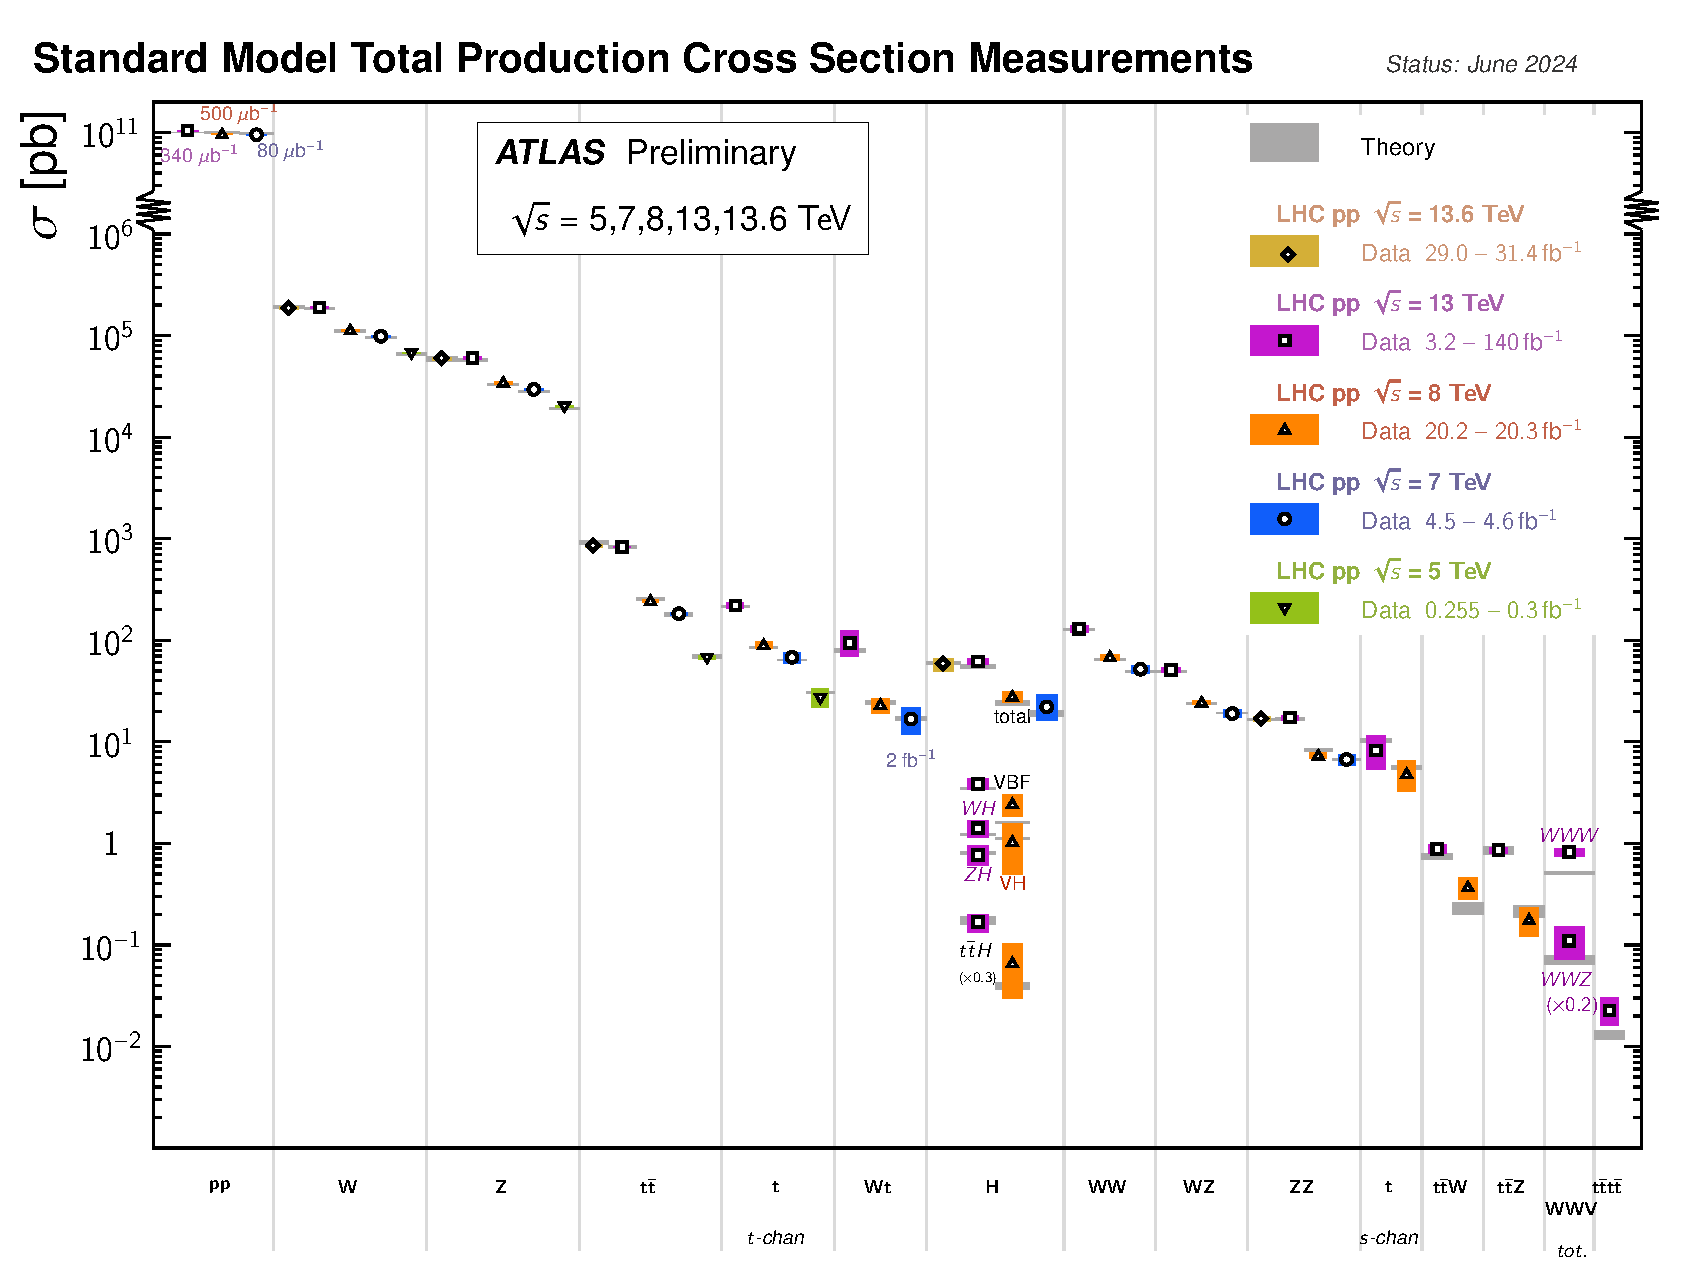
\includegraphics[width=0.7\textwidth]{Figures/standard_model/sm_summary.pdf}
    \caption{Comparison of the total production cross-sections of various processes predicted by the SM and measured by the ATLAS experiment \cite{ATLAS:2024cgh}.}
    \label{fig:sm_precision}
\end{figure}

Cosmological observations dating back to the 1930s~\cite{GalaxyRotation} have shown that the majority of the gravitational effects in the universe is not a result of visible matter.
This was first observed by the movements of galaxies within clusters~\cite{GalaxyRotation}, but has since been independently supported by measurements of the rotation of galaxies themselves~\cite{DistributionDarkMatter, EvidenceDarkMatter,NumericalStudyStability}, gravitational lensing~\cite{GravitationalLensMagnification, Lensing1, Lensing2},
hot gas in galaxy clusters~\cite{HotGas}, and the cosmic microwave background~\cite{Planck2018Results}.
The current theory to explain these phenomena is the presence of cold dark matter (CDM) which accounts for 85\% of the mass content in the universe~\cite{Planck2018Results}.
In this model, CDM particles must be stable, massive, and (at most) weakly interacting.
There is no candidate in the SM that fits this description.
Furthermore, in the $\Lambda$CDM model of cosmology the dominant energy in the universe is \textit{dark energy}~\cite{LCDM1, LCDM2, LCDM3, LCDM4}, a positive pressure of the vacuum causing the universe to expand at an accelerating rate for which the SM offers no explanation.

In the SM, anti-matter is treated as a mirror image of matter.
However, there is a significant discrepancy between the amount of matter and anti-matter in the universe~\cite{AlexDM1, AlexDM2}.
There exist two possibilities for this discrepancy; either the universe began with a preference for matter over anti-matter, or the universe was initially symmetric, and some process called \textit{baryogenesis}~\cite{BaryosynthesisOriginGalaxies}, occurred to create the imbalance.
While there is no clear evidence for either scenario, the latter is more appealing to many physicists.
The Sakharov conditions~\cite{Sakharov1967} for baryogenesis are that it violates baryon number, C and CP symmetry, and must have occurred before the universe reached thermal equilibrium.
CP violation is present in the SM from the CKM and PMNS matrices, but it is not sufficient to explain the observed matter-antimatter asymmetry.
It is hoped that there exists new physical processes beyond the SM that induces the much larger CP violation required for baryogenesis.

The above issues are associated with the SM's inability to describe cosmological phenomena.
An additional set of ``issues'' are derived from aesthetic or philosophical considerations.
The SM has 19 free parameters that must be determined experimentally, a value considered by many to be too large to be considered a fundamental theory.
Another issue is the \textit{hierarchy problem}.
In a QFT, physical observables are determined by the sum of all possible Feynman diagrams, which often includes divergent terms.
These divergences are removed by renormalization which fixes the parameters of the theory to the observed values.
However, in the case of the Higgs mass, the one-loop corrections are around 16 orders of magnitude larger than the observed value.
To resolve this the bare mass of the Higgs must be fine-tuned to an accuracy of 1 part in $10^{16}$, which many physicists find unsatisfactory.
Finally, the unification of QED and the weak force led many physicists to develop Grand Unified Theories (GUTs)~\cite{GUT1, GUT2} which predict that all forces in the SM are unified at high energies.
Many of the predictions of GUTs, such as proton decay, have not been observed, and the energy scale at which the forces unify is far beyond the reach of current experiments.

% 
\chapter{The Large Hadron Collider and the ATLAS Detector}
\label{ch:lhc_atlas_detector}

The Large Hadron Collider (LHC)~\cite{LHCMachine,LHC1,LHC2, LHC3} is a synchrotron collider located at the Conseil Européen pour la Recherche Nucléaire (CERN) near Geneva, Switzerland.
It is also the world's most powerful particle accelerator, providing both proton-proton ($pp$) and heavy ion collisions at the high energy frontier.
At maximum speed, the protons in the LHC are only $3~\mps$ slower than the speed of light.

Four primary experiments utilize the $\TeV$ scale collisions generated at each of the four interaction points (IPs) of the LHC.
Two general-purpose experiments, ATLAS~\cite{ATLAS} and CMS~\cite{CMS}, employ hermetic detectors to study various physics processes.
The LHCb experiment~\cite{LHCb} focuses on measuring the properties of B mesons and other particles containing b-quarks, which are significant for understanding CP violation.
The Alice experiment~\cite{ALICE} investigates the properties of quark-gluon plasma, a state of matter believed to have existed in the early universe.
Additionally, the LHC hosts several smaller, highly specialized experiments including LHCf~\cite{LHCf}, TOTEM~\cite{TOTEM}, MoEDAL~\cite{MoEDAL}, FASER~\cite{FASER}, and SND@LHC~\cite{SNDLHC}.
All LHC experiments strive to answer fundamental questions about the universe; to test the predictions of the Standard Model of particle physics or to search for new physics beyond it.

This section describes common collider physics definitions, such as the coordinate system and luminosity,
the LHC along with its injector chain, and the ATLAS experiment.
As the focus of this work is on data and tools for $pp$ collisions at the LHC, the discussion is limited to this context.
Additionally, the components of this thesis which utilized official ATLAS simulation and software, \Cref{ch:spice}, were limited to tracks and jets.
Therefore, the information provided here is focused on these topics only.

\section{The Large Hadron Collider}

The LHC is a somewhat circular collider with a circumference of $26.7~\km$.
It is closer to an irregular octagon with rounded corners and approximately $ 530~\m $ long straight sections, housed within a tunnel whose depth varies between $45~\m$ and $170~\m$ underground.

The machine consists of two ring acceleration pipes, each carrying a separate beam of protons or heavy ions that are accelerated in opposite directions.
The beams are surrounded by 1232 superconducting niobium-titanium (NbTi) dipole magnets that generate an $8.33~\tesla$ magnetic field to bend the protons around the curved sections of the ring.
Many more higher-order multipole magnets are used for beam insertion, cleaning, dumping, and focusing towards the experiment IPs.
Along one of the straight sections, 16 superconducting radiofrequency cavities, eight per beam, operate at $400~\MHz$ to accelerate the protons to their maximum energy.
The LHC was designed to deliver a centre-of-mass energy of $\sqrt{s}=14~\TeV$ but has yet to reach this due to technical limitations.

The beams are not continuous streams of protons but are instead segmented into bunches, each containing on the order of $10^{11}$ particles.
The radiofrequency cavities are tuned to ensure that these bunches are tightly packed, each as long as $7.5~\cm$ and separated by only $25~\ns$.
For collisions to occur, the bunches from the two opposing beams are compressed to a space of $64~\um$, around the width of a strand of hair, and made to pass through each other.
Even with such compression and more than a hundred billion protons in each bunch, the average number of interactions per bunch crossing \avemu is less than 100.

\subsection{The CERN Accelerator Complex}

The LHC is a synchrotron, meaning that it cannot accelerate particles from rest.
Therefore, it is only the final stage of the CERN accelerator complex, which is shown in \Cref{fig:cern_accelerator_complex}.
Each stage in the chain of accelerators increases the energy of the particles within before passing them to the next stage.
Before 2020, the chain began with the Linear Accelerator (Linac) 2, which accelerated protons to $50~\MeV$.
The input to Linac2 was hydrogen gas, stripped of its electrons by a strong electric field.
Following Run 2, the chain was updated to begin with Linac4, which operates on negative hydrogen ions, not protons.
This change reduces the beam loss, allowing more particles to accumulate in the next stage.
Furthermore, Linac4 introduce a three-fold increase in beam energy, outputting particles at $160~\MeV$.
The Linacs feed the Proton Synchrotron Booster (PSB), which increases the energy to $2~\GeV$ and also serves to strip the electrons from the hydrogen ions.
From the PSB, the protons are passed to the Proton Synchrotron (PS), which accelerates them to $26~\GeV$, and then to the Super Proton Synchrotron (SPS), which accelerates them to $450~\GeV$.
From there, they are injected into the LHC.
This entire process takes a few seconds, but several minutes are required to fill the entire bunch train of the LHC.
The LHC then accelerates the bunches to the final energy, which, as of Run 3, is $6.8~\TeV$ per beam.

\begin{figure}
    \centering
    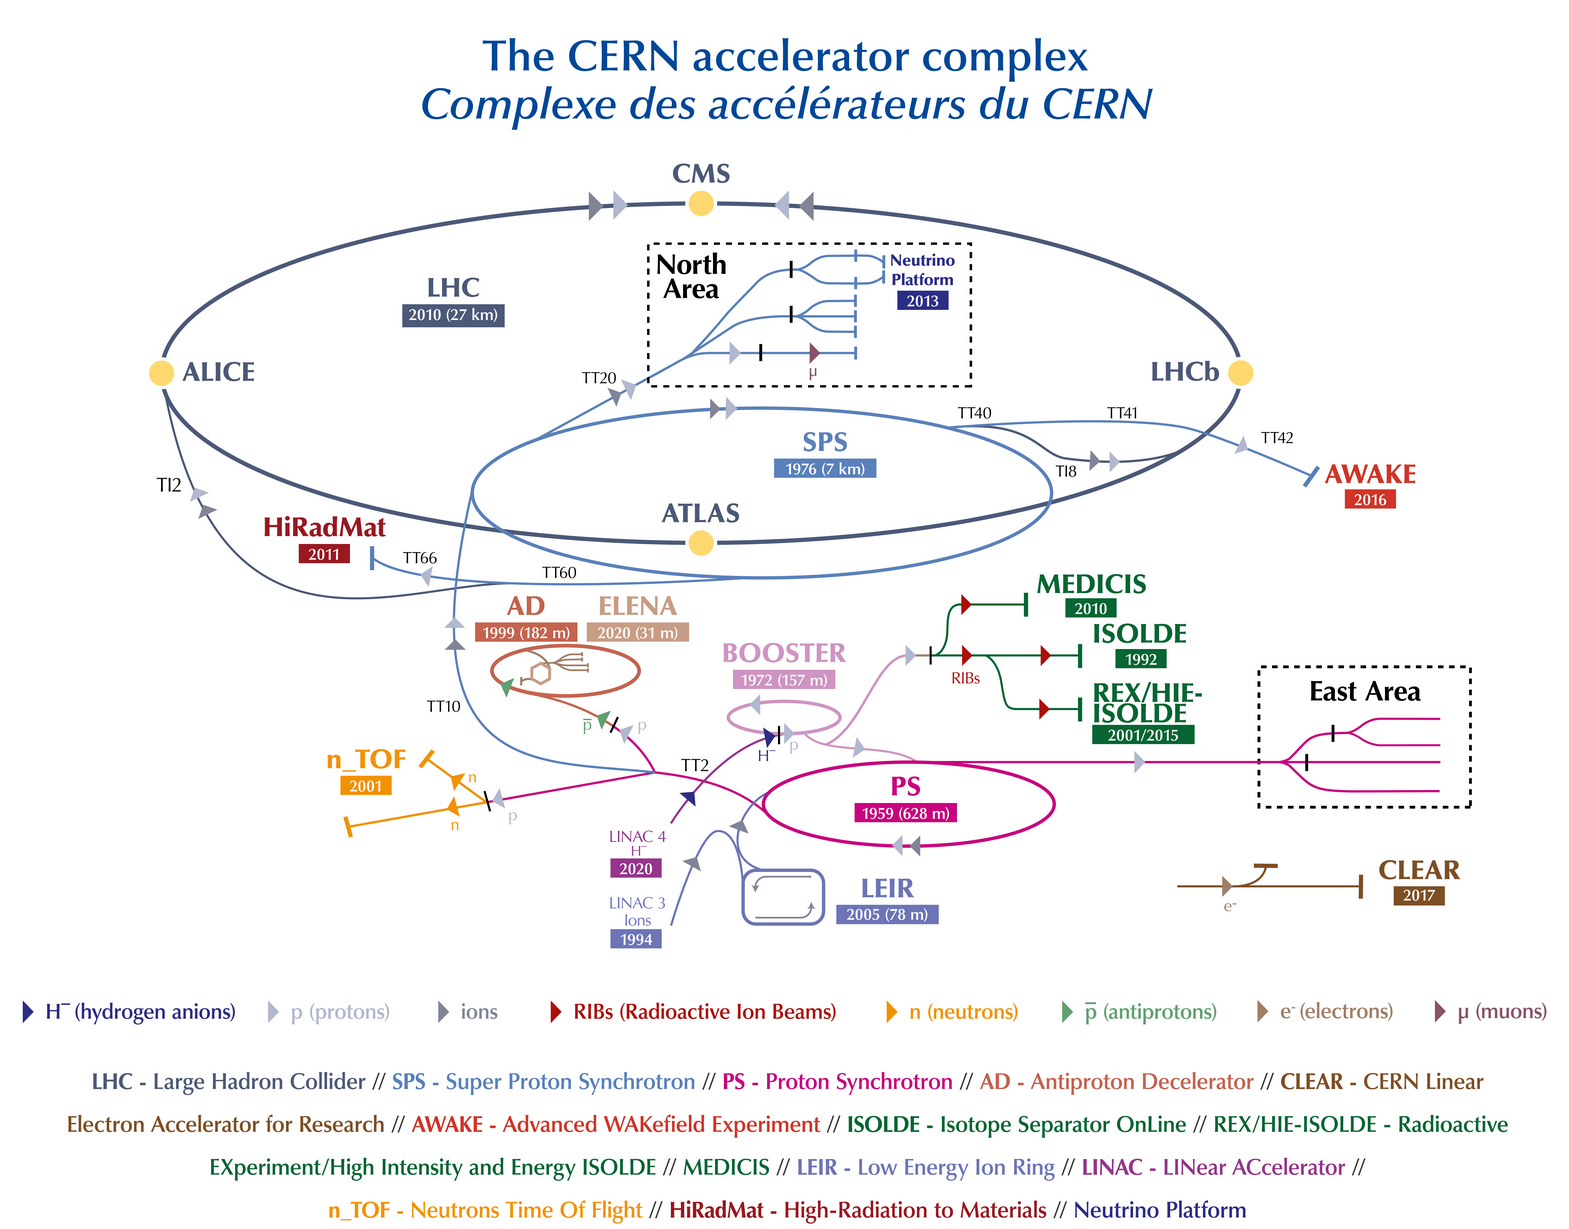
\includegraphics[width=0.99\textwidth]{Figures/cern_atlas/complex.png}
    \caption{The layout of the CERN accelerator complex as of 2022~\cite{CERNAC}.}
    \label{fig:cern_accelerator_complex}
\end{figure}

\subsection{Coordinate Systems}

In collider experiments, the typical coordinate system places the origin at the nominal IP, which, for hermetic detectors like ATLAS, Alice, and CMS, is at the centre of the detector.
The coordinate systems used by these experiments are right-handed, as shown in \Cref{fig:atlas_coordinate_system}, with the $z$-axis points along the beamline, the $y$-axis pointing upwards, and the $x$-axis pointing towards the centre of the LHC ring.
The transverse plane is defined as the plane perpendicular to the beam axis and is spanned by the $x$ and $y$ coordinates.

A polar representation is also often used, where the azimuthal angle $\phi$ is measured in the transverse plane from the $x$-axis, and the polar angle $\theta$ is measured from the $z$-axis.
The polar angle is frequently replaced with pseudorapidity $\eta$, defined as
\begin{equation}
    \eta = -\ln \left( \tan \left( \frac{\theta}{2} \right) \right).
\end{equation}
Differences in pseudorapidity are Lorentz invariant under boosts in the direction of the beamline, making it a useful quantity for describing the products of high-energy collisions.

Angular distances between objects are often measured in $\Delta R = \sqrt{(\Delta \eta)^2 + (\Delta \phi)^2}$, where $\Delta \eta$ and $\Delta \phi$ are the differences in pseudorapidity and azimuthal angle.
For collision products, a key observable is a transverse momentum $\pt=\sqrt{p_x^2 + p_y^2}$, where $p_x$ and $p_y$ are the components of the momentum in the transverse plane.

\begin{figure}
    \centering
    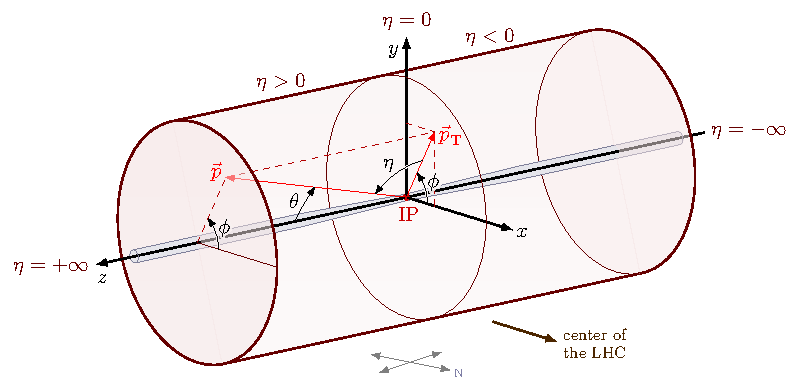
\includegraphics[width=0.6\textwidth]{Feynman/coordinate.pdf}
    \caption{The right-handed coordinate system used by the ATLAS experiment.}
    \label{fig:atlas_coordinate_system}
\end{figure}

\subsection{Cross-Section and Luminosity}

The cross-section, denoted by $\sigma$, indicates the likelihood of an interaction between two colliding particles.
Although calculating the cross-section involves quantum mechanical transition matrix elements and phase space integrals, it can be likened to the effective cross-sectional area of the particles participating in the interaction.

The total number of interactions $N$ depends on the cross-section of the process $\sigma$ and the integrated luminosity $L_{\text{int}}$ by the formula,
\begin{equation}
    N = \sigma L_{\text{int}} = \sigma \int \mathcal{L}(t) dt,
\end{equation}
where $\mathcal{L}(t)$ is the instantaneous luminosity.
This measures how tightly packed colliding particles are in a unit of space and time.
For two colliding beams with Gaussian densities, the instantaneous luminosity is given by
\begin{equation}
    \mathcal{L}(t) = \frac{N_1 N_2 f}{4 \pi \sigma_x \sigma_y} S(\theta_c),
\end{equation}
where $N_1$ and $N_2$ are the number of particles in each beam, $f$ is the frequency of bunch crossings, $\sigma_x$ and $\sigma_y$ are the root-mean-square beam widths in the $x$ and $y$ directions, and $S(\theta_c)$ is the geometric reduction factor due to the crossing angle $\theta_c$.
This last factor exists because the beams do not collide head-on, as this would result in multiple collision points, so they are crossed at a finite angle $\theta_c$.
This reduces the overlap of the beams when they pass through one another, reducing the effective luminosity.
For the $pp$ collisions at the LHC $S(\theta_c)$ is approximately $0.61$.
Even with this finite angle, long-range beam-beam interactions can still occur and must be accounted for.

The LHC was designed to deliver $\mathcal{L}(t) = 10^{34}~\unit{\centi\meter^{-2}\second^{-1}}$ at the IPs of ATLAS and CMS.
However, this has not been constant over the years, and each experiment independently measures the luminosity using well-understood processes.
The total integrated luminosity delivered by the LHC and recorded by ATLAS is shown in \Cref{fig:luminosity}.
The LHC's instantaneous luminosity has increased with each run and this is particularly beneficial for measurements on rare events where the uncertainty is statistically limited.

\begin{figure}
    \centering
    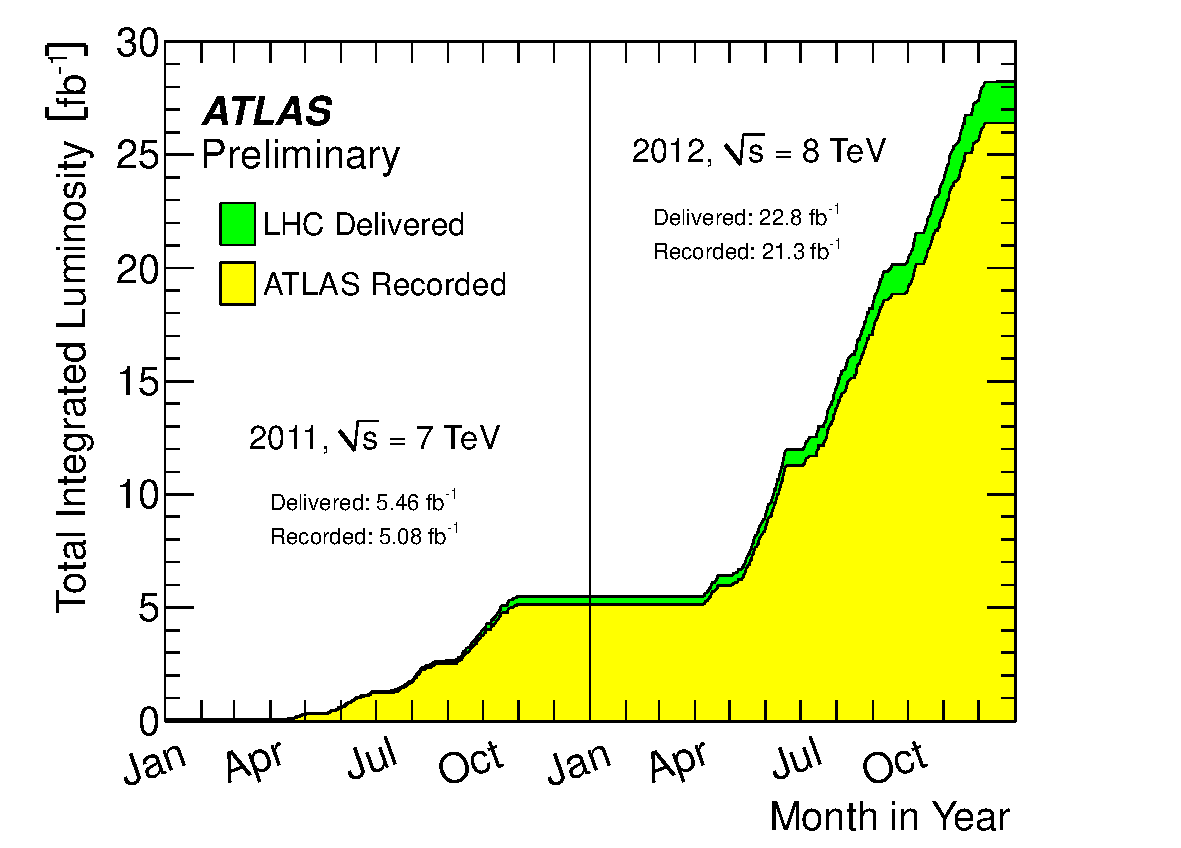
\includegraphics[width=0.32\textwidth]{Figures/cern_atlas/lumi1.pdf}
    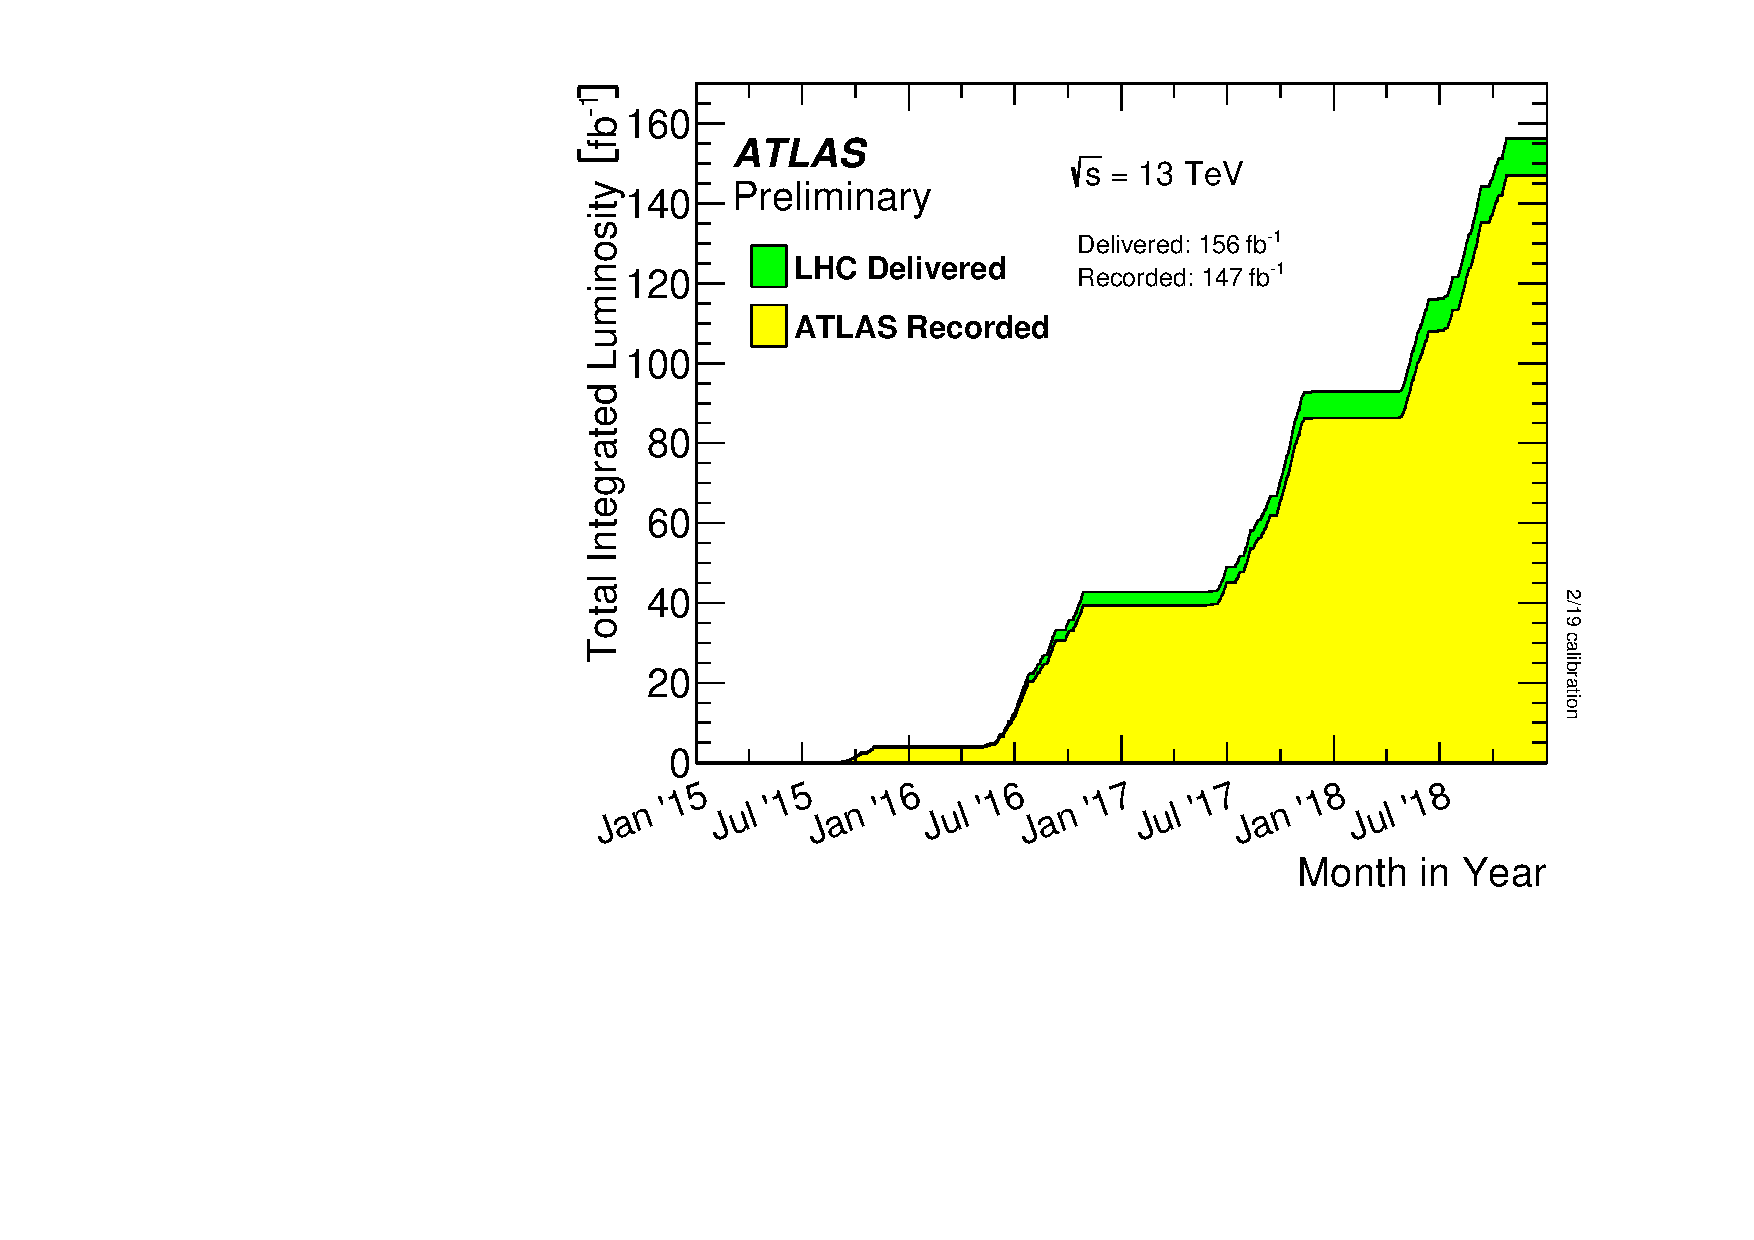
\includegraphics[width=0.32\textwidth]{Figures/cern_atlas/lumi2.pdf}
    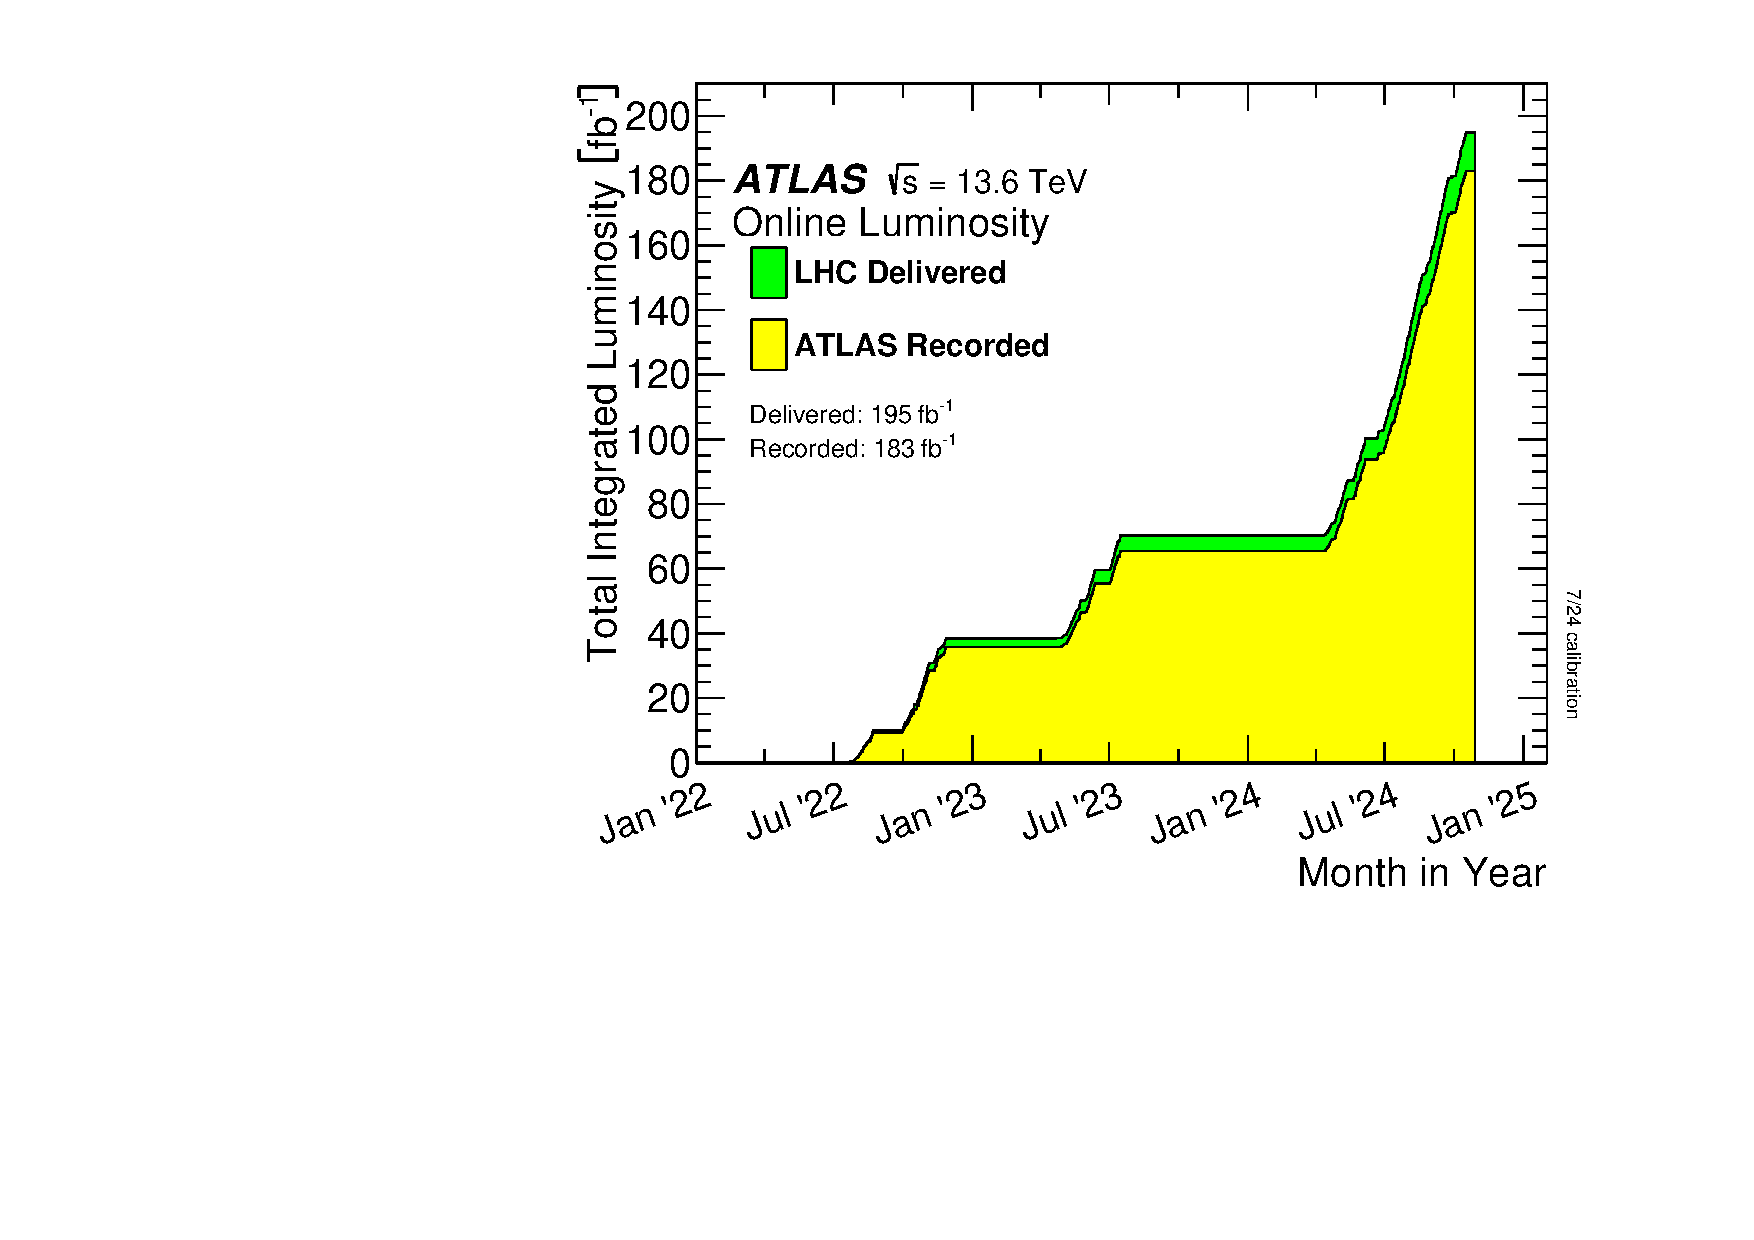
\includegraphics[width=0.32\textwidth]{Figures/cern_atlas/lumi3.pdf}
    \caption{The total integrated luminosity delivered by the LHC and recorded by the ATLAS experiment for Run 1 (left)~\cite{run1data}, Run 2 (middle)~\cite{run2data}, and Run 3 (right)~\cite{run3data}.}
    \label{fig:luminosity}
\end{figure}

\subsection{Pileup}

The increase in luminosity between Run 1 and Run 3 was in part achieved by raising the number of protons per bunch.
This in turn leads to more particle interactions per bunch crossing.
One of the undesirable effects of this is the large amount of overlapping signals in the detector which can degrade the resolution and efficiency of reconstruction algorithms.

Each bunch crossing in the collider generates a distinct event for analysis.
While the average number of interactions per crossing has increased with each LHC run, \Cref{fig:pileup} shows a wide distribution of interaction counts within each run.
Generally, only one of these interactions -- the hard scatter -- produces the high-energy particles captured by the detector and thus is of primary interest.
The remaining ``soft scatters'' are low-energy interactions that are known as in-time pileup.
Detector materials have a response and reset time, which can lead to residual signals from previous crossing being rerecorded, this is known as out-of-time pileup.
Filtering out signals from all pileup sources is crucial for accurate data analysis and poses a significant challenge as the LHC's luminosity increases.

\begin{figure}
    \centering
    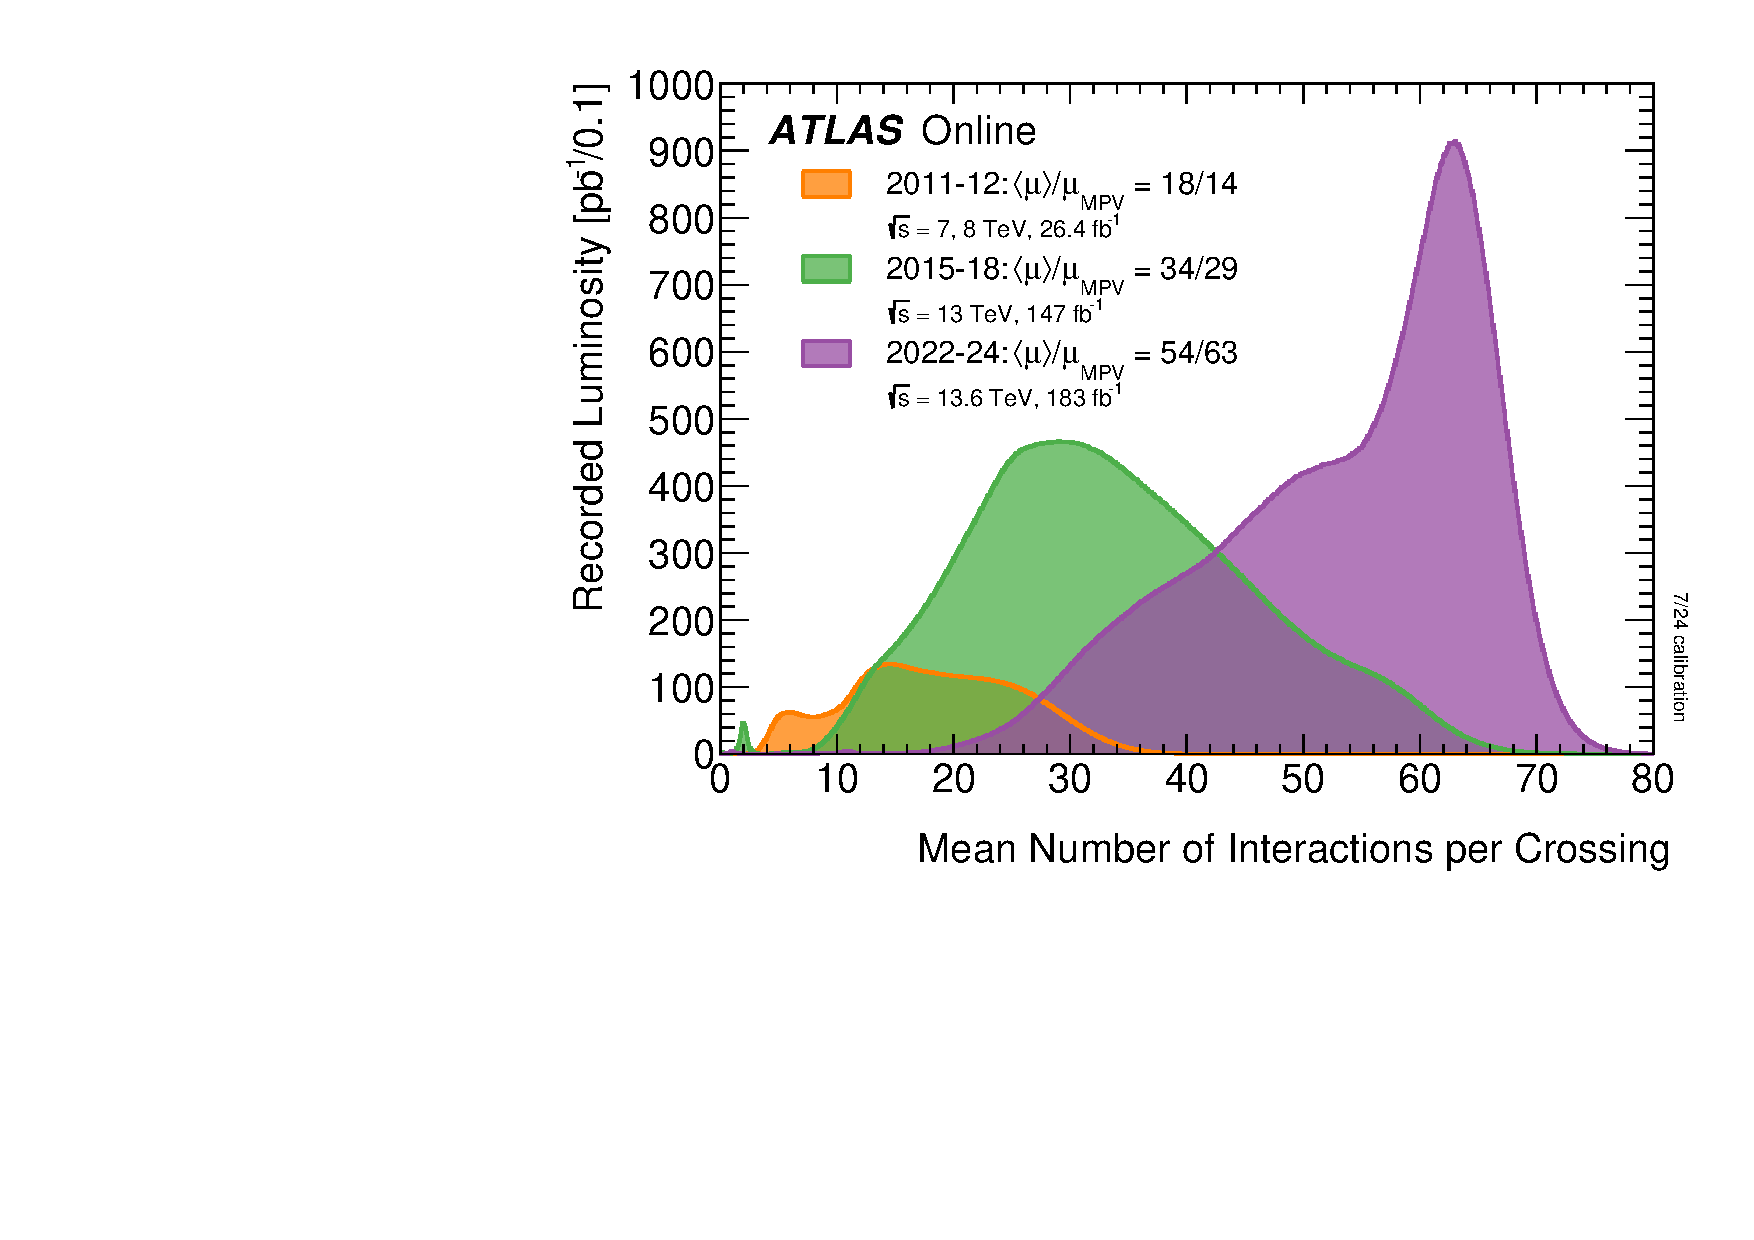
\includegraphics[width=0.6\textwidth]{Figures/cern_atlas/mu_run123.pdf}
    \caption{The distribution of the number of interactions per bunch crossing over the three LHC runs as measured by the ATLAS experiment~\cite{run3data}.}
    \label{fig:pileup}
\end{figure}

\subsection{LHC Runs}

The LHC operates on multi-year runs, the first beginning in 2010.
In between each run is a period of \textit{long-shutdown}, allowing for maintenance and upgrades to both the accelerator and the experiments.
The various run properties are shown in \Cref{tab:lhc_runs}.
Due to an electrical fault damaging many of the superconducting magnets in 2008, Run 1 was much delayed and operated at a reduced $\sqrt{s}=7~\TeV$ using a sparse bunch structure, only colliding at $20~\MHz$.
In 2012, the energy was increased to $\sqrt{s}=8~\TeV$.
The total delivered luminosity of the run was $28.4~\ifb$.
Run 2 spanned from 2015 to 2018, with an increased energy of $\sqrt{s}=13~\TeV$, a bunch crossing rate of $40~\MHz$, and a total integrated luminosity of $156~\ifb$.
Run 3 began in 2022 and is expected to continue until 2026 and has already surpassed Run 2 with $195~\ifb$ of data delivered~\cite{run3data}.

\begin{table}[h!]
    \centering
    \caption{Overview of the different LHC runs~\cite{LHCRun2,LHCRun3,run1data, run2data, run3data}. Values for Run 3 are preliminary as data is still being collected.}
    \label{tab:lhc_runs}
    \resizebox{\textwidth}{!}{
        \begin{tabular}{lcccccc}
            \toprule
                              & $\sqrt{s}~[\TeV]$ & $\mathcal{L}_\text{int}~[\ifb]$ & Protons per bunch     & Bunch spacing $[\ns]$ & \avemu \\
            \midrule
            Run 1 (2010-2011) & 7                 & 5.5                             & $1.45 \times 10^{11}$ & 50                    & 10     \\
            Run 1 (2012)      & 8                 & 22.8                            & $1.6 \times 10^{11}$  & 50                    & 21     \\
            Run 2 (2015-2028) & 13                & 156                             & $1.25 \times 10^{11}$ & 25                    & 34     \\
            Run 3 (2022-)     & 13.6              & 195                             & $1.8 \times 10^{11}$  & 25                    & 50     \\
            \bottomrule
        \end{tabular}
    }
\end{table}

\section{The ATLAS Experiment}

The ATLAS experiment~\cite{ATLAS, ATLASRun3} is one of the four primary experiments at the LHC\@.
It is the largest particle detector of the four, weighing $7000$ tonnes and measuring $44$ m long and $25$ m in diameter.
It is a general-purpose detector designed to explore a wide range of physics phenomena.
To achieve this, it has multiple sub-detectors designed to capture a broad range of outgoing products from the $pp$ collisions.
The ATLAS detector is shown in \Cref{fig:atlas_detector}.

The detector is hermetic, meaning it covers nearly the entire solid angle of $4\pi$.
It is arranged in concentric cylindrical-like layers around the IP\@.
Each layer contains a barrel region, which wraps around the beamline, and end-cap regions, which cover the flat edges of the cylinder on either side.

This section describes the ATLAS detector, focusing on the tracking systems.
These systems provide precise position and momentum measurements of charged particles, which are used to reconstruct particle trajectories and vertices.

\begin{figure}[htb]
    \centering
    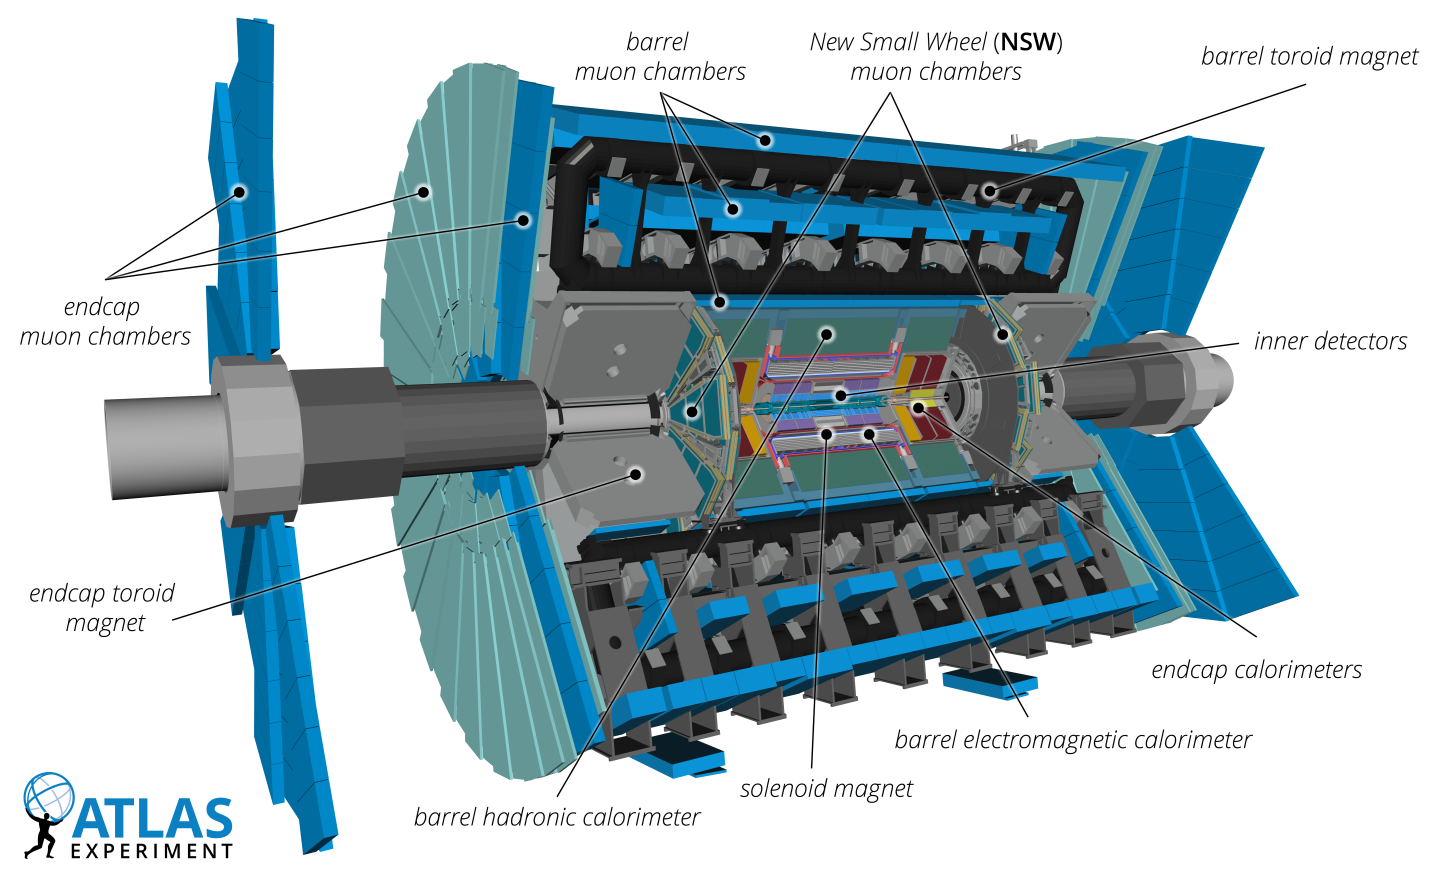
\includegraphics[width=0.99\textwidth]{Figures/cern_atlas/ATLAS.png}
    \caption{The ATLAS detector at the LHC\@. Image taken from Ref.~\cite{ATLASRun3}.}
    \label{fig:atlas_detector}
\end{figure}

\subsection{Inner Detector}

The Inner Detector (ID) is the innermost sub-detector of ATLAS and is shown in \Cref{fig:atlas_inner_detector}.
It comprises three sub-detectors: the Pixel Detector, the Semi-Conductor Tracker (SCT), and the Transition Radiation Tracker (TRT).
It is designed to capture charged particle signals with a pseudorapidity $|\eta| < 2.5$.
These signals are clustered into points in space where the particles have ionized the detector material.
These points can be used to reconstruct the charged particle's trajectory -- track -- as it propagates out from the centre of the detector.

The ID is immersed in a $2~\tesla$ axial magnetic field generated by a 5.8 m long superconducting solenoid magnet containing over $9\km$ of NbTi wire.
The magnetic field causes the particles to bend in a plane perpendicular to the beamline, tracing out a helical path whose curvature is proportional to $q/p$, where $q$ is the charge of the particle and $p$ is the magnitude of its momentum.

A fully reconstructed track is characterized by five parameters, which are shown in \Cref{fig:track_parameters}.
These include the charge-to-momentum ratio $q/p$, the azimuthal angle $\phi$, the polar angle $\theta$.
By tracing the track back to the beamline, the longitudinal $z_0$ and transverse $d_0$ impact parameters are determined at the point of closest approach to the IP\@.
These impact parameters represent the distances measured in each respective direction.
The relative $\pt$ resolution of the ID is described as,
\begin{equation}
    \sigma(\frac{1}{\pt}) = 0.36 \oplus \frac{13}{\pt \sin(\theta)}~\TeV
\end{equation}
where $\oplus$ denotes a sum in quadrature.

\begin{figure}[htb]
    \centering
    \includegraphics[width=0.6\textwidth]{Figures/cern_atlas/Track.png}
    \caption{The main parameters of a reconstructed track in the ATLAS Inner Detector. Image taken from Ref.~\cite{ATLASTrackingSoftware}.}
    \label{fig:track_parameters}
\end{figure}

\begin{figure}[htb]
    \centering
    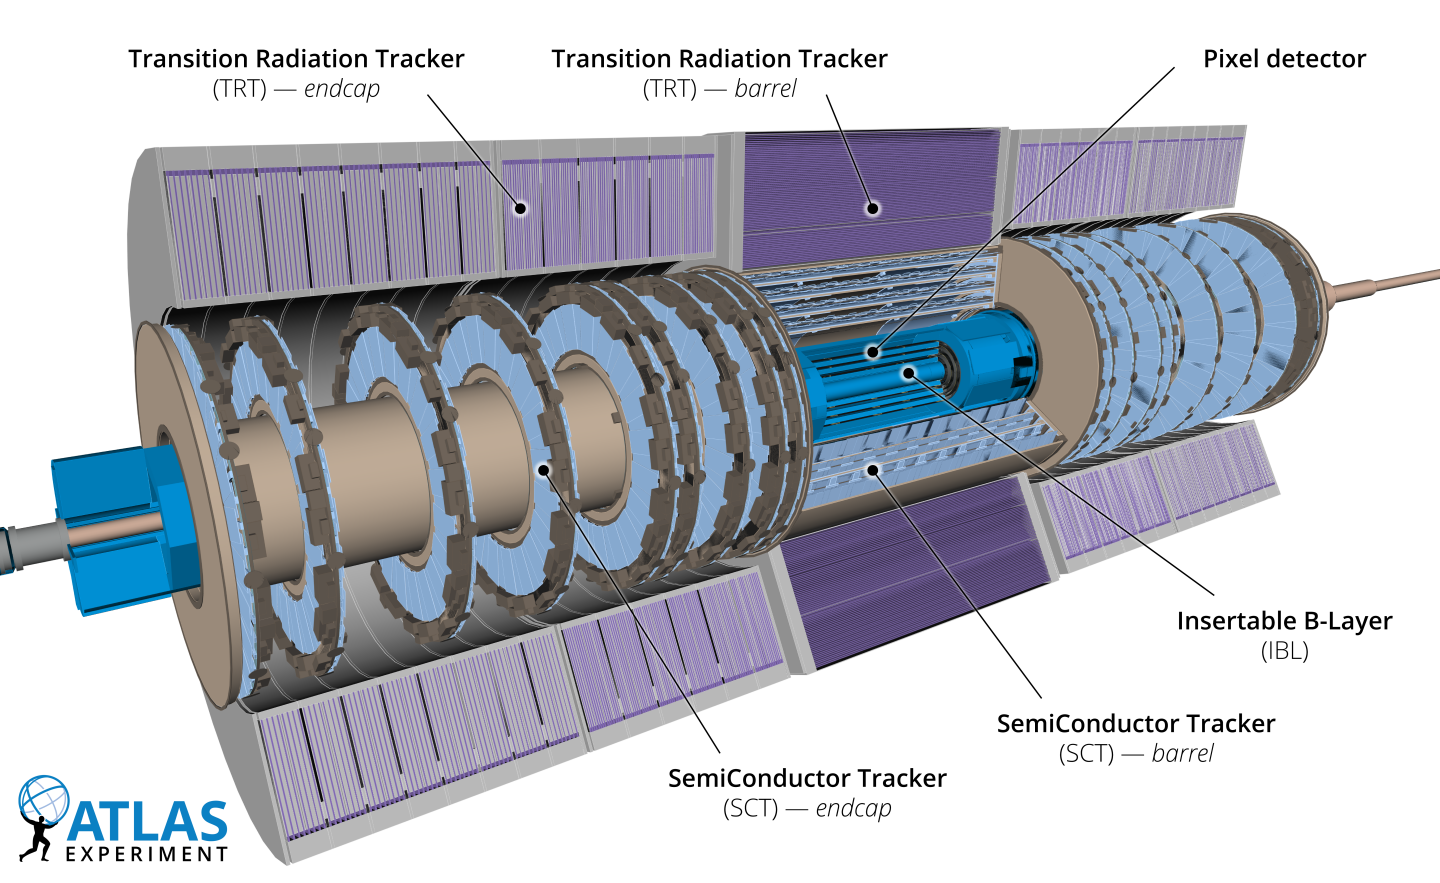
\includegraphics[width=0.59\textwidth]{Figures/cern_atlas/BetterID.png}
    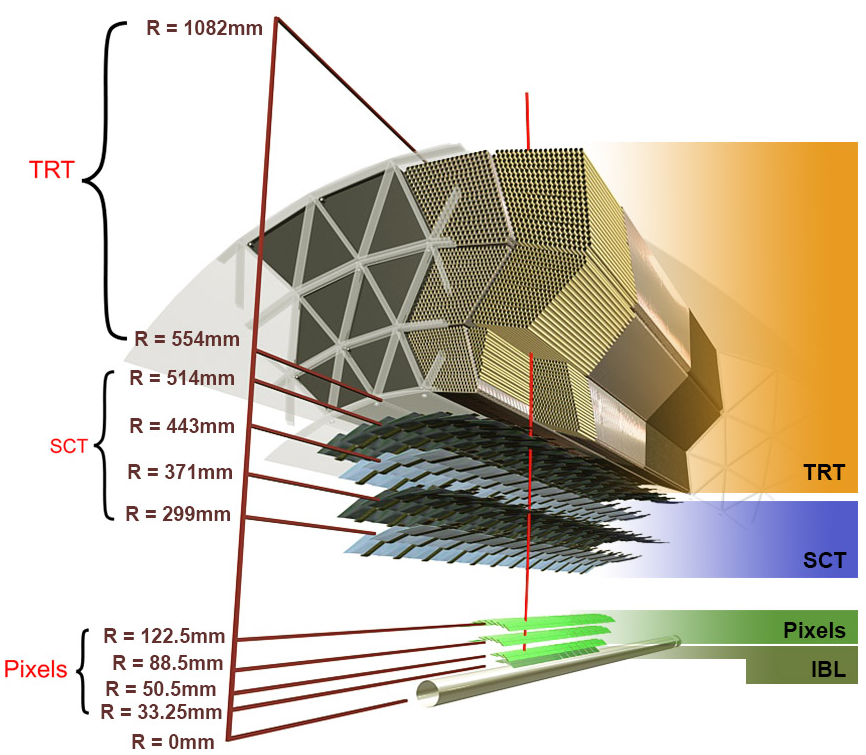
\includegraphics[width=0.39\textwidth]{Figures/cern_atlas/IDCut.png}
    \caption{Schematic of the full ATLAS Inner Detector (left) and a cross-section of the barrel region (right). Images taken from Refs.~\cite{ATLASRun3,IBLPhotos}.}
    \label{fig:atlas_inner_detector}

\end{figure}

\subsubsection{Pixel Detector}

The high-granularity silicon pixel detector~\cite{ATLASPixel} covers the innermost region of the ID.
It measures 1.4 m long and is fully contained in a diameter of 0.5 m.
High granularity is required at this scale to resolve the numerous tracks that pass through it.
Individual silicon pixels are about $50~\um$ wide in the transverse direction and about $400~\um$ long in the longitudinal direction.

Each pixel has a slight potential difference applied across it.
Ionizing radiation left by a traversing charged particle generates electron-hole pairs that drift and are collected at the p-n junctions, providing a signal.
The pixel detector has 1744 modules, each containing around 46k pixels, resulting in 80M readout channels.
These are arranged in three barrel layers placed at a radius of $50.5~\mm$, $88.5~\mm$, and $122.5~\mm$ from the beamline, with four end-cap disks on each side.

Between Run 1 and 2, an additional layer was added at a radius of $33~\mm$ to the beamline, known as the Insertable B-Layer (IBL)~\cite{ATLASIBL}.
Pixels in the IBL measure $50~\um$ in the transverse direction and $250~\um$ in the longitudinal direction.
This layer improved the $\pt$ resolution of the detector by close to 30\% for low $\pt$ tracks.
Furthermore, the enhanced $z$-resolution improved impact parameter resolution and cluster separation, allowing for better reconstruction of primary and secondary vertices.

\subsubsection{Semiconductor Tracker}

The Semiconductor Tracker (SCT)~\cite{ATLASSCT} surrounds the Pixel Detector, occupying the region between $299~\mm$ and $514~\mm$ from the beamline.
It comprises four concentric barrel layers with nine disks at each end-cap covering the region $|\eta| < 2.5$.
Like the pixel detector, the SCT is composed of silicon readout channels. Unlike the pixels, each microstrip measures $20~\um \times 12~\cm$ and thus only has high granularity in a single direction, oriented to the transverse momentum.
To improve longitudinal resolution, each SCT layer includes two back-to-back microstrip layers, rotated by $40 \unit{\milli\radian}$ relative to each other.
The SCT in total has around 6.3M readout channels.

\subsubsection{TRT}

The outermost sub-detector of the ID is the Transition Radiation Tracker (TRT)~\cite{ATLASTRT}.
It is a straw-tube tracker that aids in the momentum measurement and provides information for particle identification for tracks within $|\eta| < 2.0$.
The TRT provides the most hits per track, around 35 on average, of the three sub-detectors.
At a greater distance from the beamline, it also does not require such fine spatial resolution as the silicon detectors to provide a good measurement of the track kinematics.

It comprises approximately 300k thin-walled drift tubes, each $4~\mm$ in diameter
The barrel region contains 50k tubes, each $144~\cm$ long, while the end caps contain 250k tubes, each $37~\cm$ long.
A potential difference exists between the tube walls and an axial wire.
When a charged particle intersects the tube, it ionizes the predominantly argon gas inside, and the resulting electrons drift towards the wire, providing the signal.
There is no information on where the ionization occurred along the length of the tube.
Thus, resolution for the barrel region is only defined in the $r-\phi$ plane, and for the end-cap, it is only defined for $z-\phi$.
A polymer foil is placed between the tubes to generate transition radiation, the pattern of which allows discriminating between electrons and pions.

\subsection{Calorimeters}

ATLAS has three calorimeter systems outside the central solenoid magnet, which measure the energies of particles produced by the collisions.
Each calorimeter is designed with alternating layers of absorber and active materials.
Particles interact with the absorbers, lose energy, and produce showers of secondary particles that ionize the active material, which can be converted into a measurable signal.
These layers are typically arranged in an accordion-like structure to ensure homogenous coverage.
Different absorber materials are used to optimize the interaction and thus containment of the showers for different particle types.

The Electromagnetic Calorimeter (ECal) is specialized for measuring the energies of electrons and photons.
Surrounding this is the Hadronic Calorimeter (HCal), which is designed to measure the energies of hadrons.
These subsystems cover the region $|\eta| < 3.2$.
In addition, there is also the forward calorimeter subsystem, which measures the energy of particles in the range $3.2 < |\eta| < 4.9$.
However, information from this subsystem is not used in this work, and it is omitted from the following descriptions.
A schematic of the calorimeter systems is shown in \Cref{fig:atlas_calorimeters}.

\begin{figure}[htb]
    \centering
    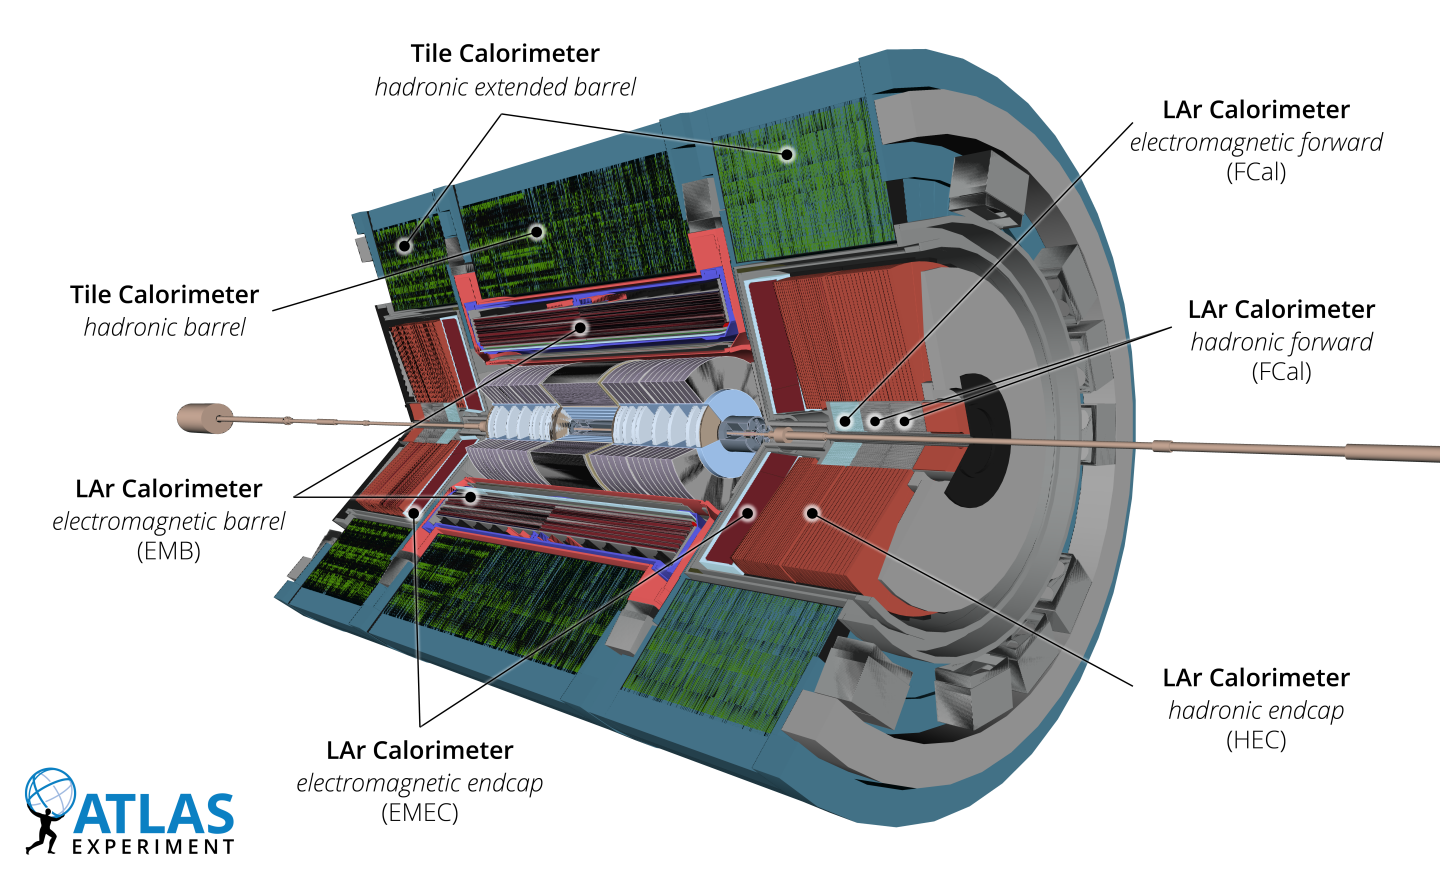
\includegraphics[width=0.99\textwidth]{Figures/cern_atlas/Calos.png}
    \caption{Schematic of the ATLAS calorimeter systems. Image taken from Ref.~\cite{ATLASRun3}.}
    \label{fig:atlas_calorimeters}
\end{figure}

\subsubsection{Electromagnetic Calorimeter}

The Cal~\cite{ATLASECal} is a high granularity calorimeter which uses liquid argon as the active material and lead as the absorber.
To keep the argon in a liquid state, the ECal is cooled to $-185~\unit{\degree C}$.
These materials are chosen to optimize the containment of electromagnetic showers produced by electrons and photons, via pair production and bremsstrahlung radiation, while minimising the energy loss of heavier particles.
The barrel ECal covers the range $|\eta| < 1.475$ and is split into three layers, decreasing in granularity with distance from the beamline.
The inner layer allows for more precise shower measurements which assists in the identification of pions.
The Liquid Argon Electromagnetic Enc-Cape (EMEC) and covers the range $1.375 < |\eta| < 3.2$.
Unlike the ID, the ECal resolution increases with incident particle energy.

\subsubsection{Hadronic Calorimeter}

The HCal or Tile Calorimeter~\cite{ATLASHCal} encompasses the ECal and is designed to measure the energies of hadrons.
It uses steel as the absorber and scintillating tiles as the active material made from polystyrene.
The hadrons are contained by losing energy through inelastic nuclear interactions with the steel, producing a shower of electrons and photons which are detected by the tiles.
In the forward regions of the calorimeter, $1.5 < |\eta| < 3.2$, a copper/LAr combination is used.
The granularity and energy resolution of the HCal are lower than the ECal.

\subsection{Muon Spectrometer}

Other than neutrinos, which traverse the entire detector without interacting, muons are the only particles that easily penetrate through the calorimeters, incurring minimal energy loss.
Though they leave tracks in the ID, the Muon Spectrometer (MS)~\cite{ATLASMuon,ATLASRun3} provides triggering information, identification, and extra momentum measurements for muons.
The MS is the outermost sub-detector of ATLAS and is shown in \Cref{fig:atlas_muon_spectrometer}.
Its systems are arranged in three barrel layers covering $|\eta| < 1.2$ and several end-cap layers or wheels covering $1 < |\eta| < 2.7$.
The wheels are placed on either side of the detector at a distance of $7.4$~m, $14$~m, and $21.5$~m from the IP.

Monitored Drift Tubes are the spectrometer's primary tracking component and are similar in principle to the straw tubes in the TRT@.
More than 380k aluminum tubes, each with a diameter of $30$~mm and primarily filled with argon gas, are organized into three barrel layers and four end-cap disks.
In addition, Cathode Strip Chambers are used in inner layers of the end-cap to cope with the higher particle flux.
These are multi-wire proportional chambers built into strips.

Three large air-core toroidal magnets generate the magnetic field in the MS\@, one in the barrel region and one in each end-cap regions.
Each magnet has eight coils and deflects the muons, allowing for the measurement of their momentum.

\begin{figure}[htb]
    \centering
    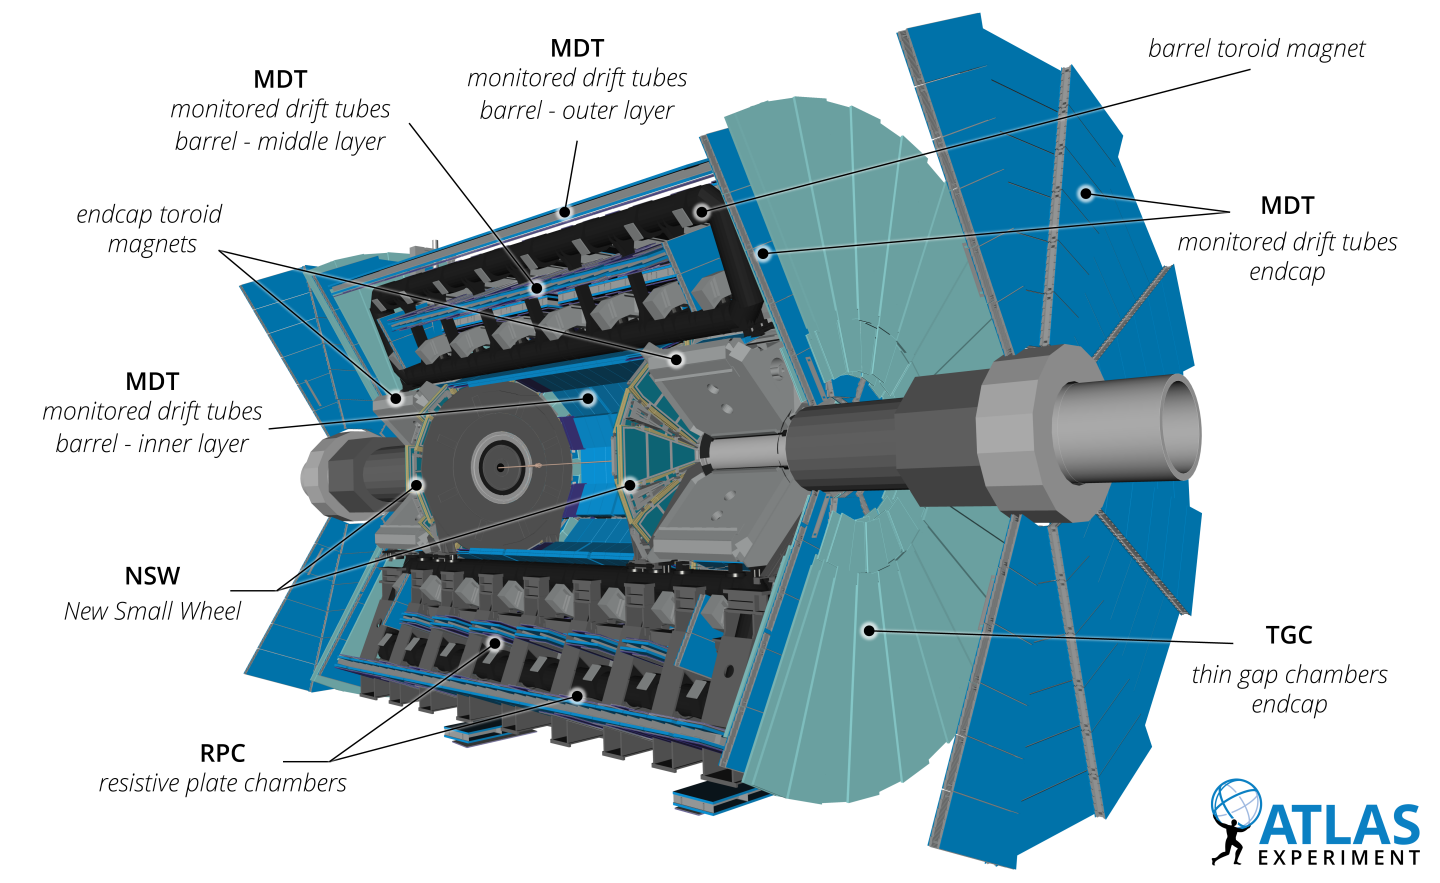
\includegraphics[width=0.99\textwidth]{Figures/cern_atlas/MS.png}
    \caption{Schematic of the ATLAS Muon Spectrometer. Image taken from Ref.~\cite{ATLASRun3}.}
    \label{fig:atlas_muon_spectrometer}
\end{figure}

\section{Reconstruction}
\label{sec:event_reconstruction}

Reconstruction is the process of converting the raw detector signals into collections of defined physical objects to better understand the collision events.
This process is performed offline, after the data has been recorded and stored, and uses information from all sub-detectors.

This section describes the basics of track, vertex, and jet reconstruction at ATLAS, as well as several approaches to jet tagging.

\subsection{Tracks}

Track reconstruction refers to taking the collection of hits registered by the ID, and grouping them into individual tracks likely to have been produced by a single charged particle.
Tracks are key ingredients in the reconstruction and identification of other particles, such as electrons and muons, jets, and the multiple vertices produced in each collision.
A full description of the track reconstruction pipeline used for ATLAS Run 2 data can be found in Ref.~\cite{PerformanceATLASTrack}.
Track reconstruction is performed in nuerous stages.
Hits are first clustered into space points, after which iterative track-finding algorithms are used, followed by cleaning and ambiguity resolution.

\subsubsection{Clusterization}

A single particle may deposit energy in multiple adjacent pixels or strips in the ID\@.
This is due to the drift of electrons between sensors within the solenoid magnetic field or from the incident angle of the particle.
These hits are first combined into clusters which are then used to form \textit{space points} (SP) defined in three dimensions.
For the SCT, these clusters also combine information from the two back-to-back layers.
Position uncertainties of these points are estimated from cluster sizes and detector geometry.
In dense environments the clustering algorithm may merge mistakenly merge hits from different particles, leading to a higher rate of fake tracks.

\subsubsection{Track Seeding}

Tracks are \textit{seeded} by grouping triplets of SPs in three sequential layers in either the pixel or SCT subdetectors.
Each of these seeds forms a \textit{track candidate} and are used to determine the first crude estimates of the track parameters, assuming a perfectly uniform magnetic field and helical trajectory.
The only requirement to improve purity is that one additional SP is found compatible with the track candidate outside the seeding region.

A combinatorial Kalman filter~\cite{ApplicationKalmanFiltering} is employed to iteratively extend this candidate by incorporating additional SPs in the other layers both towards and away from the IP\@.
If multiple compatible space-point extensions are found on the same layer, the filter generates several track candidates for each seed.
At this stage, hits may be shared between multiple candidates, which is intentionally done to maximize the number of possible candidates and thus the efficiency of the algorithm.

The following steps are designed to improve the track quality and remove fake tracks.

\subsubsection{Ambiguity Resolution}

The ambiguity resolver begins by defining a \textit{track score} for each candidate.
This score quantifies the likelihood that each candidate corresponds to a real trajectory.
The score takes into account several factors; the number of SP assigned to the track will increase its score, while the number of holes will decrease it.
Holes are defined as intersections between the reconstructed track and active sensor material where no matching SP is found.
They can be found in data due to inefficiencies in the silicon sensors.
The track score also considers the $\chi^2$ of the track fit.
Tracks with higher \pt also receive a higher score.
The ambiguity resolver then iterates over the list of track candidates in order of decreasing score.

Clusters can overlap naturally in high-density environments.
These are referred to as \textit{merged clusters}.
A neural network estimates the number of particles traversing each cluster and their positions~\cite{NeuralNetworkClustering}.
This information allows the cluster to be split and allocated to the different candidates.
A track can have no more than two shared clusters, and clusters may be shared by no more than two tracks, with preference given to the track with the highest score.
The refined and purified track candidates are then re-fit to obtain the final parameters.
It obtains a new score and is inserted back into the list of candidates.

During this stage, seeds that fail the track-finding process are checked for compatibility with information from the calorimeter.
If a seed is within a region of interest in the calorimeter, the track-finding procedure is repeated, permitting an extra \textit{kink} in the track as this may have been caused by Bremsstrahlung radiation.
This step improves electron reconstruction efficiency.

The ambiguity resolver fully rejects track candidates if they fail to meet the criteria in \Cref{tab:track_criteria}.
If the track is processed twice by the resolver without modification, it is saved to the final collection and all associated hits are removed.

\begin{table}[h!]
    \centering
    \begin{tabular}{ll}
        \toprule
        Parameter           & Selection   \\
        \midrule
        $p_T$               & $> 400$ MeV \\
        $|\eta|$            & $< 2.5$     \\
        $|d_0|$             & $< 3.0$ mm  \\
        $|z_0 \sin \theta|$ & $< 5$ mm    \\
        Shared clusters     & $< 2$       \\
        SCT + Pixel hits    & $\geq 8$    \\
        Pixel holes         & $< 2$       \\
        SCT + Pixel holes   & $< 3$       \\
        \bottomrule
    \end{tabular}
    \caption{Track selection criteria used by the ambiguity resolver.}
    \label{tab:track_criteria}
\end{table}

\subsubsection{TRT Extension}

Finally, information from the TRT is used to extend the tracks.
A similar Kalman filter incorporates TRT hits starting from the predicted intersection between each silicon track and the TRT.
If successful, the TRT hits are added to the track, and the whole track is fit once more using a global $\chi^2$ fitter.
The inclusion of TRT hits enhances momentum resolution and allows for particle identification.
However, the extension may be rejected if it worsens the $\chi^2$ of the track candidate or if more than 50\% of the TRT hits are tube hits with no leading edge.

\subsection{Vertices}

Vertex reconstruction is the process of identifying the many primary and secondary vertices produced in each collision.
Each vertex is a location in space, constructed from a convergence of fully reconstructed tracks, and indicates the point of origin for multiple charged particles.

Primary vertices are those produced by the many $pp$ collisions during the bunch crossing.
For Run 1 and 2, the primary vertices are reconstructed using the Iterative Vertex Fitter~\cite{ATLASVertex}.
First, a seed position of the vertex is selected using the mode of the $z$-coordinate all tracks in the event measured at the point of closest approach to the beamline.
Next, the vertex position is iteratively refined, and in each iteration, less compatible tracks are down-weighted.
After the final iteration, all tracks with low enough weights are removed from the vertex and used for the next.

For each event, the primary vertex with the highest $\Sigma\pt^2$ of all associated tracks is labelled as the \textit{hard scatter vertex}.
It is sometimes ambiguously referred to as \textit{the} primary vertex (PV) while the others are referred to as \textit{pileup} vertices.
Reconstruction on Run 3 data is switching to an Adaptive Multi-Vertex Fitter~\cite{Run3Vertex}.

Secondary vertices are those produced by the decay of particles originating from the PV.
This secondary decay must take place at a distance sufficiently far away in the transverse plane to be resolved and not mistakenly identified as pileup.
They are typically caused by the decay of long-lived $b$-hadrons or the interaction of particles with the detector material and are thus crucial tools for identifying $b$-jets.
In ATLAS, secondary vertex reconstruction is performed within the context of jet reconstruction using the JetFitter~\cite{JetFitter} or SV1~\cite{SV1} algorithms.

\subsection{Jets}
\label{sec:jets_reconstruction}

As described in \Cref{sec:jets} are an emergent property of QCD\@, which results in a collimated spray of particles stemming from the decay and fragmentation of an initiating color-charged parton.
From a detector perspective, jets result in large localized energy deposits in both calorimeters and many tightly packed tracks in a cone emanating from the PV.
The width of the jet cone is dependent on the mass of the initiating particle and its transverse momentum, with $\Delta R \approx \sfrac{2m}{\pt}$.

Due to the stochastic nature of the showering process, the jet signal can never be perfectly isolated.
Particles within the jet cone may overlap with other initial state radiation, multiple parton interactions (from the underlying event), or pileup.
Jet reconstruction is, therefore, a difficult optimization problem.
The goal is to maximally capture the energy of the initiating particle while minimizing the contamination from other sources.
A jet reconstruction algorithm should capture all hard partons in the event, have an axis parallel to the jet momentum, and accept roughly uniform contamination.

Jet reconstruction in ATLAS is performed using the anti-$k_t$ algorithm~\cite{AntiKt}.
This is a sequential recombination algorithm that iteratively clusters a collection of objects.
It is both infrared and collinear safe.
The algorithm is defined by a maximum distance parameter $R$.
The algorithm begins with the hardest, highest \pt, object in the event $i$.
During each iteration, the distance $d_{ij}$ is calculated to all other objects $j$ in the event,
\begin{equation}
    d_{ij} = \frac{1}{\max(\pt{_i}^2, \pt{_j}^2)} \frac{\Delta R_{ij}^2}{R^2}.
\end{equation}
If this value is less than $\sfrac{1}{\pt{_i}^2}$, then the objects are combined, and the algorithm proceeds; otherwise, $i$ is considered a jet and removed from the list.
The algorithm continues until all objects are clustered or declared as jets.

Jets can be clustered using the anti-$k_t$ algorithm with a variety of inputs.
During Run 1, jets were constructed from topo-clusters, topologically connected calorimeter cells~\cite{TopoJets}.
In some analyses, jets are clustered from tracks only~\cite{TrackJets}.
The general approach for Run 2 and 3 data is to include both sets of information using the Particle Flow (PFlow) algorithm~\cite{PFlow}.

\subsubsection{Particle Flow}

The PFlow algorithm is designed to prevent the double-counting of momentum contributions from charged particles that leave both ID tracks and calorimeter energy deposits.
This algorithm iterates through the tracks in descending \pt order, constructing charged PFlow objects.
The algorithm begins by attempting to match the selected track to a topo-cluster in the calorimeter.
Both are then used to compute the expected energy contribution to the cluster by the particle that created the track.
A single particle may deposit energy in multiple topo-clusters, and the algorithm evaluates the probability of this occurring and may include additional topo-clusters if necessary.
The expected energy is then subtracted from the associated topo-clusters, cell-by-cell.
A new track is then selected, and the process is repeated.
If, at any point, the remaining cell energy following the subtraction falls below expected shower fluctuations, it is removed.

Topo-clusters not matched to any tracks are deemed to have been produced from neural particles and left unmodified.
These, and the remaining clusters after the subtraction step, are used to construct neutral PFlow objects.

The output of the PFlow algorithm is a collection of charged and neutral PFlow objects, each with defined energy and momentum.
Charged PFlow objects not matched to the PV are removed to reduce pileup contamination.
The remaining objects are clustered into jets using the anti-$k_t$ algorithm with $R=0.4$.

\subsubsection{Jet Association}

Once jets are defined, other objects can be associated using a $\Delta R$ matching criterion.
For instance, a jet might be constructed from calorimeter energy deposits, but tracks can still be associated.
The width of the $\Delta R$ association cone typically decreases as with jet \pt.
This track association is beneficial for the ATLAS experiment because it enables using the Jet Vertex Tagger (JVT)~\cite{JVT}.
The JVT leverages the transverse momenta from associated tracks to discriminate against jets originating from pileup interactions.
Furthermore, many of the flavour tagging algorithms mentioned in the next section and in \Cref{sec:flavour_tagging} operate on the set of tracks associated with a jet, even though the jets themselves were clustered from PFlow objects.

\subsection{Large Radius ``Fat'' Jets}

Many decay channels of massive particles result in multiple parton final states.
Some examples that are frequently encountered include $W/Z \rightarrow q \bar{q}$, $t \rightarrow Wb \rightarrow q \bar{q} b$, and $H \rightarrow VV \rightarrow q \bar{q} q \bar{q}$.
If the initiating particle is produced at rest in the lab frame, the final state partons would be emitted back-to-back and likely be reconstructed as individual jets.
However, as the transverse momentum of the initiating particle increases, the decay products become more collimated, as shown in \Cref{fig:jet_topologies}.
In the highly boosted regime, the parton showers overlap in the detector and may be reconstructed as a single jet.
To fully capture these composite jets, the anti-$k_T$ algorithm is run with a larger radius parameter of $R=1.0$.
These jets are colloquially referred to as \textit{fat} jets.

The overlapping showers lead to a distinct internal substructure within the jet, with regions of high energy density called \textit{subjets} or \textit{prongs}.
The processes listed above, for example, would lead to 2-prong, 3-prong, and 4-prong jets, respectively.
Jets from non-resonant QCD processes tend to have smooth energy distributions and no substructure (1-prong).

\begin{figure}[htb]
    \centering
    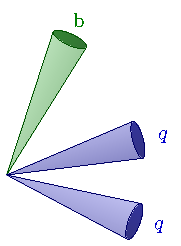
\includegraphics[width=0.28\textwidth]{Feynman/sep.pdf}
    \hfill
    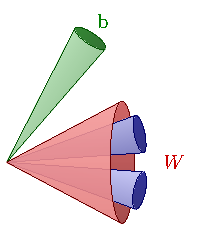
\includegraphics[width=0.28\textwidth]{Feynman/W.pdf}
    \hfill
    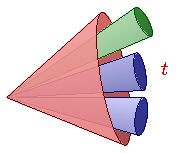
\includegraphics[width=0.28\textwidth]{Feynman/top.pdf}
    \caption{A top quark decay with increasing momentum, showing the transition from three separately resolved jets (left), to a $W$-jet and a $b$-jet (middle), to a single fat jet (right).}
    \label{fig:jet_topologies}
\end{figure}

The number of subjets and the angular separation of these subjets can be used to identify the initiating particle.
One commonly used set of observables to describe jet substructure is its \emph{N-subjettiness}~\cite{Subjet}, denoted by ${\tau_N}$.
N-subjettiness is a measure of how well a jet can be decomposed into $N$ subjets.
For a given $N$ these subjets can be found via some other clustering algorithm, such as the exclusive-$k_t$ algorithm~\cite{ExclusiveKT}, and then the $\tau_N$ observable is defined as,
\begin{equation}
    \tau_N = \frac{1}{\pt R} \sum_{i} \min(\Delta R_{1,i}, \Delta R_{2,i}, \ldots, \Delta R_{N,i}),
\end{equation}
where $k$ runs over the constituents of the jet, and $\Delta R_{i,j}$ is the angular separation between the $i$th constituent and the $j$th subjet.
The discriminating variable for jet tagging is often the ratio of these observables, $\tau_{21} = \sfrac{\tau_2}{\tau_1}$, is commonly used to distinguish vector boson jets from QCD jets, and
$\tau_{32} = \sfrac{\tau_3}{\tau_2}$, is used to identify top quark jets.

Other commonly used observables relate to the jet's energy correlation functions~\cite{ECF} and their ratios.
Analyses at ATLAS make frequent use of the $\Dtwo$ observable~\cite{ATLASD2} to separate 1-prong and 2-prong jets,
\begin{align}
    \Dtwo & = \frac{e_3}{(e_2)^3}, \\
          & = \frac{
        \sum_{1 \leq i < j < k \leq N} z_i z_j z_k \Delta R_{ij} \Delta R_{ik} \Delta R_{jk}
    }{
        (\sum_{1 \leq i < j \leq N} z_i z_j \Delta R_{ij})^3
    },
\end{align}
where $z_i$ is the \pt fraction of the jet carried by the $i$th constituent, and $\Delta R_{ij}$ is the angular separation between the $i$th and $j$th constituents, and $N$ is the number of constituents in the jet.
Additionally, the Energy Flow Polynomials~(EFPs)~\cite{EFP} are a set of basis features which are sensitive to the underlying substructure of different jet types.

\subsection{Heavy-Flavour Tagging}
\label{sec:flavour_tagging}

Heavy-flavour tagging, or simply flavour tagging, is the process of identifying jets that contain the decay products of $b$-quarks ($b$-jets) or  $c$-quaks ($c$-jets).
Jets originating from the decay of $u-$, $d-$, $s-$ quarks and gluons are collectively called light-jets.
Identifying jets from either process is known as $b$-tagging or $c$-tagging, respectively.
In ATLAS, $b$-tagging plays a critical role in many analyses, particularly those measuring properties of the Higgs boson or the top quark.
Nearly all top quarks decay rapidly into a $W$-boson and a $b$-quark, and the dominant decay mode of the Higgs boson is to a pair of $b$-quarks.

Unlike the methods to distinguish large-radius jets, which rely on the jet substructure, the main distinguishing feature used in $b$-tagging is the extended lifetime of hadrons containing $b$-quarks.
As discussed in \Cref{sec:electroweak}, the weak interaction CKM matrix is nearly diagonal, thus favouring transitions within the same generation.
However, the $b$-quark is approximately 40 times lighter than the $t$-quark; it can only decay into lighter generations and is thus CKM suppressed.

The $b$-hadrons are quasi-stable bound states between a $b$-quark and one or two lighter quarks.
They have an average lifetime of around $1.5~\ps$, and if emitted with $\pt=50~\GeV$ would travel around $L_{xy} = 5~\mm$ in the transverse plane before decaying.
This distance can be resolved by the ID vertex fitting algorithms and would result in a vertex with a notable transverse displacement, as shown in \Cref{fig:btagging}.
The presence of a high mass secondary vertex within a jet is the primary feature used in $b$-tagging

\begin{figure}[htb]
    \centering
    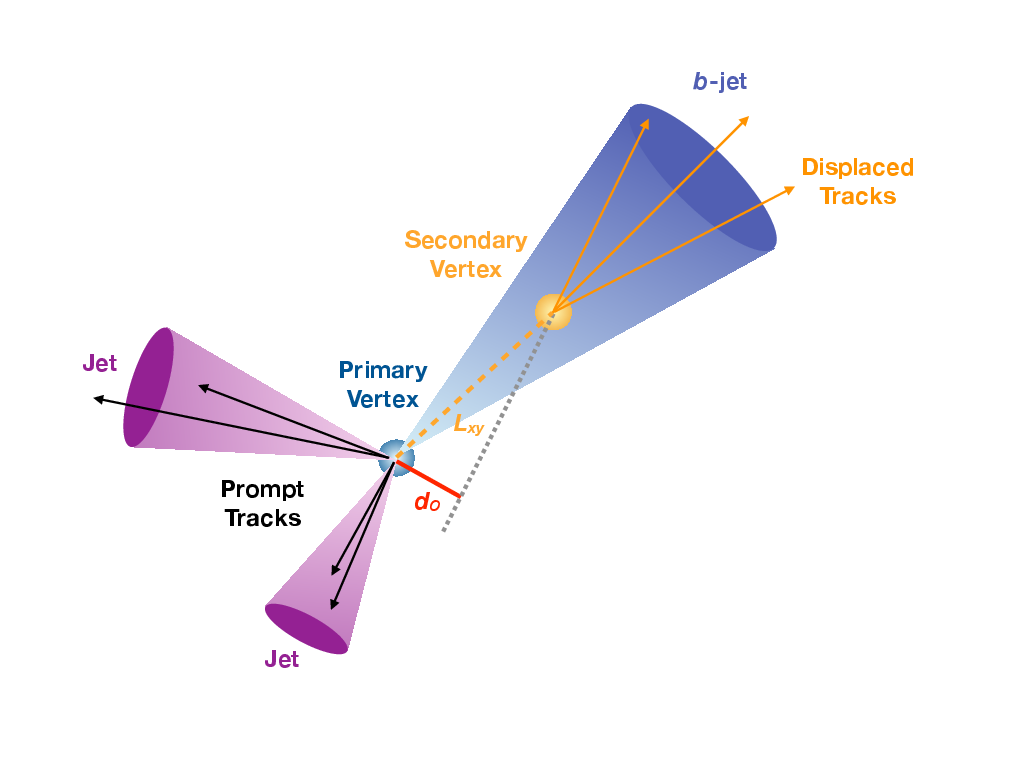
\includegraphics[width=0.75\textwidth]{Figures/cern_atlas/bjet.png}
    \caption{An interaction producing two light-flavour jets and one $b$-jet in the transverse plane. $B$-hadrons have a transverse decay length $L_{xy}$ of a few millimetres, creating displaced tracks and a secondary vertex. The transverse impact parameter (d0) is the closest approach distance of these tracks to the primary vertex, typically large for b-hadrons. Image taken from Ref.~\cite{BJetImage}.}
    \label{fig:btagging}
\end{figure}

Flavour tagging at ATLAS has evolved over many years.
Typically, the tools return the likelihood of a $b$- $c$- or light-jet, given some properties of the associated tracks.
A collection of comparisons between these algorithms used in $b$-tagging is shown in \Cref{fig:btagging_roc}.
Several handcrafted algorithms were designed for flavour tagging before the start of Run 1, such as IPxD~\cite{IPxD}, SV1~\cite{SV1}, and JetFitter~\cite{JetFitter}.
Each tagger used a unique approach to extract different high level features from the jet and associated tracks.
They also yielded different performances depending on the phase space.
It was found that combining the most discriminating features from each in a single neural network resulted in a more versatile tagger known as MV1~\cite{MV1}, which was used at the start of Run 1.
At the start of Run 2, it was replaced by MV2~\cite{MV2}, a boosted decision tree with similar inputs.
In 2017, it was replaced by DL1~\cite{DL1}, a neural network again with much the same approach.
These figures plot the $b$-jet efficiency against light and $c$-jet rejection.

Also introduced at this time was the first tagger based purely on the raw collection of tracks and their parameters, known as RNNIP~\cite{RNNIP}.
This was a recurrent neural network (RNN) that processed all the tracks in the jet sequentially to determine the three class probabilities.
Again, the performance could be improved by combining the outputs of RNNIP with the other IPxD, SV1, JetFitter.
This combination yielded the DL1r tagger~\cite{Run2FTAlgs}.
A second track-based tagger known as DIPS~\cite{DIPS} was developed in 2020.
It used the deep sets architecture~\cite{DeepSets}, and the corresponding combined tagger was labelled DL1d~\cite{AlexThesis}.

The most recent iteration is a departure from the previous approach of combining multiple high level and track based taggers.
In 2022 ATLAS introduced the GN1 tagger~\cite{GN1} which is a graph neural network, \Cref{ch:gnns}, that only uses the track information.
This single network, as shown in \Cref{fig:gn1}, simultaneously performs jet tagging, as well as vertex matching and track classification trained end-to-end.

More details on the GN1 tagger are provided in \Cref{ch:spice}, which also details the development of a new flavour tagging algorithm, GN2, which would supersede it.

\begin{figure}[h]
    \centering
    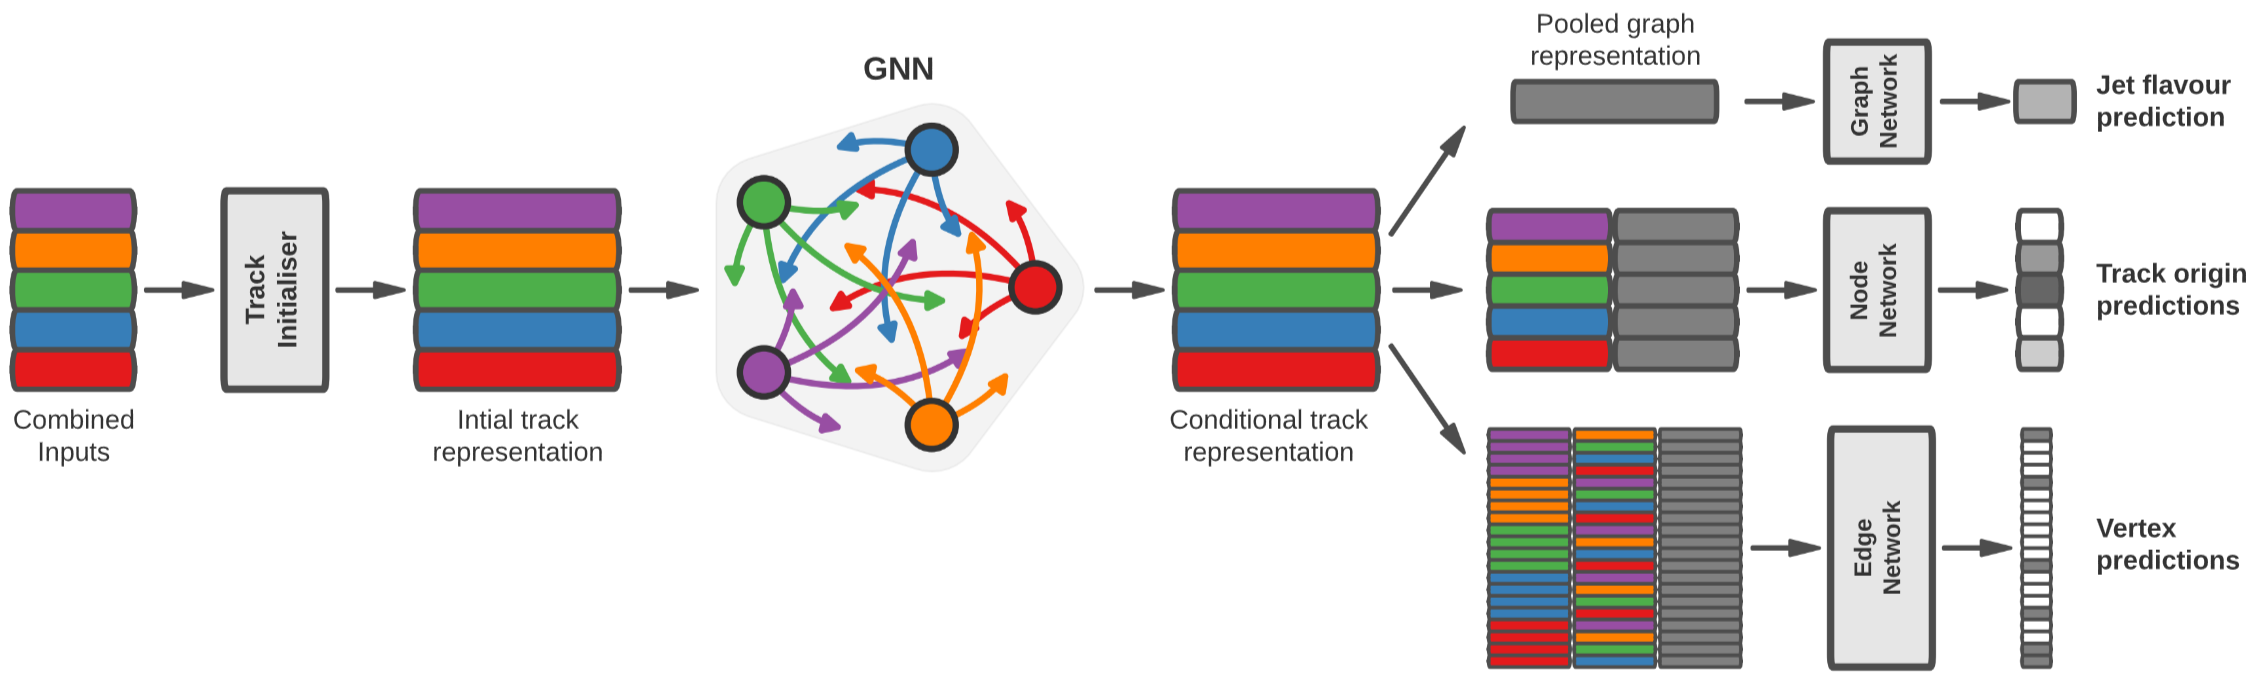
\includegraphics[width=0.99\textwidth]{Figures/cern_atlas/GN1.png}
    \caption{Schematic diagram of the GN1 model from Ref.~\cite{GN1}.}
    \label{fig:gn1}
\end{figure}


\begin{figure}[h]
    \centering
    \begin{subfigure}{0.435\linewidth}
        \centering
        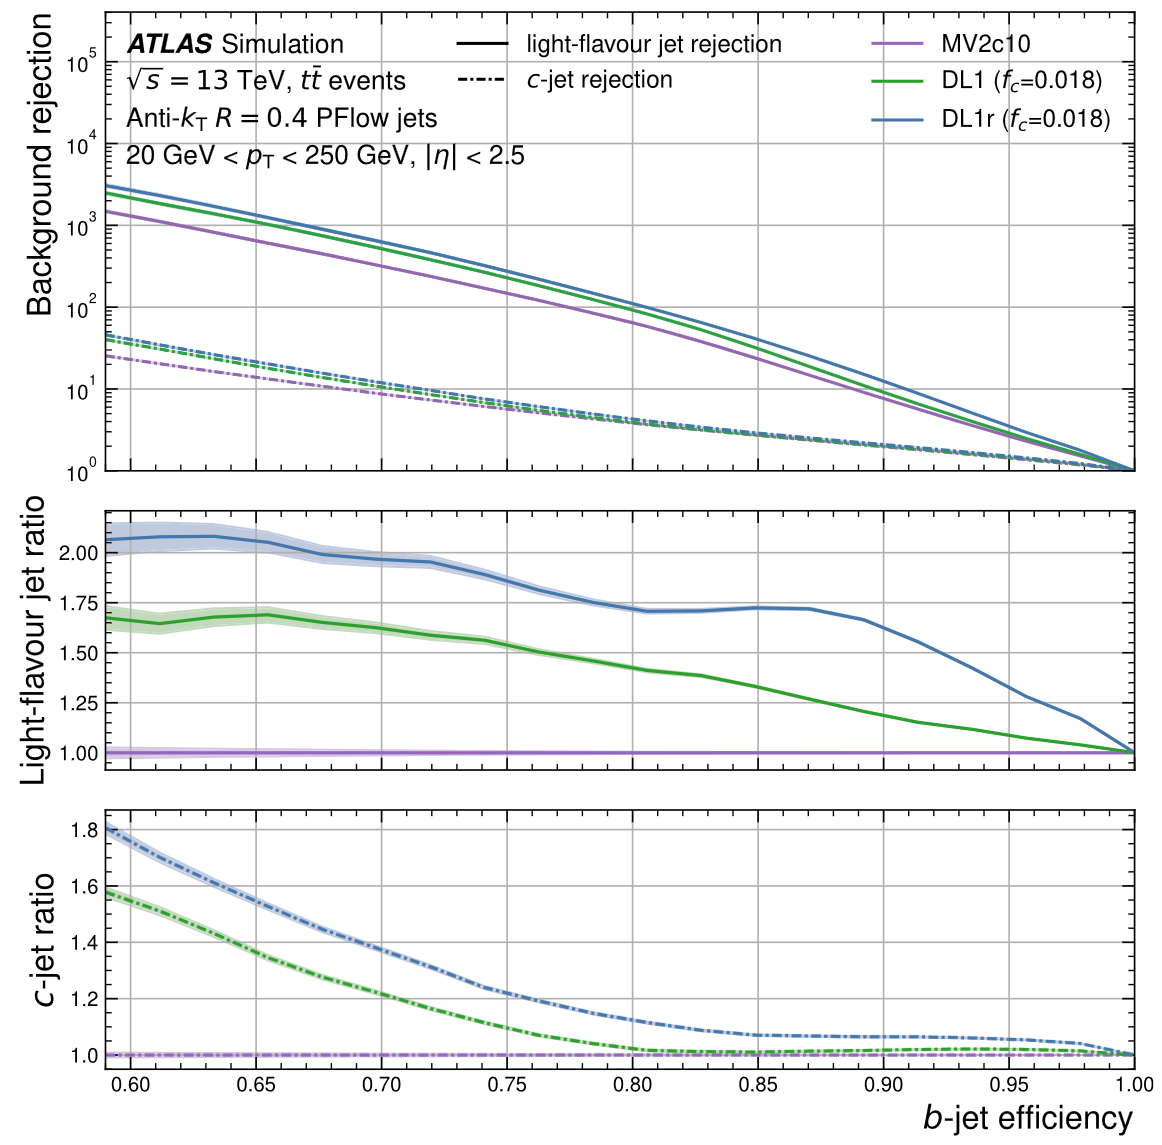
\includegraphics[width=\linewidth]{Figures/cern_atlas/dl1r.png}
        \caption{}
        \label{fig:dl1r}
    \end{subfigure}
    \begin{subfigure}{0.555\linewidth}
        \centering
        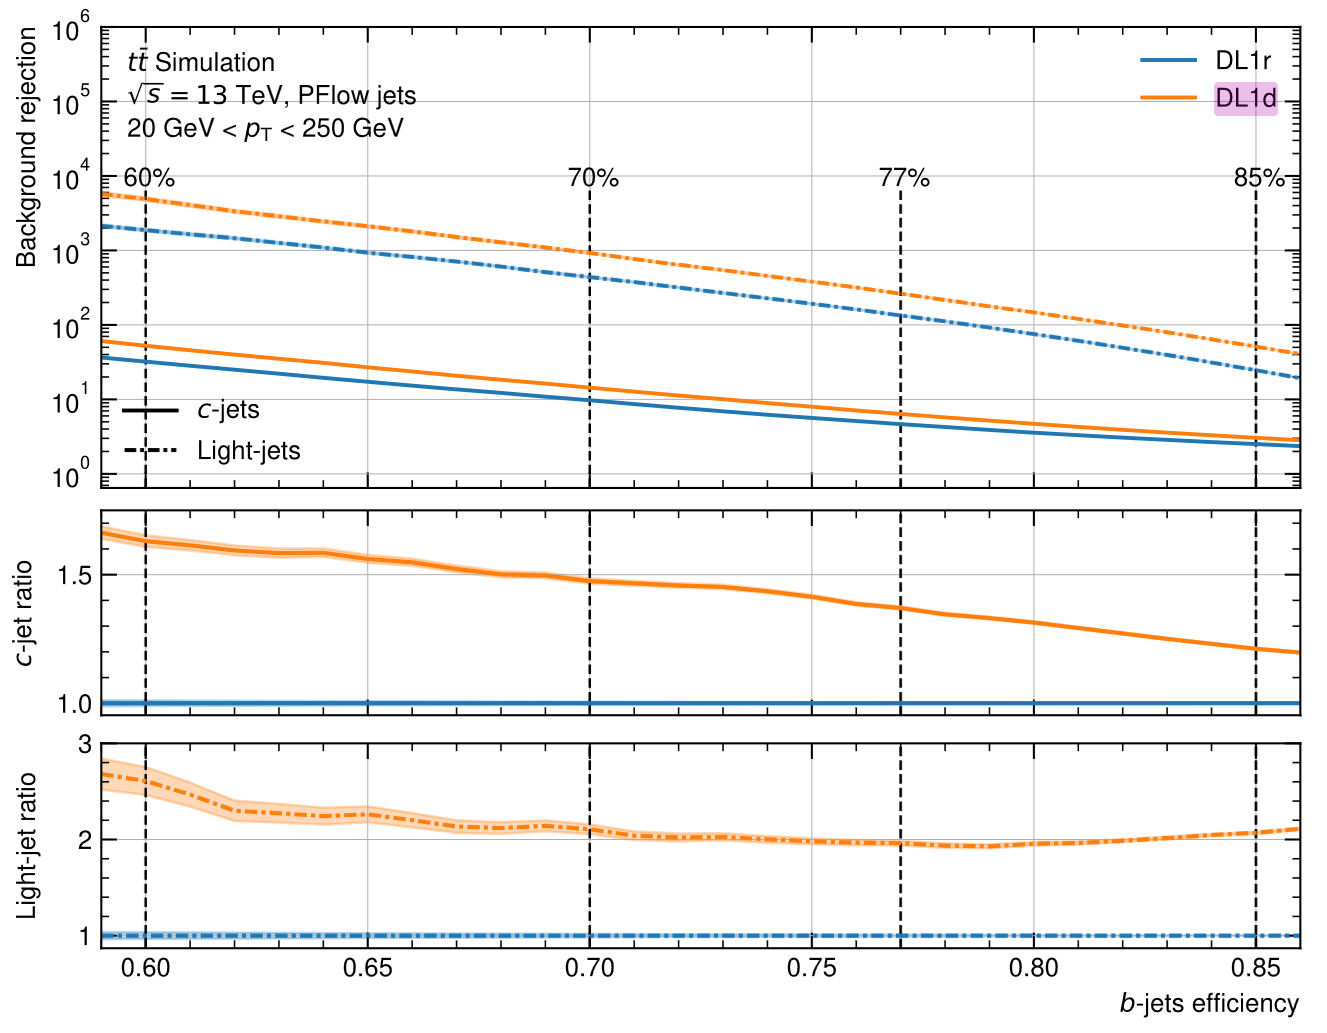
\includegraphics[width=\linewidth]{Figures/cern_atlas/dl1d.png}
        \caption{}
        \label{fig:dl1d}
    \end{subfigure}
    \begin{subfigure}{0.85\linewidth}
        \centering
        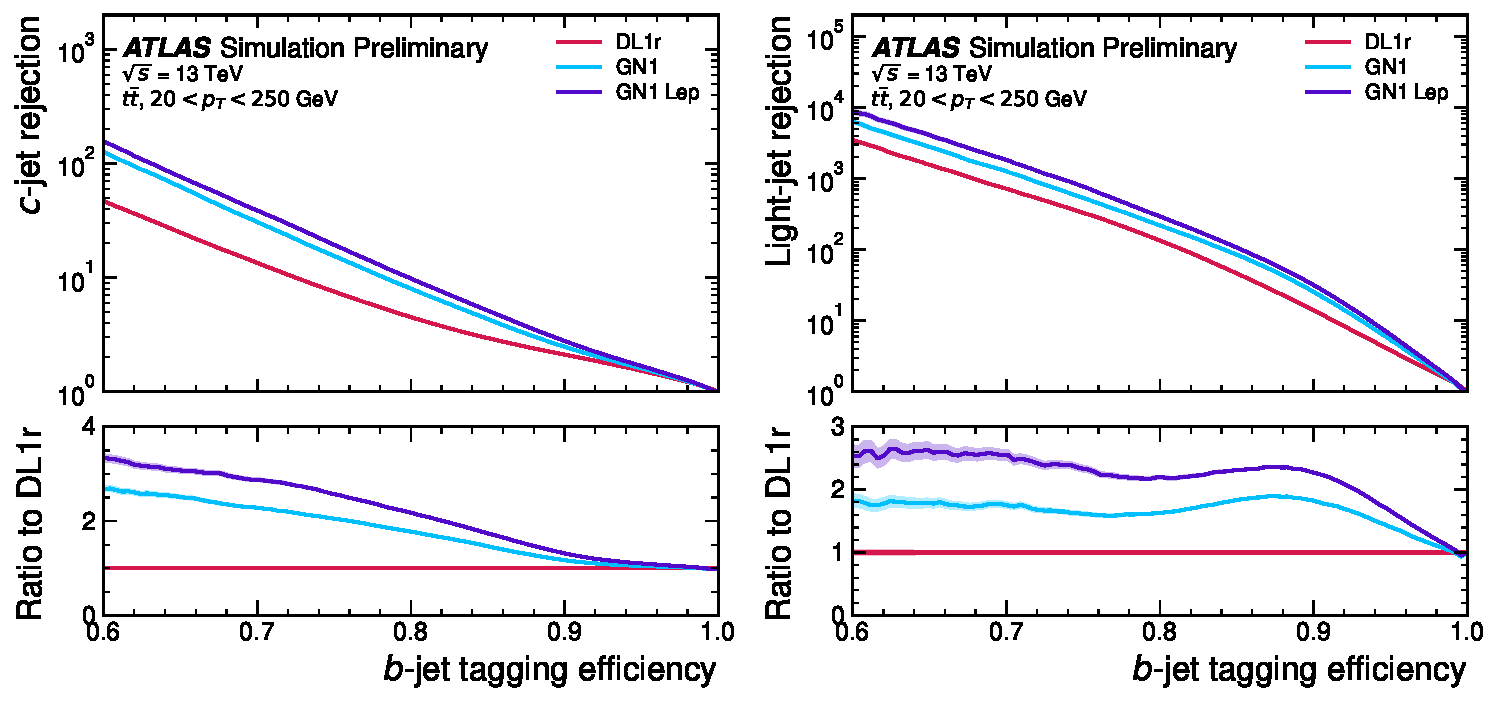
\includegraphics[width=\linewidth]{Figures/cern_atlas/gn1roc.pdf}
        \caption{}
        \label{fig:gn1r}
    \end{subfigure}
    \caption{The rejection factors for light-jets and c-jets as a function of the $b$-tagging efficiency for the different algorithms used by ATLAS over the years as measured on simulated \ttbar datasets. \subref{fig:dl1r} shows the performance of the MV2, DL1, DL1r taggers with the bottom panels showing the performance ratio to MV2. \subref{fig:dl1d} shows the performance of the DL1d and DL1r taggers with the bottom panels showing the performance ratio to DL1r. \subref{fig:gn1r} shows the performance of the GN1 tagger. Images taken from Refs.~\cite{Run2FTAlgs,AlexThesis,GN1} respectively.
    }
    \label{fig:btagging_roc}
\end{figure}

% \part{Transformers for Flavour Tagging}
% Machine learning (ML) has become a powerful tool in HEP in recent years.
ML has also been evolving rapidly, with new algorithms and techniques being developed at a breakneck pace.
The observed performance gain in many algorithms and operations used in particle physics that have adopted ML has been well documented and hard to ignore.
One of the most successful stories has been using deep learning for flavor tagging, identifying the flavor of quark that initiated a jet in the ATLAS experiment at the LHC.
However, the field of HEP has unique challenges for ML adoption, such as the requirement for explainability and robustness.
This chapter introduces relevant concepts required to understand the latest developments in the models used in flavor tagging at ATLAS: the description of deep learning, the motivation of graph neural networks, and the implementation of a transformer model.

\chapter{Deep Learning Basics}

Deep learning is the subset of machine learning that focuses on the development and training of artificial neural networks.
These neural networks take the form of a series of composable, parameterized, and differentiable transformations that map input data to output data.
Training or optimization of the network is done by modifying the parameters of each transformation to minimize some error metric over a dataset.
This is typically performed using gradient-based algorithms.
The exact form of how the loss is calculated differentiates the various types of learning, such as supervised, unsupervised, self-supervised, reinforcement, etc\footnote{There is often overlap between these categories}.

Initially, artificial neural networks were inspired by the structure of the brain, with many layers of interconnected artificial neurons processing information and sending signals to each other.
While individual neurons are simple, the emergent behaviour of the network can be complex.
As the field has evolved, the initial biological inspiration of neural networks has given way to more abstract, mathematical descriptions.
Today, network design is driven by inductive biases, computational efficiency, observations in training dynamics, and (above all) empirical results.
From this more practical perspective, an artificial neural network is long computational graph composed of differentiable operations arranged in layers that transform between collections of real-valued tensors.
The ``depth'' of a deep learning model refers to the number of layers used in the network.

The primary distinction between deep learning and other parameterized curve fitting methods is a matter of scale.
Modern networks now contain billions of parameters, requiring large datasets, specialized hardware, and sophisticated optimization algorithms to train effectively.
As the networks have grown in size and complexity, model interpretability has become a significant challenge and an active area of research.

\section{Supervised Learning}

Supervised Learning is often introduced first in a pedagogical setting, as it is the simplest and most intuitive form of machine learning. While it is not limited to deep learning, it is introduced here within its context as it is arguably the most common form of training for deep models. Indeed, many other training frameworks, such as reinforcement learning, are reframed as supervised problems to facilitate training.

In supervised learning, a single data sample is a coupling of two variables, $(x, y) \sim p(X, Y)$ is drawn from unknown joint distribution.
Here $x$ is a given observable and $y$ is the target variable.
The goal of supervised learning is to produce a discriminative model which approximates the conditional probability distribution of the target given an observation $f(x) \approx p(Y|X=x)$.
Discriminative models which permit sampling from this distribution can also be considered generative models, which are covered in \Cref{sec:generative}.
Alternatively, discriminative models can be non-probabilistic, where they simply attempt to create a mapping from inputs to outputs, $f: X \mapsto Y$.

Supervised learning typically requires a training set $\mathcal{D}$ containing of $N$ observations and their paired targets $\mathcal{D} = \{(x_i, y_i)\}_{i=1}^N$.
These samples are usually assumed to be independent and identically distributed (i.i.d.) from the joint distribution $p(X, Y)$\footnote{Non i.i.d. data can sometimes be used by incorporating the appropriate weights during training}.
A supervised learning algorithm $f$, probabilistic or not, is selected out of some hypothesis space $\mathcal{H}$ to minimize some cost function $\mathcal{R}(Y \times Y) \mapsto \mathbb{R}$, which is typically a measure of empirical risk over the training set.
\begin{equation}
    f = \argmin_{f \in \mathcal{H}} \frac{1}{N} \sum_{i=1}^N \mathcal{R}(\hat{y}_i = f(x_i), y_i).
\end{equation}

For now, we make no assumptions about the structure of the input or output samples except that they can be represented as tensors, or collections of tensors, of real numbers.
Common types of supervised algorithms $f$ including support vector machines, decision trees, and of course neural networks.
For a neural network $f_{\theta}$, the hypothesis space $\mathcal{H}$ is the set of all possible network architectures and network parameter values $\theta$.

\section{Network Design}

A single network layer is any function with parameters $\theta$ that can takes in a set of input tensors and returns a set of output tensors (it could be a set of size one).
There are very few limits on what exactly this function can be, but there are some core design principles ML engineers have to rely on when designing a network to solve a specific task.
These principles are called inductive biases~\cite{InductiveBiases1, InductiveBiases2}, and they are the assumptions made which allow a learning algorithm to favour one solution over another.
There exists a large zoo of possible network layers, each with their own inductive biases.
The ML engineer must select, mix, and match these layers to create a network best suited to the task at hand.

One common guide is that the model should be well suited for the type of data it operates on and as in as in physics, symmetries are a good principle to follow.
Many layers are designed with equivariance or invariance in mind.
Convolutional layers are well suited for image or otherwise grid-like data as they are somewhat equivariant to translations.
Message passing networks work well for graph data as they are equivariant to the permutation of the nodes.
There exist many other layers designed to be equivariant to specific transformations on their inputs.
For example LorentzNet~\cite{LorentzNet} operates on particle physics data and is designed to be equivariant to rotations or shifts in reference frame.
Another rough philosophy is that individual layers should be simple, and easy to implement, as it is their composition and overparameterization that gives the model its expressive power.

Inductive biases do not have to be explicitly defined.
For example, fitting a linear regression model to data assumes explicitly that the relationship between the input and output is linear.
Doing so using the least-squares loss function implicitly assumes that the linear relationship is corrupted by Gaussian noise with constant variance.
For deep learning, examples of inductive biases include the choice of loss function, regularization, the optimization algorithm, and even the model architecture itself.
Weight decay can be seen as an inductive bias towards simpler models, as prioritizes solutions with small parameters.
Ideal inductive biases should improve the performance of the model primarily by aiding the optimization process.
However, too restrictive biases can limit model performance by excluding valid solutions.
Inductive biases can also be understood in terms of the bias-variance trade-off, where flexibility is traded for generalization.

\subsection{The Multi-Layer Perceptron}

The Multi-Layer Perceptron (MLP) is arguably the simplest form of a deep neural network.
It is also referred to as a dense network, fully connected network, or sometimes confusingly as a feed-forward neural network (FFN)\footnote{Which is usually used to describe any network without loops in the computational graph.}
In an MLP, there is a single input and output, both of which are rank-1 tensors but can have differing numbers of features.
A minimal working example of an MLP is a series of affine transformations\footnote{Often called a linear layer, but the operation almost always includes a bias term.}, each parameterized by a weight matrix $W$ and bias vector $\mathbf{b}$, followed by a non-linear activation function $\sigma$.
The depth of the MLP is the number of intermediate representations in the computational graph between the input and output.
A minimal MLP with two hidden layers can be written as
\begin{align}
    \mathbf{a}_0 &= \mathbf{x}, \\
    \mathbf{a}_1 &= \sigma_0(W_0 \mathbf{a}_0 + \mathbf{b}_0), \\
    \mathbf{a}_2 &= \sigma_1(W_1 \mathbf{a}_1 + \mathbf{b}_1), \\
    \mathbf{a}_3 = \mathbf{\hat{y}} &= \sigma_2(W_2 \mathbf{a}_2 + \mathbf{b}_2),
\end{align}
where $\mathbf{x}$ is the input, $\mathbf{\hat{y}}$ is the output, and $\mathbf{a}_i$ are the intermediate representations (or activations) of the network.
The parameters of this network are is the full set of weights and biases from each layer, $\theta = \{W_0, \mathbf{b}_0, W_1, \mathbf{b}_1, W_2, \mathbf{b}_2\}$.

Activation functions exist to introduce non-linearities in the computational graph and are applied element-wise to the tensors.
As the composition of affine transformations is itself an affine transformation, without activation functions, the entire MLP could be reparameterized as a single affine transformation, no matter its depth, greatly hindering its expressive power.
With these induced non-linearities, MLPs can approximate any continuous function~\cite{ApproximationSuperpositionsSigmoidal, ApproximatingContinuousFunctions, UniversalApproximationDeep}, given enough hidden units and the right activation functions.

The activation function in the output layer is typically chosen to match the expected range of the target variable.
Historically, the sigmoid function was used as the primary activation in the hidden layers, due to its analogy with biological activation.
However, it can be shown that even the simplest function that breaks linearity is sufficient, and the ReLU~\cite{ReLU} function $\text{ReLU}(x) = \max(0, x)$ has become the popular choice for hidden layers in modern networks.
Other common choices for hidden layer activations are shown in \Cref{fig:activations}.

\begin{figure}
    \centering
    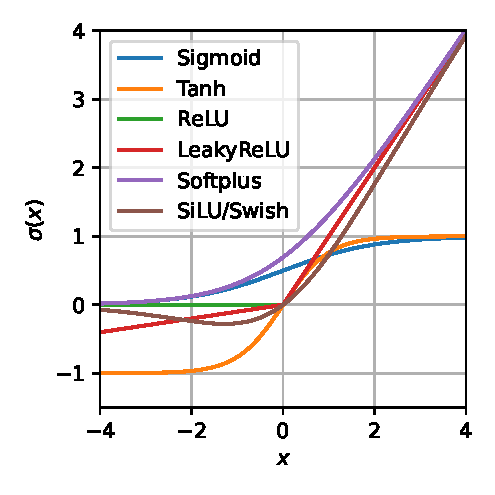
\includegraphics[width=0.4\textwidth]{Figures/transformers/activations.pdf}
    \caption{Common activation functions used in deep learning.}
    \label{fig:activations}
\end{figure}

\section{Training with Gradient Descent}

Training a deep neural network is an optimization problem where the best parameters $\theta^*$ of the network are those that minimize the combined loss $\mathcal{L}$ over the training set $\mathcal{D}$.
\begin{equation}
    \theta^* = \argmin_{\theta} \frac{1}{N} \sum_{i=1}^N \mathcal{L}(\theta, x_i).
\end{equation}
Here the loss function includes some empirical risk calculation and the sample $x \in \mathcal{D}$ is used as shorthand to denote the full sample from the training set, including the target if present.
Due to the size of the parameter space and the non-linearity of the model, the $\theta^*$ can not be found analytically.
The most common method for training deep neural networks is mini-batch stochastic gradient descent (SGD) or one of its many variants~\cite{Perceptron}.
SGD is an iterative optimization algorithm that attempts to minimize a loss function by adjusting the parameters of the model in the direction of the negative gradient of the loss.
The training set is partitioned into batches of size $B$ which are iterated through.
At each iteration, the loss for the batch is calculated, and the parameters are updated using gradient descent with some learning rate $\eta$,
\begin{equation}
    \theta \leftarrow \theta - \eta \nabla_{\theta} \frac{1}{B} \sum_{i=1}^B \mathcal{L}(\theta, x_i).
\end{equation}
Both the $B$ and the $\eta$ are hyperparameters of the training algorithm.
Once the entire training set has been processed, this is considered one epoch.
Training continues until some stopping criterion is met, such as a saturation of the loss.
Typically, models are trained for many epochs and the training set is shuffled between each epoch to prevent correlated updates which may hinder convergence.
Ideally we would have $B=N$, this is called batch gradient descent.
However, this is often infeasible due to memory constraints.
So instead we use a noisy estimate of the gradient, by using a subset of the training set.
True SGD uses a batch size of $B=1$.

The learning rate is a crucial hyperparameter of the training algorithm, however it is common to modify it during training.
Many large networks require a warm-up phase~\cite{SGDRStochasticGradient} where the learning rate is slowly increased from zero to its maximal.
Without this step, large models like transformers are prone to diverging early in training.
The learning rate is also decayed towards the end of training helping the network converge to a local minimum, avoiding oscillation improving the learning of complex patterns~\cite{HowDoesLearning}.
Often these phases are repeated~\cite{CyclicalLearningRates} or performed once~\cite{SuperConvergenceVeryFast}, ending the training after the first cycle.

There exist many extensions to this basic algorithm that attempt to improve robustness and convergence.
One common method is the accumulation of a moving average of the gradients, analogous to momentum in physics~\cite{Momentum}.
This assists in traversing regions of the parameter space where curvature is higher in one direction than another.
Another common method is the use of adaptive learning rates, where the per parameter learning rate is adjusted based on the fluctuations in the gradient~\cite{Adagrad, RMSProp}.
\Cref{alg:adam} shows the update rule for one of the most common variants, the Adam optimizer~\cite{Adam}, which combines both momentum and adaptive learning rates.
It introduces two hyperparameters $\beta_1$ and $\beta_2$ which control the exponential decay rates of the moving averages.

\begin{algorithm}
\caption{The Adam optimizer, where $\mathcal{L}_B(\theta)$ is the loss calculated over a mini-batch, $\eta$, $\beta_1$, $\beta_2$ are hyperparameters, $t$ is the current iteration and $\epsilon$ is a small constant to prevent division by zero.}
\label{alg:adam}
\begin{algorithmic}[1]
\State $\mathbf{m} \gets 0$ \Comment{Initialize first moment vector}
\State $\mathbf{s} \gets 0$ \Comment{Initialize second moment vector}
\For{each mini-batch}
    \State $\mathbf{g} \gets \nabla \mathcal{L}_B(\theta)$ \Comment{Compute gradients}
    \State $\mathbf{m} \gets \beta_1 \mathbf{m} + (1 - \beta_1) \mathbf{g}$ \Comment{Update biased first moment estimate}
    \State $\mathbf{s} \gets \beta_2 \mathbf{s} + (1 - \beta_2) \mathbf{g} \otimes \mathbf{g}$ \Comment{Update biased second moment estimate}
    \State $\hat{\mathbf{m}} \gets \frac{\mathbf{m}}{1 - \beta_1^t}$ \Comment{Correct bias in first moment}
    \State $\hat{\mathbf{s}} \gets \frac{\mathbf{s}}{1 - \beta_2^t}$ \Comment{Correct bias in second moment}
    \State $\theta \gets \theta - \eta \frac{\hat{\mathbf{m}}}{\sqrt{\hat{\mathbf{s}} + \epsilon}}$ \Comment{Update parameters}
\EndFor
\end{algorithmic}
\end{algorithm}

\subsection{Normalization}

Training via gradient descent requires the gradient with respect to every parameter in the model.
This leads to a balancing problem with the vanishing and exploding gradient problems manifesting as the gradients become too small or too large to be useful for training.
This is especially problematic in deep networks, where the gradients must be propagated through many layers, requiring the repeated application of the chain rule.
As the gradients are linked to the scale of the intermediate tensor representations in each layer, it is good practice to ensure that these are roughly the same scale.
It is common to target activations with a mean of zero and a standard deviation of one by including normalization layers.

Another reason for this is that most activation non-linearities are near zero, \Cref{fig:activations}.
Oversaturating these functions ensure that the layer becomes linear, and the network expressivity decreases.

Normalization starts with the input data, which is often normalized in a preprocessing step and typically is performed using the statistics of the training set.
Variables with long tails are typically transformed to have a more Gaussian distribution, such as by taking the logarithm.
Within the network itself, normalization layers $L_{\text{scale}}$ are used to ensure that the activations of each layer have a mean of zero and a standard deviation of one.
Methods such as batch normalization~\cite{BatchNorm} or layer normalization~\cite{LayerNorm} are widely used and both have been shown to be greatly effective, with LayerNorm seen as essential for transformer neural networks~\cite{AttentionIsAllYouNeed}.

Another crucial feature to stabilise the gradients is to manually clip them before applying the update.
This can be done based on some maximal value, but is more commonly done by scaling the gradient such that their combined norm does not exceed some threshold~\cite{WhyGradientClipping}.

\subsection{Residual Connections}

Residual connections are another simple and effective technique for training deep networks.
Here the learnable transformation of the layer is added to the input, rather than replacing it,
\begin{equation}
    \mathbf{a}_{i+1} = \mathbf{a}_i + f(\mathbf{a}_i),
\end{equation}
where $f$ is the transformation of the layer.
A single operation of this form is called a residual block.
Residual connections have been shown to improve the training of very deep networks, as they allow the gradient to flow directly through the network, bypassing the squashing or exploding of the gradient in the intermediate layers.
Residual connections are a key component of almost all moder arcitectures from convolutional neural networks~\cite{ResNet} to transformers~\cite{Attention}.
The residual connection is usually additive, but other operations exist, for example UNets~\cite{UNet} use concatenation.
If the input and output of the layer have different dimensions, the residual path is adjusted by a minimal transformation, in a convolutional network this is typically a $1 \times 1$ convolution.

The addition of two signal paths can lead to a doubling of variance.
This can cause the network to become unstable, especially in the early stages of training.
One method to circumvent this is the inclusion of a normalization layer after the residual block, as was done in the original transformer architecture~\cite{Attention}, and is referred to as post-normalisation.
However, this was shown to be detrimental to very deep networks and recent methods use pre-normalisation~\cite{PreLN} (PreNorm), where the input to the learnable layer is normalized.
With a PreNorm residual block one can prevent an exploding variance by scaling the residual path by a small constant, such as $\frac{1}{\sqrt{2}}$~\cite{StyleGAN2}.
Recent methods allow this constant to be trainable with some set it to zero at the beginning of training such that the block behaves like an identity function~\cite{ReZero, SkipInit, Fixup}.
This was extended to the LayerScale method~\cite{GoingDeeper}, where a full learnable tensor $\mathbf{L}_s$ matching the output shape of the layer is used to scale the residual path.
It too is initialised to zero, and the network is trained to learn the optimal scaling.
A PreNorm residual block with LayerScale follows,
\begin{equation}
    \mathbf{a}_{i+1} = \mathbf{a}_i + \mathbf{L}_\text{scale} \otimes f( L_{\text{norm}}(\mathbf{a}_i) ),
\end{equation}
and such a large models like transformers.

\section{Generalization}

Generalizaion in the context of ML refers to the ability of a model to perform well on new, unseen data.
This is in most cases the primary goal of training such a model.
As neural networks are highly flexible, it is possible that they can ``memorize'' the training set, achieving a very low loss but failing to generalize to new data.
This phenomenon is called overfitting, and it is a common problem in deep learning.

Detecting overfitting can be done through cross-validation, where the model is trained on a subset of the training data and tested on the rest.
The most simple case of this is to split the available data into a training set and a validation set.
Gradient descent is performed on the training set, but the loss is also calculated over the validation set at regular intervals.
The difference in performance between the training and validation set is a good indicator of overfitting.
Often the model chosen for future applications is the one that performs best on the validation set.

Regularization methods like weight decay, dropout, and drop-path are effective in reducing overfitting by penalizing complex models.
Weight decay places a penalty on the size of the parameters in the network, pushing it towards simpler solutions.
Dropout is a technique where a random subset of the activations in the network are set to zero during training, effectively training an ensemble of models.
Another interpretation is that droupout simply injects
Drop path and stochastic depth is an extension of dropout where entire layers are removed from the network during training.
Data augmentation can also help by artificially expanding the training dataset.
Confusingly, increasing the size of the network can also help prevent overfitting.
This is known as the double descent phenomenon~\cite{UnderstandingDoubleDescent}, whereas the effective model capacity grows, more solutions become accessible, and the model becomes a self ensemble.

Domain shift similar to overfitting, but occurs when the distribution of the training data differs from the distribution of the test data.
This is a significant issue in fields HEP, where models are trained on simulated samples, in order to have access to ground truth labels, but must be applied to real data.
Domain adaptation and adversarial training are methods to address this.

Finally, unwanted biases in the training set can lead to skewed predictions.
The distribution of the target variable acts as a prior for the model, and if this distribution is not representative of the population, the model will make biased predictions.
Reweighting or resampling the training set can help mitigate this.


\chapter{Graph Neural Networks}

% The following discussion on graph neural networks is primarily adapted from \textcite{GraphIntro,RelationalInductiveBiases,GraphRepresentationLearning}.

The philosophy behind graph neural networks (GNNs) is that nature is best understood when broken down into compositional elements.
Understanding these elements and the rules that define their relationships is key to understanding the system as a whole.
This reductionist approach is used by much of the scientific community, and indeed is the basis for all of particle physics.
Graphs are an example of explicitly structured data containing entities and pairwise relations between them.
Relational reasoning is the development of rules or functions that describe how the properties of entities modify the relations between them, and how the relations modify the properties of the entities.
GNNs are a class of deep learning models that operate on graph-structured data and employ relational reasoning complete tasks by directly manipulating the rules, entities, and relations of a system.

An example of successful relational reasoning being used in deep learning outside GNNs is in image processing tasks.
An image is typically represented as a tensor of shape $(H, W, C)$, where $H$ is the height, $W$ is the width, and $C$ is the number color channels, using the pixel values as the tensor elements.
Image processing tasks were once the domain of MLPs \citetemp{MLPforMNIST}.
This meant that the image must first be flattened to a tensor of shape $H \times W \times C$, and then passed through a series of fully connected layers, whereby every element of the input tensor is connected to every element of the output tensor.
While this leads to a flexible model, it also destroys the spatial structure of the image and no reusable relationships or rules are discovered.
Instead, we would like to use a model that preserves the structure of the data.

The building block of the convolutional neural network is a learnable convolutional kernel.
The kernel scans over the input tensor, computing the weighted sum of the elements in the kernel window.
This introduces two key relational inductive biases: locality and translation invariance.
Locality refers to the assumption that the relationship between two elements is stronger if they are close together in the input space.
Translation invariance refers to the assumption that the relationship between two elements is the same regardless of their absolute position in the input space.
Locality is enforced by using a kernel width of limited size and translation invariance is enforced by reusing the same kernel across the input space.
Each convolutional kernel defines a learned and reused rule for how elements within the structure of the input tensor are related.

This is an example of geometric deep learning, also called a relational inductive bias, whereby the known structure of the data is embedding into the architecture of the model itself, rather than being learned directly from the data.
This reduces the number of parameters required in the model, allowing for more statistically efficient learning.

\section{Defining a Graph}

A graph $\mathcal{G}$ is a data structure that consists of a set of $N$ attributed nodes $\mathcal{N} = \{\mathbf{x}_i\}_{i=1}^{N}$ interconnected by a set of $N^e$ attributed edges $\mathcal{E} = \{(\mathbf{e}_{k}, r_k, s_k)\}_{k}^{N^e}$.
Here $\mathbf{e}_{k}$ are the edge attributes, $s_k$ is the index of the sender node and $r_k$ is the index of the receiver node.
The graph is directed and self-loops are allowed.
It is also useful in many contexts to define a global attribute $\mathbf{u}$ which describes the entire graph as a whole.
A singular-graph can be represented as a tuple $\mathcal{G} = (\mathcal{N}, \mathcal{E}, \mathbf{u})$.
The structure of the graph is only defined by the interconnections between the nodes, the actual ordering of the nodes in the set is arbitrary.
Therefore, any operation on the graph should not depend on the ordering of the nodes.
Not that the adjacency matrix of the graph is not explicitly defined, but can be inferred from the elements of $\mathcal{E}$.

This representation of a graph is very general and each of the terms $\mathcal{N}$, $\mathcal{E}$, and $\mathbf{u}$ are optionally included.
For example, set data is a special case of a graph where there are no edges connecting the nodes.
Or we could allow multiple sets of edges to exist between nodes $\{\mathcal{E}^1, \mathcal{E}^2, \ldots\}$, defining a multi-graph.
An undirected graph can be represented using a fully symmetrical edge set.

Each of the edge $\mathbf{x}_i$, node $\mathbf{e}_{k}$, and global $\mathbf{u}$ properties of the graph can be encoded as any type of data, even graphs themselves.
However, in most use cases dealt with in deep learning they are real valued tensors.
It is also common for all the nodes to share the same dimensionality, and the same for the edges, imposing an equivalence between the elements of the set.
These are not strict requirements, but it simplifies the design of the model as it allows operations on the individual elements to be parameterized with standard deep learning building blocks, such as linear layers, MLPs, and CNNs.

Representing a graph in code required tuple or dictionary of real valued tensors $(\mathbf{X}, \mathbf{E}, \mathbf{U})$.
Here, $\mathbf{X} \in \mathbb{R}^{N \times d_x}$, $\mathbf{E} \in \mathbb{R}^{N \times N \times d_e}$, and $\mathbf{U} \in \mathbb{R}^{1 \times d_u}$, where $d_x$, $d_e$, and $d_u$ are the dimensionality of the node, edge, and global features respectively.
The edge matrix is typically ordered such that $\mathbf{E}_{ij}$ is the edge from node $i$ to node $j$.
To represent the existence or absence of an edge between two nodes, a binary adjacency matrix $\mathbf{A} \in \{0, 1\}^{N \times N}$ can be used where $\sum{\mathbf{A}} = N^e$.
Alternatively, one could use a sparse tensor representation, which is more memory efficient but can complicate the implementation of the model.

Almost all GNNs operate on the graph by facilitating message passing between the nodes.
In this framework the nodes send messages to their neighbours.
These messages are then aggregates and used to update the node's attributes.

\begin{figure}
    \centering
    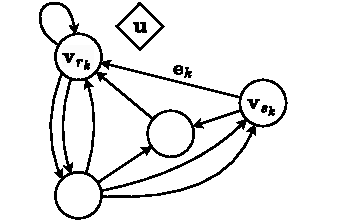
\includegraphics[width=0.5\textwidth]{Figures/transformers/graphs.pdf}
    \caption{A directed multi-graph with node, edges a global attribute $\mathbf{u}$. Highlighted is the edge $\mathbf{e}_{k}$ which connects the sender node $s_k$ to the receiver node $r_k$. Adapted from \textcite{RelationalInductiveBiases}.}
    \label{fig:graph}
\end{figure}

\section{Graph Type Data}

Graph or set representation is fairly ubiquitous in the real world and can be used for anything that can be broken down into discrete elements.
Some examples are shown in \Cref{fig:graph_examples}.
Relevant to this thesis, particle interactions may be expressed as sets, where the stable particles are the nodes.
This is natural representation for particle data, which has no inherent ordering.
Complete interactions and decay chains, like all-hadronic $ttH$ production process shown in \Cref{fig:feynman}, can be represented as a graph.
In this instance, it might be more natural to represent the virtual particles in the Feynman diagram as edges rather than the nodes.
Chemical compounds can be easily represented as graphs, where the atoms and the chemical bonds between them are the nodes and edges respectively.
\Cref{fig:chemical} shows the structure of the antibiotic rifampicin.

Text can be converted into a graph by treating words or subwords as nodes~\citetemp{AttentionIsAllYouNeed}.
Though graphs typically have no natural ordering, it can be imposed by appending the order of the element in the sequence to the attributes of each node.
The edges may also be connected such that they respect the order of the sequence, as in \Cref{fig:text}, where information can only flow forward in the sequence.
This has significant consequences for many generative modelling tasks, essentially providing a natural way to train and perform autoregressive sampling.

Even data which is not inherently graph-like can be broken down into constituent parts and interconnected as desired to form a graph.
Here, the choice of representation is crucial to the rules learned by the model.
As information can only propagate along defined edges in the graph, the existence of an edge implies a direct relationship between the sender and receiver nodes.
An image may be patched into a grid where each patch is treated as a node as shown in \Cref{fig:dog}.
Like the CNN, locality can be imposed by only connecting patches close to each other.
A patched image may not have any edge attributes at all, alternatively, translationally invariant information and could be encoded in the edge attributes, such as the vertical and horizontal distance between patches.

\begin{figure}
    \centering
    \begin{subfigure}[b]{0.45\textwidth}
        \centering
        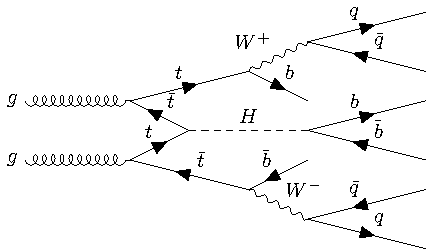
\includegraphics[width=\textwidth]{Feynman/tth.pdf}
        \caption{Particle interactions}
        \label{fig:feynman}
    \end{subfigure}
    \begin{subfigure}[b]{0.45\textwidth}
        \centering
        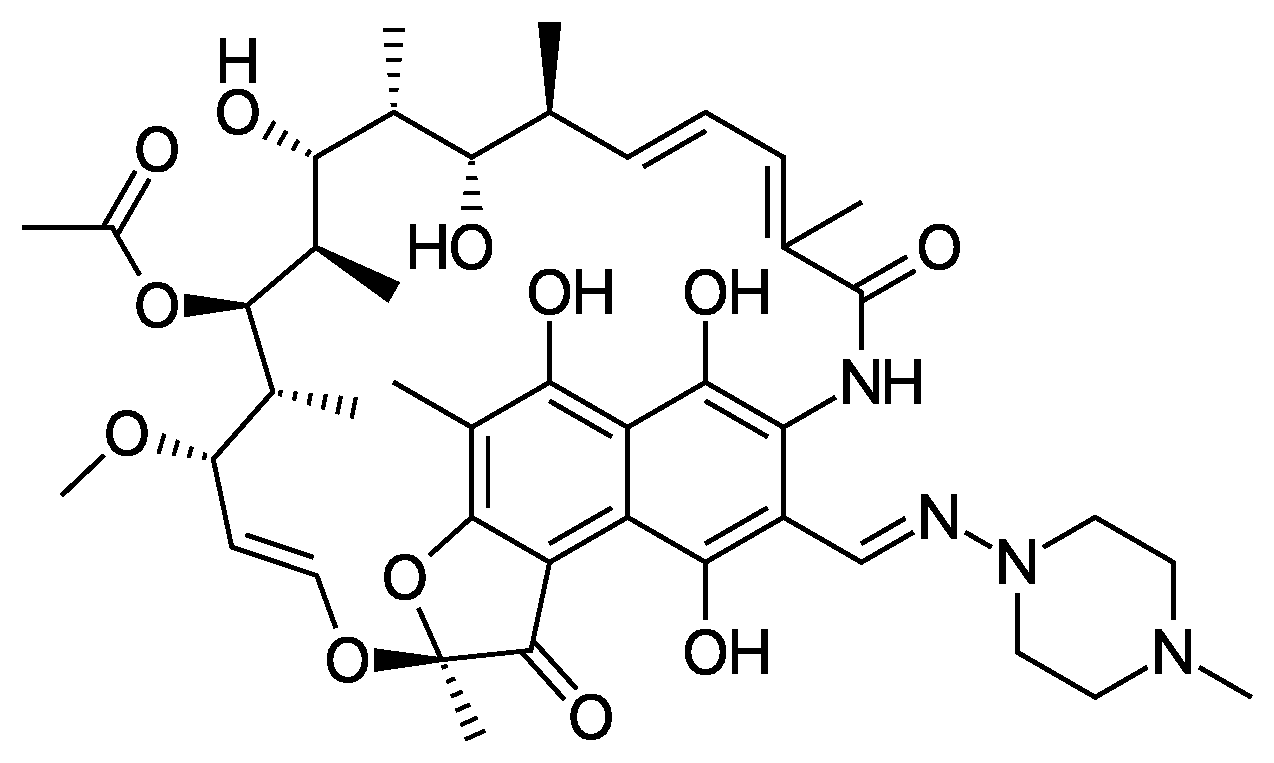
\includegraphics[width=\textwidth]{Figures/transformers/Rifampicin_structure.pdf}
        \caption{Chemical compounds}
        \label{fig:chemical}
    \end{subfigure}
    \begin{subfigure}[b]{0.45\textwidth}
        \centering
        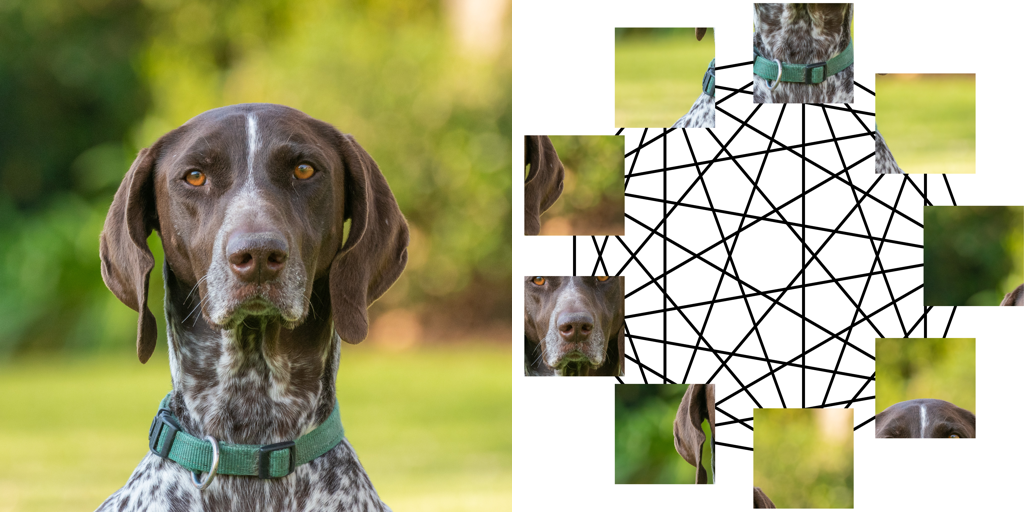
\includegraphics[width=\textwidth]{Figures/transformers/patched_image.png}
        \caption{Images (patched)}
        \label{fig:dog}
    \end{subfigure}
    \begin{subfigure}[b]{0.45\textwidth}
        \centering
        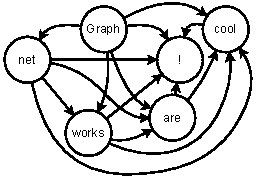
\includegraphics[width=0.8\textwidth]{Figures/transformers/text.pdf}
        \caption{Language (tokenized)}
        \label{fig:text}
    \end{subfigure}
    \caption{Examples of data that can be represented as graphs.}
    \label{fig:graph_examples}
\end{figure}

\subsection{Interconnectivity}

When constructing a graph representation of a data sample, it is crucial to consider its interconnectivity.
The interconnectivity of the graph is closely tied to two key issues in grpah neural networks: the over-squashing problem and the over-smoothing problem.

While locality is often a useful inductive bias, limiting the connections of each node to its local neighbourhood, it can also mean that long term dependencies may get lost.
This is because multiple rounds of message passing are required to propagate information between distant nodes as shown in \Cref{fig:neighbours}.
On each node is the number of message passing steps required to propagate information to the node $\mathbf{x}_i$.
With each round, exponentially more neighbouring nodes need to project information into a fixed-size vectors.
This phenomenon is known as the over-squashing problem, and is exacerbated by bottlenecks in the graph structure as shown in \Cref{fig:bottleneck}, where the information between nodes $\mathbf{x}_i$ and $\mathbf{x}_j$ must pass along a single edge which must also carry information from their respective neighbourhoods.

There are many proposed solutions to the over-squashing problem.
The inclusion of global features in the graph may help model long range dependencies, however the size of the global feature would need to scale with the cardinality of the set.

One solution is to increase the number of edges in the graph, allowing for more direct paths between nodes.
This procedure can be focussed around bottlenecks in the graph, identified by regions of low Forman curvature~\citetemp{Bottlenecks}.
The extreme case of this is a fully connected graph, where edges exist between all pairs of nodes in both directions.
Presenting the data as a fully connected graph allows the model to choose for itself which interactions are important, which it can do if equipped with an attention mechanism~\citetemp{AttentionIsAllYouNeed}.
Attention refers to the process of weighting the incoming messages based before aggregation.
It allows the node to ``pay more attention'' to certain neighbours.
This introduces more expressivity into the model by distinguishing the layers for deciding the content of a message and the layers for deciding its importance.

Using a fully connected graph like this would mean sacrificing the relational inductive bias of locality.
Counterintuitively, this can be beneficial in many cases, for example the most successful models on images use fully connected graphs~\citetemp{VisionTransformers} despite dropping the locality inductive bias of the convolutional kernel.
This is because the locality in images is not always useful, for example if an object in the image is obscured and only partially visible physically separated patches.
In the example of the chemical compound in \Cref{fig:chemical}, the edges are defined by the chemical bonds between the atoms.
However, long range dependencies do exist in chemistry.
The function of one part of a protein may be altered by the presence of a ligand on the other side of the molecule.
Constraining the graph on which the messages are passed to the physical structure of the data may limit the model from learning these relationships.

This highlights a conflict between designing a model strong or minimal inductive biases and whether the computational graph and the input data structure should be tied together at all.
Models such as the perceiver~\citetemp{Perceiver} project input information onto a completly different latent graph and run the message passing on that.
Recent work in vision transformers have shown that the addition of extra, fully learnable nodes to the graph can improve performance~\citetemp{Registers}.

However, there are some downsides to simply increasing the connectivity of the graph.
First, this can be computationally prohibitive when the cardinality of the set is large, as the number of edges grows quadratically.
Many models are looking to find way to minimize the interconnectivity of the graph while preserving model quality~\citetemp{SparseAttention}.
Second, it exacerbates the other problem plaguing GNNs, the over-smoothing problem.
Over-smoothing refers to the phenomenon where the nodes in the graph become homogenous, containing the same information, after many rounds of message passing.
This is because with each round of message passing, the information from the neighbouring nodes is averaged, and the information from the original node is diluted.
This one of the reasons that the depth of most GNNs is notably shallower than other deep learning models.
There are many proposed solutions to this issue, such as residual connections and normalization layers.
Attention is also a viable method to combat over-smoothing.

\begin{figure}
    \centering
    \begin{subfigure}[b]{0.3\textwidth}
        \centering
        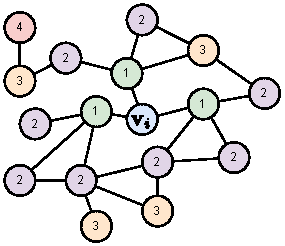
\includegraphics[width=\textwidth]{Figures/transformers/neighbours.pdf}
        \caption{}
        \label{fig:neighbours}
    \end{subfigure}
    \begin{subfigure}[b]{0.3\textwidth}
        \centering
        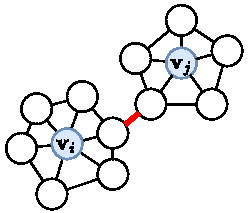
\includegraphics[width=\textwidth]{Figures/transformers/bottleneck.pdf}
        \caption{}
        \label{fig:bottleneck}
    \end{subfigure}
    \caption{\subref{fig:neighbours} The locality of information flow in a graph. \subref{fig:bottleneck} A graph with a bottleneck.}
    \label{fig:over_squashing}
\end{figure}

\subsection{Graph Tasks}

In analysing graph data within real-world contexts, there exists three primary types of predictive tasks: graph-level, node-level, and edge-level predictions.
For graph-level tasks, the aim is to predict an attribute or property that encompasses the entire system as a whole.
An example of this in the context of computer vision would be the classification of the entire image~\citetemp{VisionTransformers}.
Node-level tasks predict the properties associated with each individual node.
They are somewhat analogous to image segmentation.
Finally, there are edge-level tasks which predict  properties or even the existence of edges between the nodes.
An example of this may be predicting the type of virtual particle in a Feynman diagram, \Cref{fig:feynman}.

\section{The Graph Network Block}
\label{sec:gn_block}

The Graph Network Block (GN-Block) is a useful building block for constructing deep learning models that operate on graph-structured data.
It offers a framework that generalizes to many other existing graph-based models, such as graph convolutional networks (GCNs), graph attention networks (GATs), deep sets, and even transformers.
A GN-Block is defined as a series of operations that update the node, edge, and global attributes via facilitating the exchange and aggregation of information according to the structure of the graph.
The GN-Block does not change the cardinality of the features present, only updating their attributes,
\begin{equation}
    \text{GN}(\mathcal{N}, \mathcal{E}, \mathbf{u}) = (\mathcal{N}', \mathcal{E}', \mathbf{u}')
\end{equation}
The GN block is composed of three sub-blocks involving three update functions, $\phi^v$, $\phi^e$, and $\phi^u$, and three aggregation functions, $\rho^{e \to v}$, $\rho^{e \to u}$, and $\rho^{v \to u}$.
Given an input graph $\mathcal{G} = (\mathcal{N}, \mathcal{E}, \mathbf{u})$ the GN-Block proceeds as follows.

\begin{enumerate}
    \item \textbf{Edge Block:} The edges are updated using the current edge attributes, the attributes of the sender and receiver nodes, and the global attribute.
    \begin{equation}
        \mathbf{e}_k' = \phi^e(\mathbf{e}_k, \mathbf{x}_{s_k}, \mathbf{x}_{r_k}, \mathbf{u}).
    \end{equation}
    All edges throughout the graph are updated in this manor which can be executed in parallel.
    The updated edges can be thought of as the message being passed from the sender to the receiver.
    \item \textbf{Node Block:} Incoming edge information is aggregated for each node.
    For node with index $i$, this is represented by the set $E_i$.
    \begin{equation}
        \mathbf{\bar{e}}_i = \rho^{e \to v}(E_i) = \rho^{e \to v}\left(\{(\mathbf{e}_k', r_k, s_k) | r_k = i\}\right)
    \end{equation}
    All nodes are then updated using its current attributes, the aggregated edge information, and the global attribute.
    Updating the nodes using incoming information is called message passing.
    \begin{equation}
        \mathbf{x}_i' = \phi^v(\mathbf{\bar{e}}_i, \mathbf{x}_i, \mathbf{u}).
    \end{equation}
    \item \textbf{Global Block:} All edge information and node information across the graph is aggregated,
    \begin{alignat}{2}
        \mathbf{\bar{v}} &= \rho^{v \to u}(\mathcal{N}') &&= \rho^{v \to u}(\{\mathbf{x}_i\}_{i=1}^{N}) \\
        \mathbf{\bar{e}} &= \rho^{e \to u}(\mathcal{E}') &&= \rho^{e \to u}(\{\mathbf{e}_k'\}_{k=1}^{N^e}),
    \end{alignat}
    and used to update the global attribute,
    \begin{equation}
        \mathbf{u}' = \phi^u( \mathbf{\bar{e}}, \mathbf{\bar{v}}, \mathbf{u}).
    \end{equation}
\end{enumerate}

The GN-Block describes a basic graph to graph transformation which can be composed to form a deeper model.
To make the block learnable, each of the update or aggregation functions may be parameterized by a separate neural network.
The only requirement for any of the aggregation functions is that they are permutation invariant and may accept a variable number of arguments.
This structure also lends itself to the different types of tasks performed on graph type data.
For example, the final GN-Block in the stack may only contain an edge block for an edge-level task.

It is important to investigate exactly what inductive biases are being imposed by the GN-Block.
First, it is clear that the updates to the graph do not depend on the order of the nodes.
Formally, the node and edge updates $(\mathcal{N}, \mathcal{E}) \rightarrow (\mathcal{N}', \mathcal{E}')$ are permutation equivariant to the node set, and the global update $U \rightarrow U'$ is permutation invariant.
The GN-Block applies the same update and aggregation functions to all nodes and edges in the graph.
This reflects the relational inductive bias which seeks to learn general rules that apply to all entities in the system while also adhering to the equivalence of the elements within the set.
Furthermore, as the GN-Block only prescribes the rules for how the features of a graph are updated, it is agnostic to the structure and size of the input graph.
This allows the same model to be applied to input sets with varying cardinality.
This is a crucial feature for many applications, such as particle physics, where the number of particles in an event can vary.
Finally, information flow between elements of the set can follow two paths.
Either, the information propagates along the edges of the graph, enforcing locality, or it is aggregated into the global attribute, then redistributed to the nodes.
This allows for the model to learn both local and long-range interactions.

\section{Different Graph Networks}

A GNN is a general framework for constructing deep learning models that operate on graph-structured data.
Almost all GNNs facilitate message passing and layers within the network can be thought of as some specialization of the GN-Block, depending on the forms of the $\phi$ and $\rho$ functions, and the existence of edge, node, and global features.
The specifics of these functions mean that there are many GNN variants.

A full GN-Block is shown in \Cref{fig:full_gn_block}.
A basic implementation, where all graph attributes are tensors, can be done using MLPs for each of the update functions, and summation for the aggregation functions.
This creates the following update shown in \Cref{alg:gn_block}.

\begin{algorithm}
    \caption{Basic GN-Block using MLPs}
    \label{alg:gn_block}
    \begin{algorithmic}[1]
        \State \textbf{Input:} Graph attributes $\mathcal{G} = (\mathcal{N}, \mathcal{E}, \mathbf{u})$
        \State \textbf{Output:} Updated graph attributes $\mathcal{G}' = (\mathcal{N}', \mathcal{E}', \mathbf{u}')$
        \For{each edge $\mathbf{e}_k$ in $\mathcal{E}$}
            \State $\mathbf{e}_k' \gets \text{MLP}_e([\mathbf{e}_k, \mathbf{x}_{s_k}, \mathbf{x}_{r_k}, \mathbf{u}])$ \Comment{update edge features}
        \EndFor
        \For{each node $\mathbf{x}_i$ in $\mathcal{N}$}
            \State $\mathbf{\bar{e}}_i \gets \sum_{k: r_k = i} \mathbf{e}_k'$ \Comment{aggregate incoming information per node}
            \State $\mathbf{x}_i' \gets \text{MLP}_v([\mathbf{\bar{e}}_i, \mathbf{x}_i, \mathbf{u}])$ \Comment{update node features}
        \EndFor
        \State $\mathbf{\bar{v}} \gets \sum_{i} \mathbf{x}_i'$ \Comment{aggregate features across the graph}
        \State $\mathbf{\bar{e}} \gets \sum_{k} \mathbf{e}_k'$
        \State $\mathbf{u}' \gets \text{MLP}_u([\mathbf{\bar{e}}, \mathbf{\bar{v}}, \mathbf{u}])$ \Comment{update global features}
    \end{algorithmic}
\end{algorithm}

where the square brackets denote tensor concatenation.
This provides a simple model that can be trained end-to-end using gradient descent.
Other GNN layers can be framed similarly.
Even the deep set, which has no pairwise interactions between the nodes can be seen as a reduced form of a GN-Block, as shown in \Cref{fig:deep_set}.
Here the operations are simply,
\begin{align}
    \mathbf{x}_i' &= \text{MLP}_v\left(\left[\mathbf{x}_i, \mathbf{u}\right]\right),\\
    \mathbf{u}' &= \text{MLP}_u\left(\left[\sum_{i} \mathbf{x}_i', \mathbf{u}\right]\right).
\end{align}

GN-Blocks which preserve the existence of graph features, unlike the deep set which has no node features in the output, can be stacked together to form a deep GNN.

\begin{figure}
    \centering
    \begin{subfigure}[b]{0.49\textwidth}
        \centering
        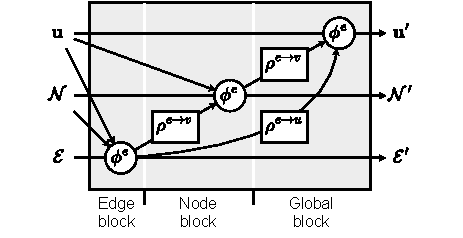
\includegraphics[width=\textwidth]{Figures/transformers/full_gn.pdf}
        \caption{Full GN Block}
        \label{fig:full_gn_block}
    \end{subfigure}
    \begin{subfigure}[b]{0.49\textwidth}
        \centering
        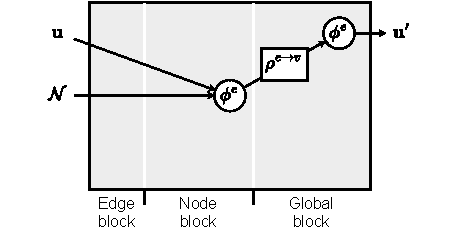
\includegraphics[width=\textwidth]{Figures/transformers/deepset.pdf}
        \caption{Deep Set}
        \label{fig:deep_set}
    \end{subfigure}
    \caption{Examples of different GN-Block implementations \subref{fig:full_gn_block} A full GN-Block has persistent edge and global features. \subref{fig:deep_set} A deep set only applies pooling to the node features to produce a global feature.}
\end{figure}

\section{Transformers are Graph Networks}
\label{sec:transformers}

It is hard to overstate the impact of the transformer model~\citetemp{AttentionIsAllYouNeed} on the field of deep learning.
Originally designed for sequence-to-sequence tasks, transformers grew to dominate all NLP benchmarks.
They marked such a significant improvement that research in other sequence-based models, such as RNNs, almost ceased entirely.
In 2019, Google announced that they were using the transformer based BERT model~\citetemp{BERT} to power their search engine~\citetemp{GoogleBERT}.
They would also switch to using transformers for their translation service~\citetemp{GoogleTranslate}.
Starting in 2018, OpenAI began releasing the GPT~\citetemp{GPT} series of transformer models, arguably triggering a boom around large language models that continues to this day.
In 2020, transformers were adapted to work on image data~\citetemp{VisionTransformers} and have since become the state-of-the-art model for most computer vision tasks, a task that was previously dominated by CNNs, as shown in \Cref{fig:benchmarks}.
Even image generation tasks which one used UNets are now being performed by transformers~\citetemp{DIT, SD3}.
Key to the transformer success is how simple they are to implement and how well the performance seems to scale with the size of the model.
Transformers have become so ubiquitous that they are now considered the default choice for many deep learning tasks, regardless of the data type.

At its core, the vanilla transformer encoder is simply another form of a GNN\@.
There are many variants for the transformer model, but they all share the same basic features.
Contrary to popular belief, these models do not natively run on sequences but on sets, and must be adapted to work on data with an inherent order.
We will focus on two main types of transformers, the transformer encoder and the transformer decoder.
Specifically, the transformer encoder can be seen as a non-local neural network (NLNN)~\citetemp{NLNN} as shown in \Cref{fig:transformer}.
This function operates on a pure set, with no persistent edge or global features.
It involves and message passing step, done using multi-headed attention, followed by a node update step using an MLP.
They also employ residual connections and many forms of normalization to stabilize training and prevent over-smoothing.

The jargon of transformers differs slightly from that of GNNs.
Graphs and sets contain nodes, which are called tokens in many papers on transformers.
The term attention is also used more broadly in transformers, not just referring to the means of weighting an aggregation, it is sometimes used to refer to the entire message passing step.
Furthermore, saying that a node attends to another is equivalent to saying that the node receives a message from the other.
People
The adjacency matrix in a graph is also called the attention mask in a transformer.

\begin{figure}
    \centering
    \begin{subfigure}[b]{0.49\textwidth}
        \centering
        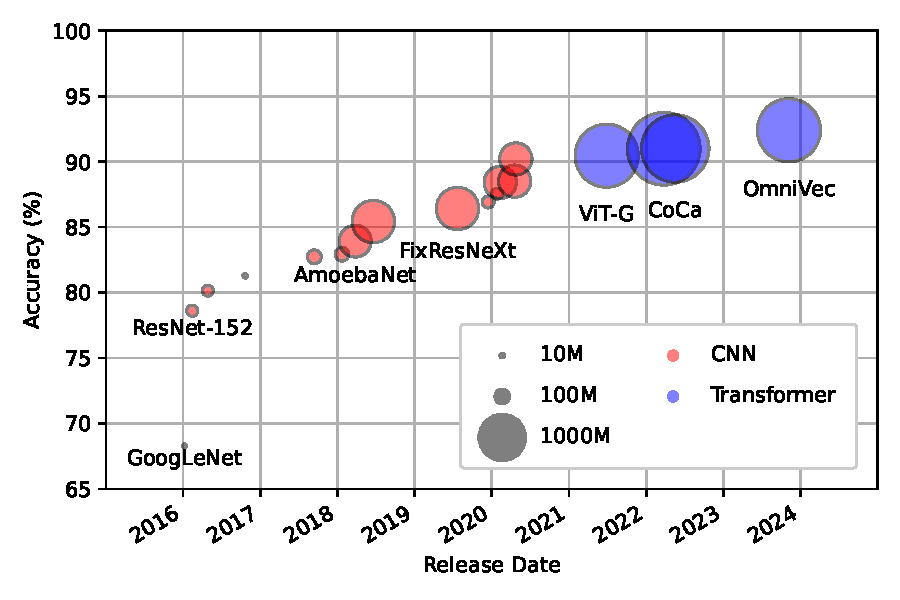
\includegraphics[width=\textwidth]{Figures/transformers/imagenet.pdf}
        \caption{}
        \label{fig:imagenet}
    \end{subfigure}
    \hfill
    \begin{subfigure}[b]{0.49\textwidth}
        \centering
        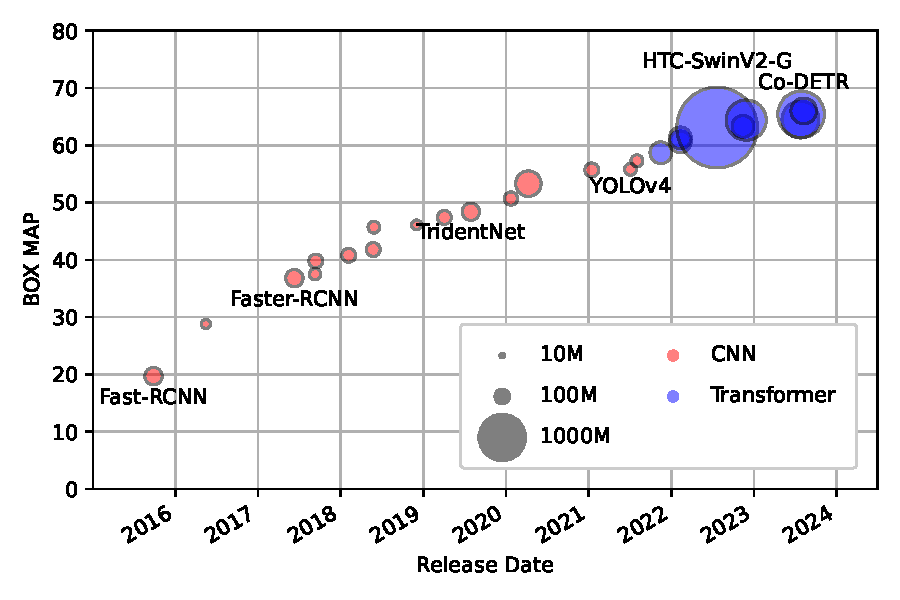
\includegraphics[width=\textwidth]{Figures/transformers/coco.pdf}
        \caption{}
        \label{fig:coco}
    \end{subfigure}
    \caption{Evolution of the state-of-the-art models in two common computer vision benchmarks~\cite{paperswithcode}. The size of the markers corresponds to the number of trainable parameters in the model. \subref{fig:imagenet} Accuracy on the ImageNet classification benchmark, \subref{fig:coco} Bounding box mean average precision (BOX MAP) the COCO object detection benchmark.}
    \label{fig:benchmarks}
\end{figure}

\begin{figure}
    \centering
    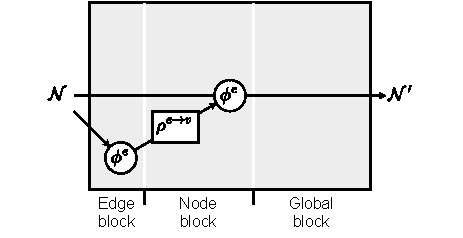
\includegraphics[width=0.49\textwidth]{Figures/transformers/nonlocal.pdf}
    \caption{NLNN / Transformer Encoder}
    \label{fig:transformer}
\end{figure}

\subsection{Attention is Message Passing}
\label{sec:attention}

There are hundreds of ways to parameterize the message passing step in a GNN, and the one used in the transformer is the scaled dot-product attention (SDPA).

In SDPA, the message passed between nodes is a linear projection of the sender node attributes.
This means that each node sends out the same message to all of its neighbours.
This sent information is referred to as the value of the node, where is a learnable weight matrix.
The attention weight is based on a dot product between separate projections of the sender and receiver nodes, called the key and query respectively.
A softmax function is applied to the attention weights to turn the aggregation operation into a weighted mean of the incoming messages.
To prevent the gradients from exploding, the attention logits are scaled by the square root of the dimensionality of the key and value tensors $d_k$.

In the framing of the GN-Block, self-attention has the edge update is factorized into a tuple containing a scalar expressing the message weight $a_k'(\mathbf{x}_{s_k}, \mathbf{x}_{r_k})$ and a vector function for calculating the message content $\mathbf{v}_k'(\mathbf{x}_{s_k})$.
Only $\alpha^e$ depends on the pairwise interaction of both the sender and receiver nodes.
The pooling operation $\rho^{e \to v}$ normalizes over the receiver weights before aggregating the messages.
The block can be written as,
\begin{equation}
    \begin{aligned}
        \mathbf{e}_k' &= \phi^e(\mathbf{e}_k, \mathbf{x}_{s_k}, \mathbf{x}_{r_k}, \mathbf{u}) \\
        &= ( a_k', \mathbf{v}_k' ) \\
        &= \left( \exp \left( \frac{1}{d_k} \mathbf{W}^q \mathbf{x}_{s_k} \cdot \mathbf{W}^k \mathbf{x}_{r_k} \right), \mathbf{W}^v \mathbf{x}_{s_k} \right), \\
        \mathbf{\bar{e}}_i &= \rho^{e \to v}(E_i) \\
       &= \frac{\sum_{k: r_k = i} a_k' \mathbf{v}_k'}{\sum_{k: r_k = i} a_k'}.
    \end{aligned}
\end{equation}
for learnable weight matrices $\mathbf{W}^k \in \mathbb{R}^{d \times d_k}$, $\mathbf{W}^q \times \mathbb{R}^{d \times d_k}$, and $\mathbf{W}^v \in \mathbb{R}^{d \times d_v}$.

This operation can be done efficiently for all nodes in parallel using basic matrix operations.
Furthermore, it allows us to extend to two forms, self-attention and cross-attention, both expressible by the following equation,
\begin{equation}
    \label{eq:attention}
    \text{Attention}(\mathbf{X_r}, \mathbf{X_s}) = \text{softmax}\left(\frac{\mathbf{X_s} \mathbf{W}^q (\mathbf{X_r} \mathbf{W}^k)^T}{d_k} + \mathbf{B}\right) \mathbf{X_s} \mathbf{W}^v.
\end{equation}
In this expression we distinguish between the tensor representing the sender nodes $\mathbf{X_s} \in \mathbb{R}^{N_s \times d}$ and the receiver nodes $\mathbf{X_r} \in \mathbb{R}^{N_r \times d}$.
Self-attention is where the sender and receiver set are the same $\mathbf{X_s} = \mathbf{X_r}$.
This is the standard message passing operation between nodes in a graph.
Cross-attention is where the sender set and receiver set is different $\mathbf{X_s} \neq \mathbf{X_r}$.
This operation is permutation invariant with respect to $\mathbf{X_s}$ and equivariant with respect to $\mathbf{X_r}$.
As shown by \Cref{fig:bipartite}, one can interpret this as the construction of a one-way bipartite graph between two sets, where all nodes in the sender set send messages to all nodes in the receiver set.
The output of the operation would therefore be the updates to the receiver nodes.
Note that the cardinality of the sender and receiver sets do not need to be the same.
Cross-attention is a powerful tool to condition one set on another and is used in many sequence to sequence tasks, from translation to image captioning and text to image generation.
Finally, the bias term $\mathbf{B}$ is a matrix of shape $(N_r, N_s)$ which is broadcasted to the shape of the attention logits.
This can be used to focus or ignore certain pairs of nodes.

\begin{figure}
    \centering
    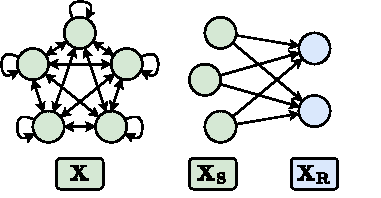
\includegraphics[width=0.5\textwidth]{Figures/transformers/bipartite.pdf}
    \caption{(left) Self-attention is standard message passing between all nodes in a graph. (right) Cross-attention creates a one-way bipartite graph between two sets of nodes.}
    \label{fig:bipartite}
\end{figure}

The final major feature of a transformer's message passing step is multi-headed attention (MHA), shown in \Cref{fig:mha}.
This is where the operation is performed multiple time in parallel with different matrices $\mathbf{W}^q$, $\mathbf{W}^k$, $\mathbf{W}^v$, and $\mathbf{B}$.
The output of each head is concatenated and then mixed using a final linear layer.
\begin{equation}
    \begin{aligned}
    & \text{Head}_1 = \text{Attention}(\mathbf{X_r}, \mathbf{X_s}), \\
    & \ldots, \\
    & \text{Head}_H = \text{Attention}(\mathbf{X_r}, \mathbf{X_s}), \\
    \vphantom{x} \\
    & \text{MHA}(\mathbf{X_r}, \mathbf{X_s}) = \text{Concat}(\text{Head}_1, \ldots, \text{Head}_H) \mathbf{W}^o,
    \end{aligned}
\end{equation}
By performing the operation many times like this, many types of messages are passed between the nodes.
One can also think of this as constructing a multi-graph with different edge types each facilitated by a different head.
Both self and cross attention can be multi-headed where multi-headed self-attention (MHSA) is defined as $\text{MHSA}(\mathbf{X}) = \text{MHA}(\mathbf{X}, \mathbf{X})$.

\begin{figure}
    \centering
    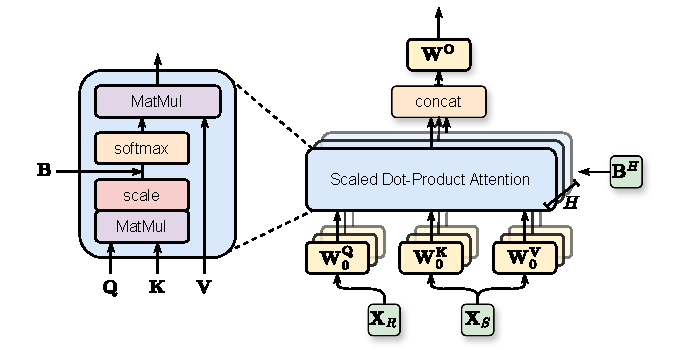
\includegraphics[width=0.5\textwidth]{Figures/transformers/mha.pdf}
    \caption{Multi-headed attention can be thought of as constructing a multi-graph with different edge types.}
    \label{fig:mha}
\end{figure}

While it is not a mathematical requirement, in practice the MHA operation is typically non-resizing, the output matches the input tensor $\mathbf{X_r}$ in shape $(N_r, d_x)$.
The SPDA mechanism requires the query and key dimensions to be the same, but in most implementations the value dimension is also matches.
This means that a single MHA function is parametrized by four weight matrices each with shape $(d_x, d_x)$.
Thus the only hyperparameter for the block is the number of heads $H$, which is required to divide into the node dimension.
One can change value and query projections from linear to affine transformations by including bias terms to increase the expressivity of the model, but the bias of the key operation is completly redundant~\citetemp{RoleOfBiases}.

One of the other keys to the transformer's success is the ease of implementation.
Many of the GNN variants require custom libraries and are difficult to implement from scratch.
However MHA can be implemented in PyTorch using standard linear algebra operations as shown in \Cref{code:attention}.
All heads are computed in parallel using smart reshaping of the tensors.
This is quite significant, as it eases the process of designing, building, testing, and exporting models.
\begin{figure}
    \centering
    \scriptsize
    \begin{minted}{python}
    class Attention(nn.Module):
        def __init__(self, dim: int, num_heads: int):
            super().__init__()
            self.NH = num_heads
            self.HD = dim // num_heads
            self.scale = self.HD**-0.5
            self.wk = nn.Linear(dim, dim)
            self.wq = nn.Linear(dim, dim)
            self.wv = nn.Linear(dim, dim)
            self.wo = nn.Linear(dim, dim)

        def forward(self, xr: T.Tensor, xs: T.Tensor, bias: T.Tensor | int = 0) -> T.Tensor:
            q, k, v = self.wq(xs), self.wk(xr), self.wv(xs)              # project
            shape = (xr.shape[0], -1, self.NH, self.HD)                  # split heads
            q, k, v = (t.view(shape).transpose(1, 2) for t in (q, k, v))
            attn = (q @ k.transpose(-2, -1))                             # attention weight
            attn = (attn * self.scale + bias).softmax(dim=-1)
            x = attn @ v                                                 # aggregate
            x = x.transpose(1, 2).reshape(B, N, D)                       # mix heads
            return self.wo(x)
    \end{minted}
    \caption{A simple implementation of a multi-headed attention block in PyTorch.}
    \label{code:attention}
\end{figure}

\subsubsection{Efficiency of Scaled Dot-Product Attention}

SDPA is arguably the most efficient form of expressive message passing suitable for fully connected graphs.
To show this it is worth starting from the simplest GNN variant, the graph convolutional network (GCN)~\citetemp{GCN}, and seeing why it fails.
The GCN is a form of NLNN where each node sends the exact same message to all other nodes; a simple linear transformation of its own attributes.
The features are then replaced by a sum over incoming information.
A GCN layer can be written as (without normalization factors),
\begin{equation}
    \begin{aligned}
    \mathbf{e}_k' &= \mathbf{W} \mathbf{x}_{s_k}, \\
    \mathbf{x}_i' &= \sum_{k:r_k=i} \mathbf{e}_k',
    \end{aligned}
\end{equation}
for a single learnable weight matrix $\mathbf{W}$.
Lets consider the shapes of the tensors in this operation.
If we represent the set of nodes as a real valued tensor, it will have shape $(N, D)$, where $D$ is the dimensionality of the attributes.
The operation $\mathbf{W}: (N, D) \rightarrow (N, D)$ is efficient, but why this fails to form good representations is clear if we consider the case where the graph is fully connected and the number of edges is $N^2$.
Since all nodes have access to all others, including themselves, however after a single update step every node in the set will contain the same information, taking the over-smoothing problem to the extreme.

To prevent this from happening, each message must be unique for each possible pairing of nodes.
So the issue becomes; what is the most efficient way to parameterize a message such that the output of the message passing must be a tensor of shape $(N, N, D)$?
Here, the first dimension is over the sender nodes and the second dimension is the receiver nodes.
The pooling operation would act over the first dimension to produce a tensor of shape $(N, D)$.
\begin{align}
    \text{??}: (N, D) & \rightarrow (N, N, D) \\
    \text{pool}: (N, N, D) & \rightarrow (N, D)
\end{align}
The GN-Block offers a way to perform this by making the message depend on a concatenation of the sender and receiver attributes.
This concatenation must be done for all possible pairings before passing this tensor through an MLP.
The operations and dimensions of the tensors of such a block are,
\begin{align}
    \text{concatenate}: (N, D) & \rightarrow (N, N, 2D) \\
    \mathbf{MLP}: (N, N, 2D) & \rightarrow (N, N, D) \\
    \text{sum}: (N, N, D) & \rightarrow (N, D)
\end{align}
Even if we were to use a single linear layer rather than an MLP, having both the input and output tensor be $O(N^2)$ is computationally expensive.

One way to mitigate this is to factorize the message into two learnable components, the content and the weight.
Only one of these needs to be unique for each pairing and since the weight is a scalar and the content is a vector, it is much more efficient to allow the content to be degenerate.
This is exactly the approach of GATs~\citetemp{GAT}, which perform the update,
\begin{align}
    \mathbf{W_1}&: (N, D)  \rightarrow (N, D) \\
    \text{concatenate}&: (N, D)  \rightarrow (N, N, 2D) \\
    \mathbf{W_2}&: (N, N, 2D)  \rightarrow (N, N) \\
    \text{matrix multiply}&: (N, N), (N, D)  \rightarrow (N, D)
\end{align}
However, there is still the issue that this input and output of the learnable layers are $O(N^2)$.

The $(N, N)$ matrix of attention weights needs to be learnable from the original $(N, D)$ node attributes and must be allowed to be unique for each pairing.
Therefore, there must be a distinction between the sender and receiver nodes, this makes the required map $a: (N, D), (N, D) \rightarrow (N, N)$.
There are few operations that can achieve this, and none so efficient as a dot product.
Using linear projections for the initial embeddings means that the K, Q, V tensors can be computed in parallel.
\begin{align}
    \mathbf{W}: (N, D) & \rightarrow (N, 3D) \\
    \text{split}: (N, 3D) & \rightarrow (N, D), (N, D), (N, D) \\
    \text{scale-dot-softmax}: (N, D), (N, D) & \rightarrow (N, N) \\
    \text{matrix multiply}: (N, N), (N, D) & \rightarrow (N, D)
\end{align}
While the other parts of the update do require $O(N^2)$ operations, crucially the input and output of the learnable layers dependent is only $O(N)$.

The argument made here is that one will struggle to find a more simple and efficient way to parameterize the message passing step in a GNN that does not lead to over-smoothing when fully connected.
The philosophy of the transformer is similar to the philosophy of composing MLPs from linear layers, in that the composition of simple, highly parameterized functions, is what provides expressivity.
By and large the most complex component of the operation is the softmax function, but there exist algorithms to calculate this online without having to express the full attention matrix~\citetemp{FlashAttention}.
Contrary to popular claims, self-attention with these mechanisms is non $O(N^2)$ in memory complexity~\citetemp{MemoryComplexity}.
Some more recent models large models have even done away with the softmax, citing better performance beyond a certain model scale~\citetemp{Reformer, LinearAttetnion}.

\section{Transformer Variants}

There are many types of transformer variants, too much to cover in this thesis.
However, common similarities can be drawn between them.
Furthermore, many of the terminology used to describe the layers is ambiguous and overlaps.
A single transformer block has two main types of sub-blocks, the message passing layer performed with MHA, and node update layers performed using MLPs, often confusingly called FFNs.
These sub-blocks are combined, and repeated in various forms to create the larger transformer block.
The MHA layers are configured to be either self-attention or cross-attention as needed, and they are stacked with the FFN layers usually in series~\citetemp{AttentionIsAllYouNeed}, but sometimes in parallel~\citetemp{PALM}.
Another distinguishing feature is the use of residual connections and normalization layers to stabilize training.
But even these can be configured in many ways.
With such a large zoo of transformer variants, with empirical performance being the only guide, it often takes time for best practices to emerge.

The MLP in most transformer layers only has a single hidden layer, which expands the dimensionality of the node attributes by a multiplicative factor $M$.
The original implementation used $M=4$ and a ReLU activation function,
\begin{equation}
    \text{FFN}_\text{ReLU}(\mathbf{x}_i) = \max\left(0, \mathbf{W}_2 \text{ReLU}(\mathbf{W}_1 \mathbf{x}_i + \mathbf{b}_1) + \mathbf{b}_2\right),
\end{equation}
though these were quickly switched to either GELU of SiLU activations~\citetemp{GELU, SiLUTransformers}.
Modern transformers also use Gated Linear Units (GLU)~\citetemp{GLU}, a network layer involving the element-wise multiplication of two linear projections, one of which is passed through an activation function.
Using a Swish/SiLU activation function seems to be the most popular choice~\citetemp{SwiGLU}, the node update using a SwiGLU layer is written as,
\begin{equation}
    \text{FFN}_\text{SwiGLU}(\mathbf{x}_i) = \mathbf{W}_3(\text{Swish}(\mathbf{W}_1 \mathbf{x}_i + \mathbf{b}_1) \otimes (\mathbf{W}_2 \mathbf{x}_i + \mathbf{b}_2)) + \mathbf{b}_3.
\end{equation}
Many transformers also use the mixture-of-experts approach, where there exist many FFN layers, each with different parameters, and a gating mechanism to direct certain nodes to certain experts~\citetemp{MoE}.
It is interesting that while the attention mechinism is often hailed as the key to the transformer's sucess, the vast majority of the transformer parameters are in these node update layers.

To stabilize the training of deep models, the transformer encoder uses residual connections and normalization layers.
The residual connection is used to circumvent each sub-block, and in the original implementation used LayerNorm~\citetemp{LayerNorm} after the residual connection.
This was discovered to be over squashing the signal and most modern transformers now use PreNorm configuration where the normalization is done before each sub-block~\citetemp{PreNorm}.
Many models also use RMSNorm as a faster alternative~\citetemp{RMSNorm}.
Furthermore, extra normalization within the sub-blocks is common.
It is also common to initialize the weights of the final layers in each sub-block to zero, or include extra layers initialised close to zero, such that upon initialization the model behaves like an identity function.
This greatly helps to stabilize deeper models.

The transformer encoder (TE) is a standard GNN where the message passing step is performed using multi-headed attention.
It acts on a single set of nodes, and the output of the block is the updated node attributes.
A single TE-Block as shown in \Cref{fig:transformer} is a GN-Block with no edge or global features and the message passing step is done using MHSA.
The block update on the full tensor $\mathbf{X}$, using the PreNorm configuration is,
\begin{equation}
\begin{aligned}
    \mathbf{X} & \leftarrow \mathbf{X} + \text{MSHA}(L_\text{norm}(\mathbf{X})), \\
    \mathbf{X} & \leftarrow \mathbf{X} + \text{FFN}(L_\text{norm}(\mathbf{X})).
\end{aligned}
\end{equation}
A full TE is composed of many TE-Blocks stacked in series forming a permutation equivariant set to set transformation.
For many tasks, the TE is the main feature extractor.

If one wanted to condition the update of one set on another, they could include a multi-headed cross attention operation in the block.
This is the original implementation of the transformer decoder (TD)~\citetemp{AttentionIsAllYouNeed}.
The update is written as,
\begin{equation}
\begin{aligned}
    \mathbf{X}_r & \leftarrow \mathbf{X}_r + \text{MHSA}(L_\text{norm}(\mathbf{X}_r)), \\
    \mathbf{X}_r & \leftarrow \mathbf{X}_r + \text{MHA}(L_\text{norm}(\mathbf{X}_r), \mathbf{X}_s), \\
    \mathbf{X}_r & \leftarrow \mathbf{X}_r + \text{FFN}(L_\text{norm}(\mathbf{X_r})).
\end{aligned}
\end{equation}
The transformer encoder and decoder are often combined to form a set to set transformation that first extracts features from the input set, and the conditions the output set on these features.
This set-to-set transformation is the basis of many generative of sequence-to-sequence models.

\subsection{Edge Attributes, Biases, and Sequences}

When one views the transformer as a simple GNN, the inclusion of edge information become natural.
For message passing on a single graph, when not represented sparsely, the edge information is stored in an $\mathbf{E} \in \mathbb{R}^{N \times N \times d_e}$ tensor.
In the self attention operation in \cref{eq:attention}, the attention matrix defined by,
\begin{equation}
    \mathbf{A} = \text{softmax}\left( \frac{\mathbf{Q} \mathbf{K}^T}{d_k} + \mathbf{B} \right),
\end{equation}
which has the shape $(N, N)$.
When extending this operation to multi-headed attention it gains an extra dimension $(N, N, H)$ matching the required shape of the edge tensor, in fact it is the only valid candidate within the entire operation.
The query and key tensors $\mathbf{Q}$ and $\mathbf{K}$ stem from projections of the input, but $\mathbf{B}$ must have shape which is at least broadcastable to $(N, N, H)$.
Thus edge information can be included in a transformer through the bias term in the attention operation.
This is used in various cases.

The most common use of the bias tensor is to set it manually to negative infinity for certain pairs of nodes and for all heads.
This forces the attention weight to be zero, after the softmax operation, killing the weight of the message entirely.
This enables the transformer to run on graphs which are not fully connected.
It is also one of the main mechanisms for adapting the transformer to work on sequences, where the nodes are presented in a specific order.
By making the bias matrix a lower triangular matrix with above diagonal entries set to negative infinity, each node can only receive messages from those preceding it.
This is also called a causal mask, and is used extensively generative models as it lends itself to autoregressive sampling.
One of the main reasons why the transformer is so successful compared to other sequence models such as an RNN is that a causal attention mask allows it to parallelize training for each element in the sequence with a single forward pass.
During generation of course the model must be run sequentially, but this is a small price to pay for the increase in training speed.
Many sequence generating models are called decoder only, however in the presented framework, these models are transformer encoders with a causal mask.

While can be shown that a causal mask is enough enable the transformer able to run on sequence data, it is often paired with positional encoding.
Absolute positional encoding (APE) adds to the node attributes knowledge of their position within the sequence.
A unique tensor $\mathbf{p}_i \in \mathbb{R}^{d_x}$ is constructed for each posible observed position $i$ and is added to the node attributes before the first transformer block, $\mathbf{x}_i \leftarrow \mathbf{x}_i + \mathbf{p}_i$.
The original transformer used fixed sinusoidal functions of different frequencies to encode the position, but more recent models allow $\mathbf{p}_i$ to be fully learnable~\citetemp{GPT}.
PE is also used for images in, often called spatial encoding, where the 2D coordinates of a patch are individually encoded and added to the patch representation.

APE is not effective for allowing the model to capture the relative position of the elements in the sequence, and for this we turn to relative positional encoding (RPE)~\citetemp{RPE}.
RPE is used to bias the attention matrix and can thus be thought of as a form of edge information.
As with all transformer features, there are many approaches to RPE.
One such method to parameterise $B$ as a Toeplitz matrix, where the elements of the matrix are learnable~\citetemp{RPE}.
ALiBi~\citetemp{ALiBi} fixes the elements of this matrix to be simply $B_{ij} = m\times(i - j)$, for a fixed per-head scalar $m$.
Rotary Positional Encoding is a form of RPE where the query and key tensors are rotated by a fixed amount before the attention operation~\citetemp{RotaryPE}.

Other than positional encoding, transformers can incorporate edge information that are not dependant on order.
The Particle Transformer (PartT)~\citetemp{PartT} uses a transformer encoder to embed a set of particles, defined by their kinematics.
For each pair of particles, specific edge features are constructed using Lund Plane variables~\citetemp{LundPlane}.
The model uses an MLP to embed these edge features into a tensor of shape $(N, N, H)$, which becomes the attention bias in each of the TE-Blocks.

\subsection{Global Attributes and Conditioning Graph Updates}

Global attributes are common features in graphs, and are often used to condition the main node update or are used as outputs of the model.
Global attributes in a GNN are often updated via pooling information across all nodes in the graph $ \mathbf{u} = \rho^{v \to u}(\mathbf{X})$.
This is done in the transformer by simply summing the node attributes.
However, keeping with the theme, the cross-attention mechanism provides a pooling operation that is more expressive, even when the cardinality of the receiving set is one.
This is often called class attention~\citetemp{GoingDeeper}, and in many vision transformer models in order to classify the image as a whole.
The class attention operation can be described as,
\begin{equation}
    \mathbf{U} \leftarrow \mathbf{U} + \text{MHA}(\mathbf{U}, \mathbf{X}),
\end{equation}
where the initial embeddings of the global attributes are learnable.
This process can also be repeated to perform multiple rounds of pooling.

An alternative method relies on the fact that since most transformers act on fully connected graphs, information is not localized.
Therefore, one can simply append a new global toke (often called a class token) to the set which is updated in the same way as the other nodes~\citetemp{VisionTransformers}.
Then to classify the set, class token is read off from the final layer of node attributes.
Recent work on vision transformers have shown that using multiple global tokens in this way, called registers~\citetemp{Registers}, can improve the performance of the model.
Registers can even be ignored from the model outputs, which means that they provide the model with a temporary memory that can be used to store global information.
This is because it was observed that the models had a tendency to overwrite patches with low local information content.

One can use global attributes or extra conditional information to augment the message passing step.
If the global attributes are a set, then cross attention can be used to pass information back and forth between the nodes and global attributes~\citetemp{PCDroid}.
If the global attribute is a single tensor, then cross attention will not suffice.
This is due to the softmax operation in the attention mechanism.
If there is only one sender node, then the attention weight will always be one.
Instead, the global attribute can be concatenated directly in different parts of the block.
This is commonly seen in diffusion models where TE-Blocks must incoroprate time information, expressed as an encoded vector.
This can be done by concatenating the $mathbf{u}$ vector to all node attributes during the MHA step~citetemp{DiffT} or the MLP step~citetemp{PCJedi}.
However the most effective way has been to combine adaptive normalization and residual gating mechanisms~citetemp{DiT}.
Here the global attribute is passed through three projections of the same dimensionality as the node attributes.
It is then used to scale, shift and gate the update,
\begin{equation}
    \begin{aligned}
    & \mathbf{u}_\text{scale}, \mathbf{u}_\text{shift}, \mathbf{u}_\text{gate} \leftarrow \text{MLP}(\mathbf{u}), \\
    & \mathbf{x} \leftarrow \mathbf{x} + \mathbf{u}_\text{gate} \otimes f \left(L_\text{norm}(\mathbf{x} \otimes \mathbf{u}_\text{scale} + \mathbf{u}_\text{shift})\right).
    \end{aligned}
\end{equation}
where $f$ is either the FF or MHA operation within the block.
One can also initialise the MLP in such a way that the $\mathbf{u}_\text{gate}$ is close to zero at the start of training and that the model is initially an identity function.

\chapter{Flavour Tagging with Graphs and Transformers}

In this chapter we describe the design and implementation new graph networks for flavour tagging.
These models build on GN1, a graph network which uses GATv2 system of message passing~\cite{GATv2}, and can be thought of as an architecture optimization of the already successful flavour tagger used by ATLAS.
The first new model is called GN++ and is based on the full GN-Block architecture described in \Cref{sec:gn_block}, complete with persistent edge information and global attributes.
The second new model is called Spice and is based on the transformer encoder architecture, described in \Cref{sec:transformer}, with the message passing step done using multi-headed SDPA.
Spice would prove to be so performant and efficient that it would form the basis of the new GN2 flavour tagger adopted by the ATLAS collaboration.
One of the observations made over the course of this project is that the rate of progress in machine learning is much faster than in high energy physics.
At the time Spice was being developed and presented to the flavour tagging group, GN1 was still undergoing collaboration.
At the time of writing, GN2 is now being calibrated and significant effort is being use to keep it up to date with the latest developments in machine learning.

\section{Datasets}

The same training and test samples used for the previous flavour taggers, DIPS and GN1, were used.
Further information can be found in Refs. \cite{GN1, AlexThesis}.

Two simulated datasets are used in this work to train and evaluate the models.
The first contains $\ttbar$ events and this covers the low $\pt$ phase space for training the taggers.
The simulation settings for the $\ttbar$ sample are derived from studies to best match jet multiplicity and top quark momentum distributions in data~\cite{ttbar1, ttbar2}.
The second sample contains $Z'$ events included to enhance the training statistics in the high $\pt$ phase space.
The $Z'$ boson is a non-SM particle where both the cross-section of the hard-scatter process and the branching fractions were specifically designed to produce a relatively uniform distribution of jets with $\pt$ up to $5~\TeV$ split equally between $b-$, $c-$, and light-jets.

\subsection{Monte Carlo Samples}

Both datasets are initiated by simulated proton-proton collisions at a center-of-mass energy of $\sqrt{s} = 13$ TeV.

Hard scatter events for the $\ttbar$ sample were generated at next-to-leading order using \textsc{PowhegBox v2} \cite{Powheg1, Powheg2, Powheg3} interfaced with \textsc{Pythia 8.230} \cite{Pythia8} using the \textsc{A14} tune \cite{A14} for parton showering and hadronization.
For the parton distribution functions, the \textsc{NNPDF3.0NNLO} \cite{PDF3.0} set was used for the matrix element calculation while the \textsc{NNPDF2.3LO} \cite{PDF2.3} set was used for the showering.
The cut-off scale parameter for the first-gluon-emission $h_{\text{damp}}$ was set to 1.5 times the top quark mass of $m_t = 172.5~\GeV$.
The $Z'$ sample was generated and showered using \textsc{Pythia 8.212} with the \textsc{A14} tune and the \textsc{NNPDF2.3LO} set of parton distribution functions.

For both datasets, decays of $b-$ and $c-$hadrons are done using the \textsc{EvtGen v1.6.0} package \cite{EvtGen}.
Detector response is performed using the \textsc{Geant4} simulation package \cite{Geant4} with the \textsc{ATLAS} simulation setup \cite{ATLASSim}.
Pileup is modelled by overlaying extra minimum bias events using the \textsc{Pythia 8.160} generator with the \textsc{A3} tune \cite{A3} and the \textsc{NNPDF2.3LO} parton distribution functions.
These signals are combined with the hard scatter events during the digitization step.
Interactions with heavy flavour hadrons and the detector material was not simulated but accounted for in correction factors and systematic uncertainties.
In-time pileup is modelled using an average of 40 interactions per bunch crossing, while out-of-time pileup is modelled using bunch crossings before and after the primary interaction.

\subsection{Selection and Sampling}

The ATLAS flavour tagging uses PFLow jets, which are described in \Cref{sec:jet_reconstruction}.
Jets are required to have $\pt > 20~\GeV$ and $|\eta| < 2.5$.
All jets with $\pt < 60~\GeV$ and $|\eta| < 2.4$ must also pass the tight working point of the JVT algorithm in order to minimise contributions from pileup.
Jets are also discarded is they are found to overlap with a generator-level lepton from a $W$ or $Z$ decay.

The training dataset is a mixture of 70\% $\ttbar$ and 30\% $Z'$ events.
To decorrelate the tagger with respect to the jet $\pt$ and $\eta$, jets are also resampled such that the truth matched $b-$, $c-$, and light-jets have identical distributions in these variables.
After resampling the training set contained a total of 120 million jets split equally between the three jet flavours.
During training, 5\% of this was reserved for hold out validation.
Two statistically independent test samples are each containing 1 million $\ttbar$ and $Z'$ jets respectively.
No resampling is done on the test datasets.

\section{Model Design}

All of the proposed models can be thought of as variations or extensions of GN1.
GN1 introduced the idea of a monolithic graph neural network which would simultaneously perform jet tagging, vertexing, and track identification.
All the proposed extensions follow this same setup but with updates to the message passing step as well as latest trends in architecture design.
From Ref.~\cite{RelationalInductiveBiases} and the design of the GN-Block the proposed updates include, persistent edge information, persistent global information, and node feed-forward layers.
From the modern network design and the current trend of transformers, we include multi-headed SDPA, PreNorm, and residual additive connections.

\section{Input Features}

The inputs to all the models presented in this section are the same.
They include two kinematic jet variables, $\pt$ and $\eta$, and up to 40 tracks associated with the jet.
Each track is represented by a vector containing 21 features, detailed in \Cref{tab:track_features}.
Almost all \ttbar jets contain less than 40 tracks, but a significant fraction of $Z'$ jets contain more, as shown in \Cref{fig:track_multiplicity}.
For these samples only the 40 tracks with the highest IP significance $s(d_0)$ are retained.

\begin{table}[h]
    \centering
    \begin{tabular}{ll}
        \toprule
        \midrule
        \multicolumn{2}{c}{Jet Level Inputs Description} \\
        \midrule
        $\pt$ & Jet transverse momentum \\
        $\eta$ & Signed jet pseudorapidity \\
        \midrule
        \midrule
        \multicolumn{2}{c}{Track Level Inputs} \\
        \midrule
        $q/p$ & Track charge divided by momentum \\
        d$\eta$ & Pseudorapidity of the track, relative to the jet $\eta$ \\
        d$\phi$ & Azimuthal angle of the track, relative to the jet $\phi$ \\
        $d_0$ & Closest distance from the track to the PV in the longitudinal plane \\
        $z_0 \sin \theta$ & Closest distance from the track to the PV in the transverse plane \\
        $\sigma(q/p)$ & Uncertainty on q/p \\
        $\sigma(\theta)$ & Uncertainty on track polar angle $\theta$ \\
        $\sigma(\phi)$ & Uncertainty on track azimuthal angle $\phi$ \\
        $s(d_0)$ & Lifetime signed transverse IP significance \\
        $s(z_0)$ & Lifetime signed longitudinal IP significance \\
        nPixHits & Number of pixel hits \\
        nSCTHits & Number of SCT hits \\
        nIBLHits & Number of IBL hits \\
        nBLHits & Number of B-layer hits \\
        nIBLShared & Number of shared IBL hits \\
        nIBLSplit & Number of split IBL hits \\
        nPixShared & Number of shared pixel hits \\
        nPixSplit & Number of split pixel hits \\
        nSCTShared & Number of shared SCT hits \\
        nPixHoles & Number of pixel holes \\
        nSCTHoles & Number of SCT holes \\
        \bottomrule
    \end{tabular}
    \caption{Input features for the Graph Neural Network Flavour Tagger.}
    \label{tab:track_features}
\end{table}

% - Describe GN1
% - Describe the 3 tier loss
% - Describe the full GNN model
% - Describe the proposed transformer model

\section{Training}

% - Training highlights
% - Loss curves
% - All training parameters

\section{Performance}

% - Output distributions
% - ROC curves
% - Rejection values

\section{Applications}

% - GN2X
% - Current model architecture
% - Current training set
% - Current performance










% \include{Chapters/deep_generative_models}
% \include{Chapters/transformers_flavor_tagging}
\chapter{Probabilistic Generative Models}
\label{ch:generative_models}

Probabilistic generative models (PGMs) are a class of models that either aim to learn the underlying probability distribution of a dataset or at least facilitate means to generate new samples indistinguishable from the data.
It is worth highlighting that there is conflicting terminology and many overlapping definitions in the field of PGMs~\cite{DiscriminativeVsGenerative, MachineLearningDiscriminative}, so we will attempt to directly define the terms used in this thesis.

We assume the existence of some unknown probability density $p_\X(\x): \mathcal{X} \rightarrow \mathbb{R}$ over some random variable $\X \in \mathcal{X}$ which is used to populate the training set $\mathcal{D} = \{\x_i\}_{i=1}^N$.
A PGM with parameters $\theta$ fit using $\mathcal{D}$ allows for the generation of new samples following a close approximation of $p_\X(\x)$, denoted as $p_{\theta}(\x)$.
There exist many types of PGMs; some models such as Normalizing Flows (NFs)~\cite{VariationalInferenceNormalizing} provide an explicit functional form for the density $p_{\theta}(\x)$, while others like Generative Adversarial Networks (GANs)~\cite{GenerativeAdversarialNetworks} implicitly learn the density and only permit sampling from it.

We are often interested in approximating a conditional distribution $p_{X}(\x|\con)$ where $\con$ is some context variable.
Supervised learning can also be described in the framework of conditional generation where, in contrast to the notation in \Cref{sec:supervised_learning}, $\x$ is the target variable, and $\con$ is the input.

This section covers the theory behind the PGMs used elsewhere in this thesis, namely NFs and diffusion models.
These models are nominally used to generate continuous data, which matches much of the data we are interested in generating in the context of HEP.
Generative models on discrete data, such as the autoregressive models used in text generation~\cite{GPT2}, are omitted.
An overview of the models is given in \Cref{fig:generative_models}.

\begin{figure}[ht]
    \centering
    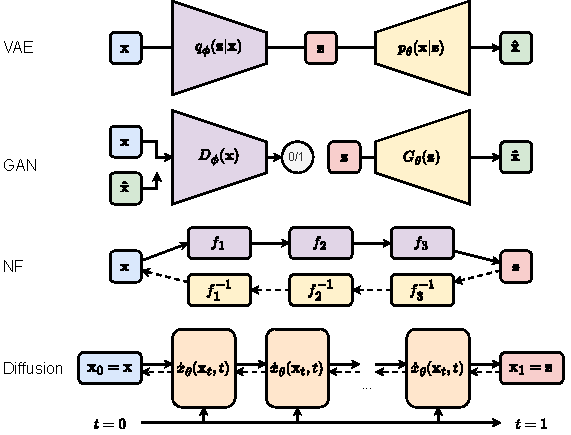
\includegraphics[width=0.8\textwidth]{Figures/generative_models/pgms.pdf}
    \caption{An overview of the generative models covered in this chapter.}
    \label{fig:generative_models}
\end{figure}


\section{Older PGMs}

Over the course of completing this thesis, the field of generative models has seen rapid development.
At the start of this thesis, applications PGMs in HEP mainly involved Variational Autoencoders~\cite{AutoEncodingVariationalBayes} (VAEs) and GANs~\cite{GenerativeAdversarialNetworks}.
While these older models produced impressive results in select domains, the generation quality and fine control we see today in state-of-the-art text-to-image~\cite{SD3, Dalle, Imagen,flux2024github} and text-to-video~\cite{ImagenVideo} models would have been inconceivable a few years ago.
The current landscape of text-to-image~\cite{Imagen, Dalle, SD3}, and even text-to-video~\cite{ImagenVideo} generation would have been inconceivable just a few years ago.
While it is remarkable how quickly the focus on VAEs and GANs has moved on, it is still important to highlight them here for historical context and to better understand the strengths of the models that have replaced them.

\subsection{Variational Autoencoders}

VAEs were introduced in 2013~\cite{AutoEncodingVariationalBayes} and quickly became a popular model for generative tasks, unsupervised learning, and variational inference.
A VAE is an example of a latent variable model.
Here, one introduces a random latent variable $\Z \in \mathcal{Z}$ which one marginalizes over to obtain the distribution of the data,
\begin{equation}
 p_\X(\x) = \int p_{\X,\Z}(\x, \z)\diff\z = \int p_\X(\x|\z)p_\Z(\z)\diff\z.
\end{equation}
The latent space usually covers all real values, $\mathcal{Z} = \mathbb{R}^d$, and the prior $p_\Z(\z)$ is taken to be a simple distribution, such as a diagonal Gaussian $\normal$.
A simple distribution is one that is easy to sample from and the density is easy to calculate.
Practically, we would like to avoid imposing what information is stored in the latent variable.

The standard choice for modelling the likelihood is to use a parametrized Gaussian with constant variance,
\begin{equation}
 p_\X(\x|\z) \approx p_{\theta}(\x|\z) = \mathcal{N}(\x; G_{\theta}(\z), \sigma^2 I),
\end{equation}
where $G_{\theta}$ is a neural network called the decoder.
VAEs introduce an additional parametrized distribution to approximate the posterior which is also taken to be Gaussian with a diagonal covariance matrix,
\begin{equation}
    p_\Z(\z|\x) \approx q_\phi(\z|\x) = \mathcal{N}(\z; \boldsymbol{\mu}_\phi(\x), \boldsymbol{\Sigma}_\phi(\x)).
\end{equation}
Here the estimation of the mean and variance of the approximate posterior is done by a neural network called the encoder and gradients are backpropagated through the stochastic latent variable using the reparametrization trick~\cite{AutoEncodingVariationalBayes}.

One can not train this model by simply maximizing the likelihood of the data, as this is intractable.
However, this form sets up a mapping between the data space to the latent space and back again, and one can train the model by maximizing the evidence lower bound (ELBO).
Practically, this involves minimizing two terms, the reconstruction loss and the KL-divergence between the approximate posterior and the prior,
\begin{equation}
    \mathcal{L}(\theta, \phi) = \mathbb{E}_{\z \sim q_{\phi}(\z|\x)}[||\x - G_{\theta}(\z)||^2] - \beta D_{KL}(q_{\phi}(\z|\x) || p_\Z(\z)),
\end{equation}
where $\beta$ is a hyperparameter that balances the two terms~\cite{BetaVAE}.

Typically, the dimensionality of the latent space is much lower than that of the data space, so the information bottleneck means the model is forced to learn a compressed representation.
VAEs are simple to train but have several limitations.
The bottleneck means that high-frequency detail is dropped, resulting in low-quality samples.
The model is also sensitive to the tuning of $\beta$, often leading to a collapse into one of two regimes.
Either the prior loss dominates, all samples are encoded to the same Gaussian, and all information is lost, or the reconstruction loss dominates.
In the latter case, the learned posterior $q_\phi(\z)$ is non-Gaussian, and extra steps are required to sample from it, such as fitting a kernel density estimator to the empirical distribution of the latent variables~\cite{KDEVAE}.

Conditional information can be injected into the VAE simply by combining the context variable with both the inputs to the encoder and decoder.
The compression of the latent means that it should only store orthogonal information to the context variable, which is useful for disentanglement~\cite{cVAE}.

VAEs were never particularly good at generating high-quality samples, but attempts were still made in HEP to use them for fast simulation of detector responses~\cite{VariationalAutoencodersJet, GraphVariationalAutoencoder, ParticlebasedFastJet}.
They were also used for anomaly detection~\cite{VariationalAutoencodersAnomalous, DeepSetVAE, MassiveIssueAnomaly}.
These applications produced mixed results, and the field has moved on to more powerful models.

\subsection{Generative Adversarial Networks}

Until recently, GANs were the state-of-the-art generative models for producing high-quality samples, most notably demonstrated in generating high-resolution images~\cite{StyleGAN2, StyleGAN3}.
GANs are based on a two-player min-max game between a generator $G_\theta(\z)$ and a discriminator $D_\phi(\x)$, each a neural network with parameters $\theta$ and $\phi$ respectively.
These networks compete in a zero-sum game in which one network's loss is the other's gain.

The generator takes a random latent sample $\z \sim p_\Z(\z)$ and returns a synthetic sample $\hat{\x} = G_\theta(\z) \in \mathcal{X}$.
The discriminator takes samples from both the training set and the synthetic samples and returns a probability that the sample is from the training set, $D_\phi(\x) \in [0, 1]$.
The generator aims to fool the discriminator into thinking the generated samples are real.
Given powerful enough networks, the unique Nash equilibrium of this game is a generator that reproduces the true data distribution and a uniform discriminator output for all samples.

This game has many variations for defining the specifics and loss terms.
The most widely used is the original non-saturating GAN~\cite{GenerativeAdversarialNetworks}.
This loss requires two passes through each network, one to update the discriminator and one to update the generator.
\begin{align}
    \mathcal{L}_{\text{D}}(\phi) &= -\mathbb{E}_{\x \sim \mathcal{D}}[\log D_{\phi}(\x)] - \mathbb{E}_{\z \sim p_\Z(\z)}\log(1 - D_{\phi}(G_{\theta}(\z))], \\
    \mathcal{L}_{\text{G}}(\theta) &= -\mathbb{E}_{\z \sim p_\Z(\z)}[\log D_{\phi}(G_{\theta}(\z))].
\end{align}
Other variants that use different loss derivations exist, such as the Wasserstein GAN~\cite{WGAN1} and the Geometric GAN~\cite{GeometricGAN}.
There is plenty of literature on which variants are best suited for different tasks and which converge to the desired Nash equilibrium~\cite{WhichTrainingMethods}.

The main drawback of GANs is that they are challenging to train.
Often, mode collapse occurs, where the generator exploits a weakness in the discriminator and produces the same samples repeatedly.
Many tricks are required to stabilize training~\cite{WhichTrainingMethods}, such as minibatch discrimination~\cite{ProGAN} and gradient penalties~\cite{WGAN}.
Another drawback to GANs is that it is challenging to produce a conditional generator $G_\theta(\x|\con)$.
Simply concatenating the context variable to both the generator and discriminator inputs leads to mixed results, and the generator is prone to ignoring the context variable~\cite{cGAN}.

In HEP, GANs have mainly been trialled as a method for fast simulation~\cite{MPGAN, GAPT, CaloGAN, EPICGAN}.
However, the main issue is that GANs tend not to cover the full data distribution.
Most of the generation we are looking for in fast simulation is conditional, as detector response depends on the properties of the incoming particle, making GANs not optimal for this task.

\section{Normalizing Flows}
\label{sec:flows}

NFs are a popular tool for both variational inference~\cite{VariationalInferenceNormalizing, NormalizingFlowsProbabilistic}
and density estimation~\cite{NICENonlinearIndependent}.
Like GANs and VAEs, they prescribe a method to train a transformation from a simple latent distribution into one that matches the data.
However, unlike GANs and VAEs, NFs allow for explicit likelihood evaluation, making them much easier to train and well-suited for density estimation.

At the core of NFs is the change of variables formula.
Given two random variables $\X$ and $\Z$ with equal dimensionality related by a diffeomorphism $f: \mathcal{X} \rightarrow \mathcal{Z}$, the probability densities $p_\X(\x)$ and $p_\Z(\z)$ are related by,
\begin{equation}
    \label{eq:change_of_variables}
    p_\X(\x) = p_\Z(f(\x)) \left|\det D f(\x) \right|.
\end{equation}
Here, $f(\x)$ is a differentiable bijective function with a differentiable inverse, otherwise known as a diffeomorphism, and $D f(\x)$ is the Jacobian of the transformation.
The density $p_\X(\x)$ is called a \textit{pushforward} of the density $p_\Z(\z)$ by the function $f$, $p_\X = f_\# p_\Z$.

NFs constructs explicit approximations of data density by defining it as a pushforward of the latent through a parametrized neural network,
\begin{equation}
    p_{\X}(\x) \approx p_{\theta}(\x) = f_{\theta \#} p_\Z(\z) = p_\Z(f_{\theta}(\x)) \left|\det D f_{\theta}(\x) \right|.
\end{equation}
The neural network $f_{\theta}$ must be a diffeomorphism, placing restrictions on the architecture of the network.

Like all neural networks, NFs are built from the composition of several simple layers $f_\theta = f_{\theta_1} \circ f_{\theta_2} \circ \ldots \circ f_{\theta_L}$.
Unlike other neural networks, each \textit{flow layer} has to be a diffeomorphism, as the composition of two diffeomorphisms is itself a diffeomorphism.
The Jacobian of the full transformation is simply the product of the Jacobians of the individual layers,
\begin{equation}
    f_\theta = f_{\theta_1} \circ f_{\theta_2} \circ \ldots \circ f_{\theta_L} \quad \Rightarrow \quad \det D f_\theta(\x) = \prod_{i=1}^L \det D f_{\theta_i}(\x_i).
\end{equation}
This composition property allows us to construct arbitrarily complex transformations, allowing for the approximation any data distribution~\cite{bogachev2005triangular}, using a finite number of layers.

NFs are typically trained via a maximum log-likelihood approach, or more specifically, they use a negative log-likelihood loss function,
\begin{equation}
    \label{eq:nf_loss}
    \begin{aligned}
        \mathcal{L}(\theta)
        \frach &= \mathbb{E}_{\x \sim \mathcal{D}}[-\log p_{\theta}(\x)] \\
        \frach &= \mathbb{E}_{\x \sim \mathcal{D}}\left[-\log p_{\Z}(f_{\theta}(\x)) - \log \left|\det D f_{\theta}(\x) \right|\right] \\
        \frach &= \mathbb{E}_{\x \sim \mathcal{D}}\left[-\log p_{\Z}(f_{\theta}(\x)) - \sum_{i=1}^L \log \left|\det D f_i(\x_i) \right|\right].
    \end{aligned}
\end{equation}
Note that due to the Jacobian's composition property, the log determinant term is a sum of the log determinants of the individual layers, leading to essentially independent contributions per layer in the final loss.

During training, the flow is said to run in \textit{forward-mode}, transforming samples from the data space to the latent space.
Once the model is trained, it can again be used in forward-mode to yield the density at any measured point, or it could be run in \textit{reverse-mode} $f^{-1}$ to generate samples from the data distribution.

Conditional density estimation is a natural extension of NFs.
The only modification is that the context variable is included in the input of each layer in the flow.
This allows the model to learn the conditional distribution $p_{\X}(\x|\con)$ and yields surprisingly good results and highly calibrated uncertainties that match the aleatoric uncertainty in the data almost exactly~\cite{SolvingInverseProblems, InferenceAstrophysicalParameters, ComposingNormalizingFlows, NormalizingFlowsProbabilistic}.
Standard regression, which operates under the assumption of a Gaussian likelihood, is often overly restrictive.
A more effective approach for almost all regression tasks involves framing them as conditional density estimation, where NFs emerge as one of the most suitable tools.

While NFs allow for the exact calculation of the likelihood, they are not without their drawbacks.
The main issue is that NFs are computationally expensive and do not scale well to high-dimensional data.
Even with the specialized flow layers explained in the next section, the complexity of calculating the Jacobian determinant is prohibitive for data with more than a few hundred dimensions.
As NFs describe continuous morphs of data if the latent distribution is connected, so will any learned density.
This causes issues when attempting to model data with disconnected support.
Discrete data needs to be \textit{dequantized} before being fed into the flow to prevent singularities from occurring during training, a notable feature in image modelling where pixel values tend to be quantized to 8-bit integers~\cite{FlowImprovingFlowBased}.

These types of networks have succesfully applied to collider physics, with notable applications including event generation~\cite{EventGen}, template construction~\cite{ANODE, CATHODE, CURTAINs}, unfolding~\cite{PartonsAndBack}, and detector simulation~\cite{CaloFlow, CaloFlow2}.

\subsection{Flow Layers}

Building an NF requires stacking multiple diffeomorphism flow layers together.
They must operate on real-valued tensors $\x \in \mathbb{R}^d$ and optionally include $\con \in \mathbb{R}^c$.
In addition, for practical applications, each layer needs to be efficient to process, both in the forward- and reverse-modes, and the Jacobian determinant should be easy to compute.
The design of these layers is the core research problem in normalizing flows.

At the time of writing, the most popular flow layers are linear flows, coupling flows autoregressive flows, and residual flows.
We describe the ones most relevant to this thesis.

\subsubsection{Linear Flows}

A straightforward, non-resizing linear transform is an example of a flow layer $f(\x) = \W\x + \bias$.
Here, the inverse is simply $f^{-1}(\z) = \W^{-1}(\z - \bias)$.
Only a small amount of reparametrization is required to ensure that the matrix $\W$ is non-singular and thus invertible.
Linear flows are, however, limited in their expressiveness.
Furthermore, the complexity of calculating $\det D f(\x) = |\det \W|$ is $\bigO(d^3)$, making them computationally expensive for high-dimensional data.

One can restrict the form of the matrix to make it easier to use, as shown in \Cref{tab:linear_flows}.
The most popular choices are the LU-Factorisation and, for images, a $1\times1$-convolution~\cite{GlowGenerativeFlow}.

\begin{table}[h!]
    \centering
    \caption{Complexity of using different forms of linear flows.}
    \label{tab:linear_flows}
    \begin{tabular}{ccc}
    \toprule
    \textbf{Type} & \textbf{Inverse} & \textbf{Determinant} \\
    \midrule
    Full & $\bigO(d^3)$ & $\bigO(d^3)$ \\
    Diagonal & $\bigO(d)$ & $\bigO(d)$ \\
    Triangular & $\bigO(d^2)$ & $\bigO(d)$ \\
    Block (c) Diagonal & $\bigO(c^3d)$ & $\bigO(c^3d)$ \\
    LU Factorized & $\bigO(d^2)$ & $\bigO(d)$ \\
    1x1 Convolution & $\bigO(c^3 + c^2d)$ & $\bigO(c^3)$ \\
    \bottomrule
    \end{tabular}
\end{table}

\subsubsection{Coupling Flows}

Coupling flows~\cite{NICENonlinearIndependent} describe a general approach to constructing highly expressive non-linear flows.
In a coupling flow, the input $\x$ is partitioned into two disjoint components $(\x_A, \x_B)$.
$\x_A$ is used to compute the parameters of a bijective transformation called the coupling function $h(\cdot; \phi)$ which is applied to only $\x_B$.
This can be expressed as,
\begin{equation}
    \label{eq:coupling_flow}
    f(\x) = (\x_A, h(\x_B; \phi(\x_A))).
\end{equation}
As shown in \Cref{fig:coupling_flow}, this layer is entirely reversible so long as the coupling function is invertible, whereas the conditioner $\phi$ does not have this restriction.
Additionally, the Jacobian of the transformation is a block matrix given by,
\begin{equation}
    D f(\x) = \begin{pmatrix}
        \mathbb{I} & 0 \\
        \frac{\partial h(\x_B; \phi(\x_A))}{\partial \x_A} & \frac{\partial h(\x_B; \phi(\x_A))}{\partial \x_B}
    \end{pmatrix}.
\end{equation}
When calculating the determinant, the entire bottom left block can be ignored, making it simply the determinant of the invertible transformation $h$.
Thus, $\phi$ can be arbitrarily complex without impacting the convertibility or the computational complexity of calculating the likelihood contributions of the layer.
It is common, therefore, to use a deep neural network for $\phi$ to maximize the expressivity of the layer.
Conditional information can quickly be injected into the flow by incorporating the context variable to the input of the conditioner $\phi(\x_A, \con)$.

\begin{figure}[ht]
    \centering
    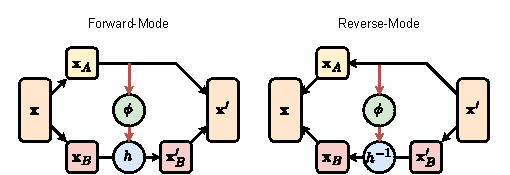
\includegraphics[width=0.8\textwidth]{Figures/generative_models/coupling.pdf}
    \caption{A diagram of a coupling flow.}
    \label{fig:coupling_flow}
\end{figure}

Note that the layer only transforms $\x_B$, leaving $\x_A$ unchanged.
Thus, multiple coupling layers are typically stacked together and interleaved with a fixed random permutation layer or a linear flow to mix the elements of $\x$.
Equivalently, one could also alternate the mask used to partition $\x$ between coupling layers.
Setting $h$ as an elementwise transformation is standard to ensure efficiency.
Early original coupling flows used an affine transformation for $h$~\cite{RealNVP}, which required many layers to fit complex data distributions.
The expressivity of the model can be significantly enhanced using more complex transformations, yet still elementwise bijections, such as rational quadratic splines~\cite{NeuralSplineFlows}.
Splines are especially useful for modelling multimodal data distributions, as single segments within the monotonic splines can become arbitrarily steep, allowing for regions of very low density.
This is demonstrated by \Cref{fig:samples}, which shows the output of a flow with four coupling layers with spline transformations.
The learned densities are shown in \cref{fig:density}.

\begin{figure}[ht]
    \centering
    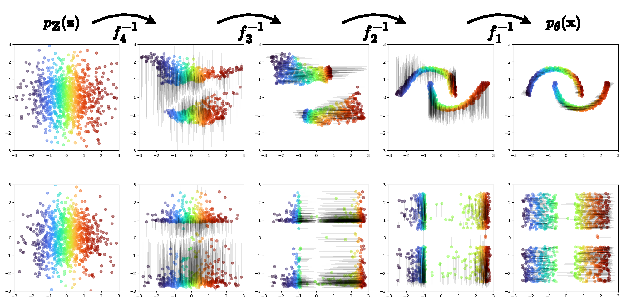
\includegraphics[width=0.95\textwidth]{Figures/generative_models/samples.pdf}
    \caption{The transformation of gaussian samples into a double-moon distribution (top) and a four-box distribution (bottom) using a flow with 4 coupling layers. Each coupling layer can only transform one dimension of the data.}
    \label{fig:samples}
\end{figure}

\begin{figure}[ht]
    \centering
    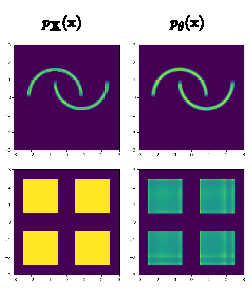
\includegraphics[width=0.4\textwidth]{Figures/generative_models/densities.pdf}
    \caption{The learned (left) and real (right)densities of the double-moon distribution (top) and the four-box distribution (bottom) using a NF.}
    \label{fig:density}
\end{figure}

\subsubsection{Autoregressive Flows}

An autoregressive model is a model decomposes the joint probability distribution into a set of conditional probabilities following a fixed order using the chain rule of probability,
\begin{equation}
    p(\x) = \prod_{i=1}^d p(x_i | x_{<i}).
\end{equation}
In a flow this can be used to define a layer that transforms the data sequentially, where the transformation of each element is conditioned on those previous.
This is called an autoregressive flow~\cite{MaskedAutoregressiveFlow}.
Like a coupling layer, there are two distinct types of transformations in an autoregressive flow, the elementwise transformation $h$ and the conditioning transformation $\phi$.
However, in this case there are $d$ different $\phi$ functions, one for each vector with $d$ elements.
The transformation for the $i$th element is given by,
\begin{equation}
    \label{eq:autoregressive_flow}
    f(\x)_i = h(x_i; \phi_i(x_{<i})).
\end{equation}
The elementwise transformation $h$ are typically the same as those used in coupling layers.
The Jacobian of this transformation is clearly triangular, thus the determinant is simply the product of the diagonal elements,
\begin{equation}
    \det D f(x) = \prod_{i=1}^d \frac{\partial h(x_i; \phi_i(x_{<i}))}{\partial x_i}.
\end{equation}
It is possible to efficiently compute the output of all $phi$ functions in parallel using a single network and a masking scheme~\cite{MADEMaskedAutoencoder}.
This means that the using the flow in forward-mode is highly efficient.
The reverse-mode however must be performed sequentially, as the transformation of each element is conditioned on the previous elements, as shown in \Cref{fig:autoregressive_flow}.
This makes autoregressive flows fast for training but slow for sampling.
Alternatively one could parametrize the layer inversely, choosing efficient sampling but slow training~\cite{ImprovingVariationalInference}.

\begin{figure}[ht]
    \centering
    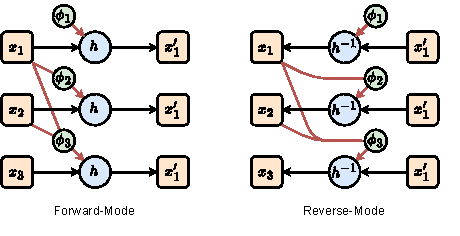
\includegraphics[width=0.8\textwidth]{Figures/generative_models/autoreg.pdf}
    \caption{A diagram of an autoregressive flow. The forward-mode transformation (left) can be computed in parallel, while the reverse-mode transformation (right) must be computed sequentially.}
    \label{fig:autoregressive_flow}
\end{figure}

\subsection{Continuous Normalizing Flows}

Whereas in a standard NF, the transformation is composed of a fixed number of sub-transformations or flow layers, a continuous normalizing flow (CNF)~\cite{NeuralODE} defines a continuous process where each infinitesimal transformation depends on the current state of the data and the time index.
This leads to an ordinary differential equation (ODE) of variable $\x_t \in \mathbb{R}^d$ indexed by $t \in [0, 1]$ defined by a smooth time-varying vector field $u(\x_t, t)$\footnote{We will use $u_t(\x_t)$ and $u(\x_t, t)$ interchangeably.},
\begin{equation}
    \label{eq:cnf}
    \diff \x_t = u_t(\x_t) \diff t.
\end{equation}
Given $\x_0 \sim p_0$, the vector field creates a pushforward $p_t = [\phi_t]_\# p_0$, where $\phi_t$ is the solution of the ODE,
\begin{equation}
    \label{eq:cnf_pushforward}
    \x_t = \phi_t(\x_0) = \x_0 + \int_0^t u_s(\x_s) \diff s.
\end{equation}
The time-dependant density $p_t(\x_t)$ must satisfy the continuity equation,
\begin{equation}
    \label{eq:cnf_continuity}
    \frac{\partial p_t}{\partial t} = -\nabla \cdot (u_t p_t).
\end{equation}
The velocity field $u_t$ is said to be the \textit{probability flow} ODE~\cite{ScoreBasedGenerativeModeling} and $p_t$ is the \textit{probability path} generated by $u_t$.
The induced log-likelihood of the pushforward is given by,
\begin{equation}
    \label{eq:cnf_loglikelihood}
        \log p_t(\x_t)
    = \log p_0(\x_0) - \int_0^t Tr\left(D u_s(\x_s)\right)\diff s
    = \log p_0(\x_0) - \int_0^t (\nabla \cdot u_s)(\x_s) \diff s,
\end{equation}
where $Tr$ is the trace operator.
This relationship was proven in \textcite{NeuralODE}.

To make this model generative, one can set the end-points of the probability path to be the data distribution $p_1 = p_\X$ at $t=1$ and the latent distribution $p_0 = p_\Z$ at $t=0$.
A neural network is then used to learn the velocity field $u_\theta(\x, t): \mathbb{R}^d \times \mathbb{R}_{+} \rightarrow \mathbb{R}^d$ allowing one to interpolate between the two via \Cref{eq:cnf_pushforward}.

Like any flow, the CNF can be trained by maximizing the log-likelihood of the data,
\begin{equation}
    \label{eq:cnf_loss}
    \mathcal{L}(\theta) = \mathbb{E}_{\x \sim \mathcal{D}}\left[\log p_0(\x) - \int_0^1 (\nabla \cdot u_\theta(\x_t, t)) \diff t\right].
\end{equation}
Once the transformation is defined, any numerical ODE solver can transform samples from the data space to the latent space and back again.
This introduces an extra level of complexity when evaluating the model.
A single trained model can have a wide range of behaviour depending on the choice of ODE solver, the number of integration steps, or the use of adaptive step sizes.
With fewer steps, truncation errors during generation can lead to a loss of sample quality, but with more steps, the computational cost of generation increases.

CNFs are highly expressive models but are slow to train.
The loss requires calculating the divergence of the vector field, which is slow to compute in many libraries\footnote{Libraries with advanced automatic differentiation, like JAX\cite{JAX}, can alleviate this issue to a degree}.
Some practical models for low dimensions utilise the Hutchinson trace estimator~\cite{FFJORD},  approximating the trace of the Jacobian with a single Monte Carlo sample.
Even with these optimisations, a single training iteration still requires a full numerical integration of the ODE and subsequent backpropagation through each step, making CNFs impractical for high-dimensional data.


\section{Diffusion Models}

Over the past four years, diffusion models have emerged as the standard for generating high-dimensional data.
Their impact on the landscape of PGMs has been profound.
They have elevated the field from method papers on two-dimensional toy datasets to commercially viable high-resolution text-to-image models which are now ruining the internet.
This significant advancement is primarily due to the exceptionally straightforward training of diffusion models, especially compared to CNFs and GANs.
Their training process is largely stable, with fixed supervised targets.
Furthermore, diffusion models allow for seamless incorporation of contextual generation, enabling fine control over the generated samples.
Finally, the quality of the samples drawn from a diffusion model outperforms all other PGMs.

Diffusion models emerged in 2015~\cite{DeepUnsupervisedLearning}, where the authors were inspired by non-equilibrium statistical physics.
There are three main components to this type of model.
The first is a forward-process that iteratively and systematically destroys structured data by adding noise.
Typically, this is non-learnable and simple to compute.
By the end of the process, any structure is destroyed, and the sample is indistinguishable from pure noise.
A model is trained to learn the reverse-process, which restores the data structure in a similarly iterative scheme.
Generation involves taking a sample of pure noise, typically $\normal$,  and repeatedly applying the reverse-process to modify it into a sample that matches the data distribution.
This defines the final component, the \textit{sampling procedure}, a single trained model can be sampled in many ways, which present trade-offs between speed and quality.
Between 2015 and 2019, the method was largely overlooked, then
In 2020, it was revisited, improved, and applied successfully to images in the form of the Diffusion Probabilistic Models (DDPM)~\cite{DDPM}.
The true research frenzy began in 2021 when diffusion models officially dethroned GANs as the state-of-the-art for conditional image generation~\cite{DiffusionBeatsGANS}.

Many competing, overlapping, and sometimes equivalent frameworks are used to define diffusion models.
They are described through the lens of Markov chains trained via variational inference~\cite{DDPM, DDIM}, score-based models with Langevin Dynamics~\cite{ScoreBasedGenerativeModeling, ElucidatingDesignSpace}, and flow matching with CNFs~\cite{BuildingNormalizingFlows, FlowMatchingGenerative, FlowStraightFast}.
These models share similar training objectives but differ in the mathematical derivations.
Many attempts have been made to unify these models under a framework~\cite{CM2, ElucidatingDesignSpace, UnderstandingDiffusionModels, StochasticInterpolants, FlowStraightFast}.
Since no single framework has emerged as the standard, we will not attempt to unify them here.
However, this chapter uses the term ``diffusion model'' as an umbrella term to describe all of these models, and we chose to focus on two frameworks that are used directly in the projects of this thesis, namely score-based models~\cite{ScoreBasedGenerativeModeling} and flow matching models~\cite{BuildingNormalizingFlows, FlowMatchingGenerative, FlowStraightFast}.

\subsection{Score-Based Generative Models}
\newcommand{\score}{\nabla_{\x_t} \log p(\x_t)}
\newcommand{\cscore}{\nabla_{\x_t} \log p(\x_t|\x_0)}
\newcommand{\unitime}{\mathcal{U}(0, T)}
\newcommand{\timeone}{\mathcal{U}(0, 1)}

Score-based generative modelling~\cite{ScoreMatching, ScoreBasedGenerativeModeling} is a framework that envelops many diffusion models such as DDPM~\cite{DDPM}.
The forward-process involves progressively applying Gaussian perturbations to a data sample in the continuous such that it can be modelled as an SDE,
\begin{equation}
    \label{eq:sde}
    \diff \x_t = \underbrace{f(\x_t, t)}_{\mathclap{\text{drift}}} \diff t + \underbrace{g(t)}_{\mathclap{\text{diffusion}}} \diff \w_t,
\end{equation}
where $\w_t$ is the standard Wiener process (Brownian motion) and $f: \mathbb{R}^d \times \mathbb{R}_{+} \rightarrow \mathbb{R}^d$, $g: \mathbb{R}_{+} \rightarrow \mathbb{R}$ are the drift and diffusion functions respectively, and $t \in [0, T]$ is the time index.
At $t=0$, the sample is uncorrupted\footnote{Note that the time index in diffusion models is typically inverted compared to CNFs}.
Note that if $|g(t)| > 0$ the data signal is progressively corrupted.

While the forward-process is non-learnable, it is not quick to solve without numerical integration.
However, if the drift function is affine with respect to $\x_t$, the transition kernel becomes Gaussian,
\begin{equation}
    \label{eq:gaussian_kernel}
    f(\x_t, t) = f(t)\x_t \quad \Rightarrow \quad p_{0t}(\x_t|\x_0) = \mathcal{N}(\x_t; s(t)\x_0, \sigma(t)^2 \mathbb{I}),
\end{equation}
where $s(t)$ and $\sigma(t)$ are time-dependent scaling factors, referred to as the \textit{signal rate} and \textit{noise rate} respectively, and can be derived for specific forms of $f(t)$ and $g(t)$~\cite{sarkka2019applied}.
Alternatively one can select specific forms for the scaling factors and derive the drift and diffusion functions~\cite{ElucidatingDesignSpace}.
Either way, this choice uniquely defines the \textit{diffusion schedule} for the process, and for generative models one typically constructs it such that,
\begin{equation}
    \label{eq:diffusion_schedule}
    \lim_{t \rightarrow 0} s(t) = 1, \quad \lim_{t \rightarrow 0} \sigma(t) = 0, \quad \lim_{t \rightarrow T} \frac{s(t)}{\sigma(t)} = 0,
\end{equation}
as this ensures that time-dependant marginal of the distribution follows $p_0 = p_\X$ and that $p_\Z \approx p_T = \mathcal{N}(0, \sigma(T) \mathbb{I})$.
Using the transition kernel defined in \Cref{eq:gaussian_kernel}, one is able to sample from the forward-process at any arbitrary time $t$ using the reparametrization trick,
\begin{equation}
    \label{eq:reparametrization}
    \x_t = s(t)\x_0 + \sigma(t) \e \quad \text{where} \quad \e \sim \normal \quad \text{and} \quad \x_0 \sim p_0(\x).
\end{equation}

Remarkably, the SDE in \Cref{eq:sde} has an exact inverse~\cite{ReversetimeDiffusionEquation} which can be used to define the reverse-process,
\begin{equation}
    \label{eq:reverse_sde}
    \diff \x_t = \left[ f(\x_t, t) - g(t)^2 \score \right] \diff t + g(t) \diff \bar\w_t,
\end{equation}
where $\bar\w_t$ is a Wiener process with opposing sign and time flows from $T \rightarrow 0$.
The only unknown term in \Cref{eq:reverse_sde}, $\score$, is referred to as the score function and thus approximating it, called score matching (SM), is the main objective of a score-based generative model.

One naive approach to perform SM is to use direct regression via mean-squared-error which results in the loss function,
\begin{equation}
    \label{eq:naive_loss}
    \mathcal{L}_{SM}(\theta) =
    \mathbb{E}_{t \sim \unitime}
    \mathbb{E}_{\x_t \sim p_t(\x_t)}
    \left|\left|S_\theta(\x_t, t) - \score\right|\right|^2,
\end{equation}
where $S_\theta$ is a neural network with trainable parameters $\theta$.
However, this loss is not practical as it requires the calculation of the very term we are trying to approximate.
One can instead use the denoising score matching (DSM) objective~\cite{ScoreMatching, SlicedScoreMatching} where the conditional score function $\cscore$ is approximated,
\begin{equation}
    \label{eq:denoising_loss}
    \mathcal{L}_{DSM}(\theta) =
    \mathbb{E}_{t \sim \unitime}
    \mathbb{E}_{\x_0 \sim \mathcal{D}}
    \mathbb{E}_{\x_t \sim p_{0t}(\x_t|\x_0)}
    \left|\left|S_\theta(\x_t, t) - \cscore\right|\right|^2.
\end{equation}
This replacement is valid because after taking all expectations, the gradients of the two loss functions are equivalent with respect to the model parameters~\cite{ScoreBasedGenerativeModeling},
\begin{equation}
    \nabla_{\theta} \mathcal{L}_{SM}(\theta) = \nabla_{\theta} \mathcal{L}_{DSM}(\theta).
\end{equation}
This replacement is useful because the conditional score function does have a tractable form due to the transition kernel in \Cref{eq:gaussian_kernel},
\begin{equation}
    \begin{aligned}
        \label{eq:conditional_score}
        \cscore
        &= -\nabla_{\x_t} \log \left( \mathcal{N}(\x_t; s(t)\x_0, \sigma(t)^2 \mathbb{I}) \right) \\
        &= -\nabla_{\x_t} \frac{\left(\x_t - s(t)\x_0\right)^2}{2\sigma(t)^2} \\
        &= \frac{s(t)\x_0 - \x_t}{\sigma(t)^2} \\
        &= \frac{s(t)\x_0 - s(t)\x_0 - \sigma(t)\e}{\sigma(t)^2} \\
        &= - \frac{\e}{\sigma(t)},
    \end{aligned}
\end{equation}
where we have also applied the reparametrization trick from \Cref{eq:reparametrization}.
It is convenient to precondition the network output as,
\begin{equation}
    \label{eq:precondition}
    S_\theta(\x_t, t) = - \frac{\epsilon_\theta(\x_t, t)}{\sigma(t)},
\end{equation}
yielding the final loss function,
\begin{equation}
    \label{eq:noise_loss}
    \mathcal{L}_{DSM}(\theta) =
    \mathbb{E}_{t \sim \unitime}
    \mathbb{E}_{\x_0 \sim \mathcal{D}}
    \mathbb{E}_{\e \sim \normal}
    \frac{\gamma(t)}{\sigma(t)^2}
    \left|\left|\e_\theta(\x_t, t) - \e\right|\right|^2.
\end{equation}
Here, $\gamma(t) > 0$ is introduced as a reweighting factor to balance the loss across the time domain.
Note that by setting $\gamma(t) = \sigma(t)^2$ the loss is uniformly weighted and this often corresponds to good perceptual quality of the generated samples~\cite{VariationalPerspectiveDiffusionBased, VariationalDiffusionModels, ImprovedDenoisingDiffusion}.
Alternatively, one can use specific weighting schemes to allow training on the maximum likelihood objective~\cite{UnderstandingDiffusionModels}.

Once the model is trained, one can define the sampling procedure, which starts from samples drawn from $p_Z=\mathcal{N}(0, \sigma(T) \mathbb{I})$ and numerically integrates the reverse SDE in \Cref{eq:reverse_sde} from $t: T \rightarrow 0$ to obtain samples matching $p_0$.
The integration can be done using the Euler-Maruyama method or stochastic Runge-Kutta methods~\cite{NumericalSolutionStochastic}.
Like CNFs, the generation quality is highly sensitive to the number of integration steps as each step requires another forward pass through the neural network.
The high computational cost of generating a sample with a diffusion model is the main drawback of this approach compared to single-pass methods like NFs and GANs.

As a method to speed up generation, \textcite{ScoreBasedGenerativeModeling} proved the existence of the probability flow ODE whose solutions share the same marginal densities $p_t(\x_t)$ as the SDE.
For the SDE defined in \Cref{eq:sde} it is given by,
\begin{equation}
    \label{eq:probability_flow}
    \diff \x_t = \left[f(\x_t, t) - \frac{1}{2} g(t)^2 \score\right] \diff t.
\end{equation}
Empirically, the probability flow ODE provides a larger tolerance to truncation errors, allowing for fewer integration steps and, thus, faster generation.
In addition, it enables the use of more advanced ODE solvers, provides deterministic encoding, and allows for log-likelihood computation via~\Cref{eq:cnf_loglikelihood}, indicating the strong connection between score-based models and CNFs.
Furthermore, while the probability flow ODE was initially introduced as an alternative method for generation, \textcite{ElucidatingDesignSpace} showed that the entire training objective of a score-based model can be derived purely from an ODE perspective.

\subsection{Conditional Flow Matching}
\label{sec:cfm}

Conditional Flow Matching (CFM)~\cite{BuildingNormalizingFlows, FlowMatchingGenerative, FlowStraightFast} is an alternative framework which arrives at an equivalent training objective to score-based models and can be seen as a method to construct CNFs without the need for numerical integration during training.
The derivation shares many parallels with score-based models, and abundant literature argues their equivalence~\cite{CM2, StochasticInterpolants}.
However, they approach the problem without using SDEs, and like \textcite{ElucidatingDesignSpace}, directly target the probability flow ODE, arguably yielding a more straightforward derivation.

Like CNFs, the goal of CFM is to learn the velocity field $u_t(\x_t)$ that induces the time-dependent density $p_t(\x_t)$ adhering to the boundary conditions $p_1 = p_\X$ and $p_0 = p_\Z$\footnote{Note again that the time index is inverted compared to score-based models.}.
One can express this density as a marginal over a conditional probability path which propagates from a single data sample,
\begin{equation}
    \label{eq:conditional_path}
    p_t(\x_t) = \int p_1(\x_1) p_{t1}(\x_t|\x_1) \diff \x_1.
\end{equation}
The conditional probability path has the endpoints,
\begin{equation}
    \label{eq:conditional_path_endpoints}
    p_{01}(\x_t|\x_1) = p_0(\x_t) \quad \text{and} \quad p_{11}(\x_t|\x_1) = \delta(\x_t - \x_1),
\end{equation}
and is generated by its own conditional vector field $u_t(\x_t | \x_1)$ with the consistency condition,
\begin{equation}
    \label{eq:conditional_consistency}
    \frac{\partial p_{t1}(\x_t | \x_1)}{\partial t} = -\nabla \cdot (u_t(\x_t | \x_1) p_{t1}(\x_t | \x_1)).
\end{equation}

The conditional vector field $u_t(\x_t | \x_1)$ can be used to express the marginal vector field $u_t(\x_t)$ as,
\begin{equation}
    \label{eq:conditional_to_marginal}
    u_t(\x_t) = \int u_t(\x_t | \x_1) \frac{p_{t1}(\x_t | \x_1) p_1(\x_1)}{p_t(\x_t)} \diff \x_1.
\end{equation}
This is proven by,
\begin{equation}
    \begin{aligned}
    \frac{\partial p_t(\x_t)}{\partial t}
    &= \frac{\partial}{\partial t} \int p_{t1}(\x_t | \x_1) p_1(\x_1) \diff \x_1 \\
    &= \int \frac{\partial}{\partial t} p_{t1}(\x_t | \x_1) p_1(\x_1) \diff \x_1 \\
    &= - \int \left(\nabla \cdot (u_t(\x_t | \x_1) p_{t1}(\x_t | \x_1))\right) p_1(\x_1) \diff \x_1 \\
    &= - \nabla \cdot \left(\int u_t(\x_t | \x_1) p_{t1}(\x_t | \x_1) p_1(\x_1) \diff \x_1\right) \\
    &= - \nabla \cdot \left(\int u_t(\x_t | \x_1) \frac{p_{t1}(\x_t | \x_1) p_1(\x_1)}{p_t(\x_t)} p_t(\x_t) \diff \x_1\right) \\
    &= - \nabla \cdot \left(\left(\int u_t(\x_t | \x_1) \frac{p_{t1}(\x_t | \x_1) p_1(\x_1)}{p_t(\x_t)} \diff \x_1\right) p_t(\x_t) \right) \\
    &= - \nabla \cdot \left(u_t(\x_t) p_t(\x_t)\right),
    \end{aligned}
\end{equation}
which is the continuity equation for the marginal density $p_t(\x_t)$.
With this relations we can apply the same trick we did for score-matching, in that the flow matching (FM) loss,
\begin{equation}
    \label{eq:fm_loss}
    \mathcal{L}_{FM}(\theta) =
    \mathbb{E}_{t \sim \timeone}
    \mathbb{E}_{\x_t \sim p_t(\x_t)}
    \left|\left|u_\theta(\x_t) - u_t(\x_t)\right|\right|^2,
\end{equation}
and the CFM loss,
\begin{equation}
    \label{eq:cfm_loss}
    \mathcal{L}_{CFM}(\theta) =
    \mathbb{E}_{t \sim \timeone}
    \mathbb{E}_{\x_1 \sim \mathcal{D}}
    \mathbb{E}_{\x_0 \sim p_0}
    \left|\left|u_\theta(\x_t, t) - u_t(\x_t | \x_1)\right|\right|^2,
\end{equation}
are equivalent with respect to the model parameters $\nabla_{\theta} \mathcal{L}_{FM}(\theta) = \nabla_{\theta} \mathcal{L}_{CFM}(\theta)$~\cite{FlowMatchingGenerative}.

The only remaining feature is to describe the conditional probability path $p_{t1}(\x_t | \x_1)$.
The authors of~\cite{FlowStraightFast} propose a basic Gaussian probability path,
\begin{equation}
    \label{eq:conditional_gaussian}
    p_{t1}(\x_t | \x_1) = \mathcal{N}(\x_t; (1 - t)\x_1, t^2\mathbb{I}),
\end{equation}
which matches the relation in \Cref{eq:gaussian_kernel} by setting $s(t) = 1 - t$ and $\sigma(t) = t$ and allows for the same reparametrization trick for sampling.
This choice is often referred to as the linear interpolation scheme and corresponds to the conditional vector field,
\begin{equation}
    \label{eq:conditional_gaussian_field}
    u_t(\x_t | \x_1) = \frac{\x_t-\x_1}{t}.
\end{equation}
Under the linear interpolation scheme \Cref{eq:cfm_loss} simplifies even further to,
\begin{equation}
    \label{eq:linear_cfm_loss}
    \mathcal{L}_{CFM}(\theta) =
    \mathbb{E}_{t \sim \timeone}
    \mathbb{E}_{\x_1 \sim \mathcal{D}}
    \mathbb{E}_{\x_0 \sim p_0}
    \left|\left|u_\theta(\x_t, t) - (\x_1 - \x_0)\right|\right|^2,
\end{equation}
which is the most common form of the loss used in practice.

Once the network is trained, one can sample from the model by integrating the conditional vector field from noise sample to the data sample as with any CNF.

\subsection{Diffusion Models in Practice}

The training step for most diffusion models is essentially the same.
One samples a time index $t$, a data point $\x \sim p_\X$, and a latent variable $\z \sim p_\Z$.
They are then mixed to get the partially noised sample $\x_t = s(t)\x + \sigma(t)\z$ using predefined scaling factors and passed along with the time index to a neural network.
The network is trained to predict the noise, data point, or velocity field directly.
A trained network defines the ODE or SDE, which can be used to generate samples via numerical integration.
Specifics in this process depend on the choice of framework, the network architecture, and the hyperparameters used.

Over the past four years, some best practices have emerged for training and sampling from diffusion models, such as using slow moving offline networks, targeted time sampling, time encoding, and more advanced ODE solvers.

\subsubsection{Diffusion Frameworks}

Three diffusion frameworks are used in the various projects within this thesis.
The first uses the SM objective by~\textcite{GenerativeModelingEstimating} with trigonometric interpolations~\cite{StochasticInterpolants, ImprovedDenoisingDiffusion}, which we refer to as SM-TI, the second follows the work by~\textcite{ElucidatingDesignSpace} often referred to as EDM diffusion, and the third is the CFM framework by~\textcite{FlowMatchingGenerative, FlowStraightFast, BuildingNormalizingFlows}.
We briefly summarize the main differences in the hyperparameters used in each framework in \Cref{tab:diffusion_frameworks}.

In SM-TI, the diffusion schedule is chosen to be a cosine and sine function such that the total power of $\x_t$, assuming that the training set was standardized, is constant across the schedule.
The network predicts the noise added to the data with the training objective
$\mathbb{E}_{\x, \z, t} \lambda(t) \left|\left| \e_\theta(\x_t, t) - \z\right|\right|^2$.
This is then used to approximate the score function, which is used in either the reverse SDE or the probability flow ODE to generate samples.

In EDM, the diffusion schedule is constructed to simplify the form of the probability flow ODE as much as possible.
Noise is added at a linearly increasing rate to a signal that is kept constant, $\x_t = \x_0 + t\z$.
This results in an ODE with straighter trajectories, which is beneficial for the numerical integration during sampling as it reduces the truncation errors.
The time domain extends to $t_\text{max}$, which also determines the latent distribution's variance and is typically set to be $t_\text{max} = 80$.
The objective is to predict the data itself, with the loss $\mathbb{E}_{\x, \z, t} \lambda(t) \left|\left| f_\theta(\x_t, t) - \x\right|\right|^2$.
The actual network is preconditioned such that
\begin{equation}
    f_\theta = c_\text{skip}(t) \x_t + c_\text{out}(t)F_\theta(c_\text{in}(t)\x_t, c_\text{noise}(t)),
\end{equation}
where $F_\theta$ is the neural network and $(c_\text{skip}, c_\text{in}, c_\text{out}, c_\text{noise})$ are scaling factors.
These factors are manually selected such that the training objective and the network's inputs have unit variance across all values of $t \in [0, t_\text{max}]$.
One can take steps towards the estimated data sample during integration with any ODE.
While this loss was derived without the need for an SDE, the authors of EDM also showed that using a stochastic sampler can improve the quality of the generated samples if enough integration steps are taken.

The CFM framework follows the derivation in \Cref{sec:cfm}, where the diffusion schedule is a basic linear interpolation between the noise and the data and the network target is simply the difference between the two.
CFM has arguably the simplest to implement training loop, which is shown in \Cref{code:cfm}.
This model generated the samples in \Cref{fig:cm_samples}, which includes double-moon and four-box datasets.
One of the main benefits of the CNF framework is that the latent distribution does not have to be Gaussian, and the theory holds for any arbitrary distributions.
The bottom row of \Cref{fig:cm_samples} has the model interpolating from the double-moon distribution to the four-box distribution.

\begin{figure}
    \centering
    \scriptsize
    \begin{minted}{python}
    class CFM(nn.Module):
        def __init__(self, dim, time_dim):
            super().__init__()
            self.mlp = MLP(input_dim=dim, output_dim=dim, context_dim=time_dim)
            self.cos_enc = CosEnc(dim, time_dim)

        def get_loss(self, x0):
            t = T.rand((x0.size(0), 1))                # Sample time
            x1 = T.randn_like(x0)                      # Sample noise
            xt = (1 - t) * x0 + t * x1                 # Linear interpolation
            ut = self.mlp(xt, self.cos_enc(t))         # Predict velocity
            return (ut - (x0 - x1)).square().mean()    # MSE loss
    \end{minted}
    \caption{A simple implementation of the CFM framework in PyTorch. The model is trained to predict the velocity field $u_t(\x_t)$ that interpolates between the noise $\z$ and the data $\x$ at time $t$.}
    \label{code:cfm}
\end{figure}

A natural question arises regarding which of these models performs better.
Research on this topic is ongoing, and the community has yet to reach a consensus.
However, the CFM framework with the linear interpolation diffusion schedule is now used by the majority of commercial diffusion models for text-to-image synthesis.
This includes models such as Stable Diffusion 3~\cite{SD3} and Flux~\cite{flux2024github}, indicating a practical preference for this framework.

{
\renewcommand{\arraystretch}{1.5}
\begin{table}[h!]
    \centering
    \caption{Hyperparameters used in the different diffusion frameworks.}
    \label{tab:diffusion_frameworks}
    \resizebox{\textwidth}{!}{
    \begin{tabular}{cccc}
    \toprule
    & \textbf{SM-TI} & \textbf{EDM} & \textbf{CFM} \\
    \midrule
    time index $t$ & $t \in [0, 1]$ & $t \in [0, t_{max}]$ & $t \in [0, 1]$ \\
    signal rate $s(t)$ & $\cos(\frac{t\pi}{2})$ & $1$ & $1 - t$ \\
    noise rate $\sigma(t)$ & $\sin(\frac{t\pi}{2})$ & $t$ & $t$ \\
    latent distribution & $\normal$ & $\mathcal{N}(0, t_\text{max}^2\mathbb{I})$ & $\normal$ \\
    training target & noise - $\z$ & data - $\x$ & velocity - $(\x - \z)$ \\
    $\frac{\diff \x_t}{\diff t}$ & $- \frac{\pi}{2}\tan(\frac{\pi t}{2})(\x_t - \score)$ & $- t \score$ & $u_t(\x_t)$ \\
    sampling & SDE or ODE & SDE or ODE & ODE \\
    \bottomrule
    \end{tabular}
    }
\end{table}
}

\begin{figure}[ht]
    \centering
    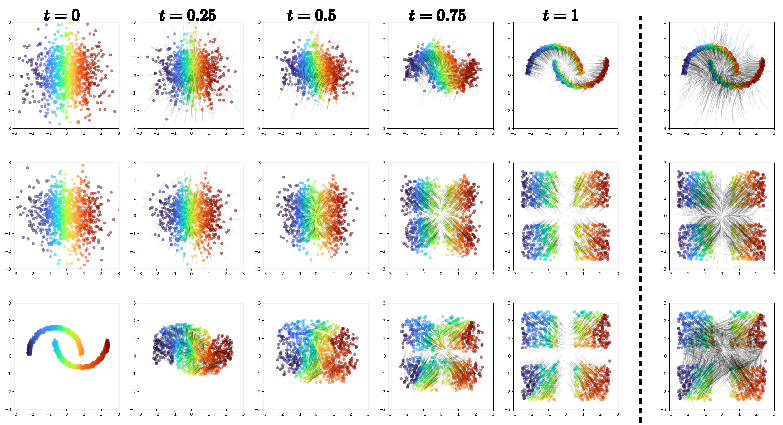
\includegraphics[width=0.99\textwidth]{Figures/generative_models/cm_samples.pdf}
    \caption{The transformation of gaussian samples into a double-moon distribution (top) and a four-box distribution (middle), and the interpolation between the two (bottom). The model was trained using the CNF framework generated with Heun's method~\cite{heun} for 64 steps. Each column shows the samples at a different time index $t$, the black lines trace back to the samples in the previous column. The rightmost column shows the full paths traced by each sample from the base distribution.}
    \label{fig:cm_samples}
\end{figure}


\subsubsection{Conditional Verses Unconditional Paths}

One of the claims of both EDM and CFM is that they lead to straighter trajectories than SM-TI, allowing for faster sampling as fewer steps are needed in the numerical integration.
This is indeed the case, as shown by \Cref{fig:vp_vs_cfm}, where the SM-TI model results in paths with very high curvature, especially at the end of the schedule.
Note that none of the paths are completely straight.
This is because all frameworks were derived using a similar technique to overcome the intractable marginal density (velocity) by using the conditional density (conditional velocity) as a proxy.
This means tension exists between the actual training target and what the model approximates, and this discrepancy is highlighted in \Cref{fig:oned_oned}.
In the latter case, the model was trained to interpolate between samples drawn from the same distribution, meaning that an optimal model would be $u_t(\x_t) = 0$
So, even if the conditional paths are straight, as with EDM and CFM, the marginal paths are not.
This discrepancy results in a few considerations for training.

\begin{figure}[ht]
    \centering
    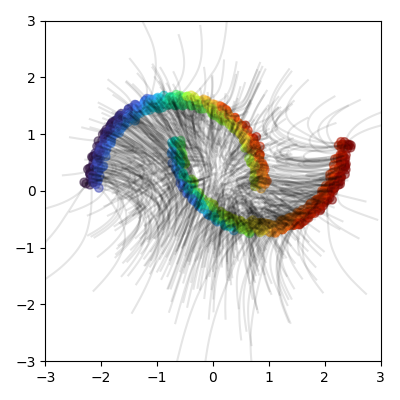
\includegraphics[width=0.45\textwidth]{Figures/generative_models/fm.png}
    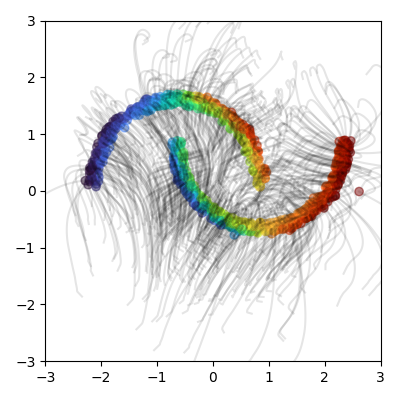
\includegraphics[width=0.45\textwidth]{Figures/generative_models/vp.png}
    \caption{The marginal paths generated interpolating between a Gaussian and a double-moon distribution learned by using the CFM schedule (left) and the SM-TI schedule (right).}
    \label{fig:vp_vs_cfm}
\end{figure}

Using conditional paths as a proxy training target results in unbiased updates with high variance.
While diffusion models are not at risk of collapsing like GANs, gradient updates are highly stochasic, and convergence is slow.
Almost all diffusion models are trained with two copies of the network: an online-network and an offline-network.
The online-network is updated using standard gradient descent, while the offline network is updated using the exponential moving average of the online network.
The offline-network is always used for sampling.
This common trick could be applied to any deep learning task~\cite{Adam}, but it is ubiquitous in diffusion models.

Note that predicting the marginal velocity for CFM is significantly harder in the middle of the schedule than at the endpoints.
This is because the optimal prediction for the marginal velocity at $t=0$ is a vector pointing towards the mean of $p_1$, and the optimal prediction at $t=1$ points towards the mean of $p_0$.
Similarly, at $t=t_0$ in EDM, $f_\theta$ should be the identity function, and at $ t=t_\text{max}$, the ideal denoiser returns the mean of the training set.
Therefore, it is common to use non-uniform sampling for the time index during training to target the time steps where the most information can be gained.
These are typically based on empirical results and are not derived from the theory.
For EDM, $\log(t) \sim \mathcal{N}(-1.2, 1.2)$ was chosen after a hyperparameter search and for CFM it was found that logit-normal sampling,
\begin{equation}
 t \sim \frac{1}{\sqrt{2\pi}}\frac{1}{t(1-t)}\exp\left(-\frac{(\text{logit}(t))^2}{2}\right),
\end{equation}
where $\text{logit}(t) = \log\left(\frac{t}{1-t}\right)$, was the most effective~\cite{SD3}.

\begin{figure}[ht]
    \centering
    \includegraphics[width=0.49\textwidth]{Figures/generative_models/oned2.png}
    \includegraphics[width=0.49\textwidth]{Figures/generative_models/oned.png}
    \includegraphics[width=0.49\textwidth]{Figures/generative_models/oned_target.png}
    \includegraphics[width=0.49\textwidth]{Figures/generative_models/oned2_marginal.png}
    \caption{(left) The conditional paths used to train a CFM, and (right) the marginal paths generated by the model. The top row shows a model interpolating between a two-box distribution and a Gaussian distribution, and the bottom row shows a model interpolating between samples drawn from the same three-box distribution.}
    \label{fig:oned_oned}
\end{figure}

\subsubsection{Straighter Paths and Distillation}

Even with the aforementioned training tricks, the highly variant outputs are still a problem, and much work has been dedicated to learning straighter paths.
Straight paths would be optimal, as they could be solved using a single Euler step.
One approach is to use mini-batch optimal transport couplings between the data and the latent samples before mixing~\cite{ImprovingGeneralizingFlowbased}.
However, this method does not scale well to high-dimensional data, even for mini-batches.
Another approach is to take a trained model and \textit{distil} it by training a second model to learn the same endpoints as the first model but with straighter trajectories.
There are various methods for distillation, such as rectification~\cite{FlowStraightFast}, progressive distillation~\cite{ProgressiveDistillationFast}, and consistency distillation~\cite{ConsistencyModels}.
Each method attempts to reduce the number of inference steps required to generate high-quality samples.

However, there is an argument to be made that the multiple steps make diffusion models so powerful.
Since the process requires removing noise from the data, any additional error terms induced by truncation errors are also removed.
Diffusion models have been described as applying iterative refinements~\cite{ImageSuperResolutionIterative} to the data, and the multiple steps might allow the model to self-correct.

\subsubsection{Time Encoding}

In all models, the network needs to take in time information.
One can do this by simply concatenating the time index to the input, but it is more beneficial to perform positional encoding beforehand.
This is most commonly done using trigonometric functions, such as the positional encoding used in transformers~\cite{Attention}, or random Fourier features~\cite{FourierFeaturesLet}.
However, we have found the most success with a basic cosine-encoding (CosEnc)~\cite{ImplicitQuantileNetworks}.
This layer takes a scalar $t$ and returns an output tensor of length $d$, where each element is the output of a cosine function with exponentially increasing frequency.
The lowest frequency is set such that the layer will not have duplicate outputs.
For parameters $t_\text{min}$, $t_\text{max}$, and $d$ the CosEnc layer is given by,
\begin{equation}
    \label{eq:cosine_encoding}
    \text{CosEnc}(t) =
    \begin{bmatrix}
        \cos\left(e^0 t'\right) \\
        \cos\left(e^1 t'\right) \\
        \vdots \\
        \cos\left(e^{d-1} t'\right)
    \end{bmatrix}, \quad \text{where} \quad t' = \pi \frac{t - t_\text{min}}{t_\text{max} - t_\text{min}}. \\
\end{equation}
This can be seen as a form of continuous binary encoding and can be used in the network layers via adaptive normalization and gating described in~\Cref{sec:global_attributes}.

\subsubsection{Conditional Generation}

Other conditioning information $\con$ can easily be added to the network, such as class labels or other auxiliary information.
This works for all frameworks and requires including the context information with the network inputs, the exact form depending on the model's architecture.
Interestingly enough, one does not even have to train a conditional model to perform conditional generation due to the relation,
\begin{equation}
  \label{eq:conditional_generation}
  \nabla_{\x_t} \cdot \log p(\x_t | \con) = \nabla_{\x_t} \cdot \log p(\x_t) + \nabla_{\x_t} \cdot \log p(\con | \x_t).
\end{equation}
Thus, one only needs a second time-dependent classifier for the conditioning information.
Gradients with respect to this model can be used to modify the update rule for the ODE or the velocity field to perform conditional generation.
This is often referred to as \textit{guidance} in the diffusion literature~\cite{DiffusionBeatsGANS}.

\subsubsection{Sampling}

As previously discussed, various numerical integration techniques can be employed with either the reverse SDE or the probability flow ODE to sample from a diffusion model.
Beyond the conventional numerical integration methods, such as Euler, Heun, and Linear Multi-Step methods~\cite{heun}, a novel domain has emerged, focusing on developing efficient integration methods tailored to specific diffusion schedules.
Notable examples include DDIM~\cite{DDIM}, DPM-Solver~\cite{DPMSolverFastODE}, DPM-Solver++~\cite{DPMSolverFastSolver}, UniPC~\cite{UniPC}, and DPM-Solver-2M~\cite{DPMSolverFastSolver}.
These samplers are adaptable to both stochastic and ordinary differential equations.

Furthermore, the number of integration steps and the step size vary across different methods. In~\cite{ElucidatingDesignSpace}, the integration steps were designed to take larger steps at the beginning of the schedule and smaller steps towards the end, facilitating refinement. This variability complicates the comparison of models, as the same model may yield different results depending on the integration method employed, presenting a significant challenge for benchmarking.


% \include{Chapters/anomaly_detection}
% \include{Chapters/foundation_models_hep}
% \chapter{Conclusion}
\label{ch:conclusion}

This thesis introduced novel methods that utilized deep learning techniques to address various challenges in high-energy physics.
The work has demonstrated the benefits of using state-of-the-art machine learning techniques, such as diffusion models, transformers, and normalizing flows.

\Cref{ch:spice} presented several architecture modifications to the existing flavour tagging model used by the ATLAS collaboration, GN1.
Specifically, the Spice model utilized the transformer and demonstrated significant improvements over GN1 in terms of $b$- and $c$-tagging performance.
It has since been integrated into the ATLAS software framework, forming the new GN2 tagger, which is being actively used in the ATLAS experiment.
The code repository for continuously updating GN2, known as \texttt{Salt}, is available for the broader community to contribute to and use.
Many working groups within ATLAS now use either \texttt{Salt} or GN2 including those that operate outside the flavour tagging domain.
Ongoing work is focused on further improving the model's performance by adopting the latest trends in transformer design in the wider machine-learning community.
Recent additions include reducing the model's memory and time complexity by adding support for highly compressed representations of the input data and efficient attention mechanisms~\cite{FlashAttentionFastMemoryEfficient}.
GN3, the next tagger undergoing development, incorporates particle flow information.
This increasing the cardinality of the input set from an average of 10 to around 100, making the support for efficient training and inference even more critical.

\Cref{ch:neutrino_unfolding} presented a novel method for neutrino unfolding using normalizing flows.
The \vvflows method significantly improved the reconstruction of neutrino kinematics and overall event reconstruction, offering a promising alternative to traditional analytical techniques.
This thesis considered final states with one or two neutrinos.
There is ongoing work to not only extend it to final states with more neutrinos but to also produce a model which can generalize to any number of neutrinos.
This requires swapping out the normalizing flow for a set diffusion model like those presented in \Cref{ch:jet_generation,ch:foundation_models}.

\Cref{ch:jet_generation} presented novel methods for the conditional generation of the particle cloud representation of high-energy physics jets.
These methods were based on the diffusion framework.
\pcdroid performed the showering and hadronization steps typically done by tools such as \pythia and \herwig and saturated many of the metrics used by the community to evaluate generative models on jets.
The model was then extended to full-event generation, showing it could replicate the response and reconstruction steps typically handled by \delphes.
Datasets produced with \delphes tend to be overly idealized and do not model the many intricacies of a full detector simulation.
Future work focuses on moving towards a high-quality simulated dataset using \geant.
The generative models developed in this chapter were applied to a template-based anomaly detection task.
While they proved effective for template generation, the high dimensionality of the point clouds made anomaly detection, which required training a CWoLa model, infeasible at low signal strengths.
This seems to be a limitation of the CWoLa method, so one avenue is to explore other anomaly detection methods that make use of the template generator that does not require training on noisy labels.

\Cref{ch:foundation_models} detailed the development of a foundation model for physics data, introducing self-supervised learning regimes capable of generalizable and meaningful representations of particle physics jets without labelled data.
The proposed methods, MPM and SSFM, demonstrated promising results and are still being developed.
While the field and theory of foundation models remain relatively nascent, significant progress is being made, particularly in optimal fine-tuning strategies such as low-rank adaption~\cite{LoRALowRankAdaptation} and specialized tokens~\cite{ParameterEfficientTuningSpecial}.
Efforts are also directed towards extending the model's applicability to full events with more involved topologies, rather than individual jets.
Work is also being done to integrate the pre-training step into the GN2 pipeline.
This pre-training will be done on actual data, and it is hypothesized that it will mitigate modelling errors in the training set that adversely affect the model's performance.

Moreover, the pre-trained models provide an interesting opportunity for a comprehensive data-driven search for new physics operating on low-level data.
While the tests in \Cref{ch:jet_generation} failed to detect small amounts of signal injected into the data, the results from \Cref{ch:foundation_models} showed that pre-training greatly improved the model's sensitivity to even the lowest levels of signal.
One can envision an anomaly detection pipeline in which the SSFM model is trained on a real data sample, producing both the pre-trained CWoLa classifier and a pre-trained generator for the template generation.

A potential shortcoming of the research presented in this thesis is that, aside from the findings in \Cref{ch:spice}, there is an overreliance on parametrized simulation tools like \delphes to generate training data.
The use of \delphes was necessary because there were very few high-quality datasets at the start of this research.
Several datasets had to be made explicitly for the research presented in this thesis, such as the ones used in \Cref{ch:neutrino_unfolding}.
Many of the other datasets, such as the JetNet and LHCO datasets used in \Cref{ch:jet_generation}, and the JetClass dataset used in \Cref{ch:foundation_models}, are frequently used in the machine-learning/HEP community, but are not based on full detector simulations.
This is more of a critique of the current state of the field.
However, this trend is changing, and efforts are being made to release full-simulation datasets from the CMS and ATLAS experiments publicly.
Future work will undoubtedly benefit from the use of higher-quality data.


\appendix

% \include{Appendices/AppendixA}

\printbibliography[heading=bibintoc]

\end{document}
